\section{Apéndice}
\label{sec:apendice}

    \subsection{Resultados completos del escenario de carga sobre el sistema base}
    \label{sec:resultados_completos_sistema_base_baseline}

        \begin{figure}[H]
            \centering
            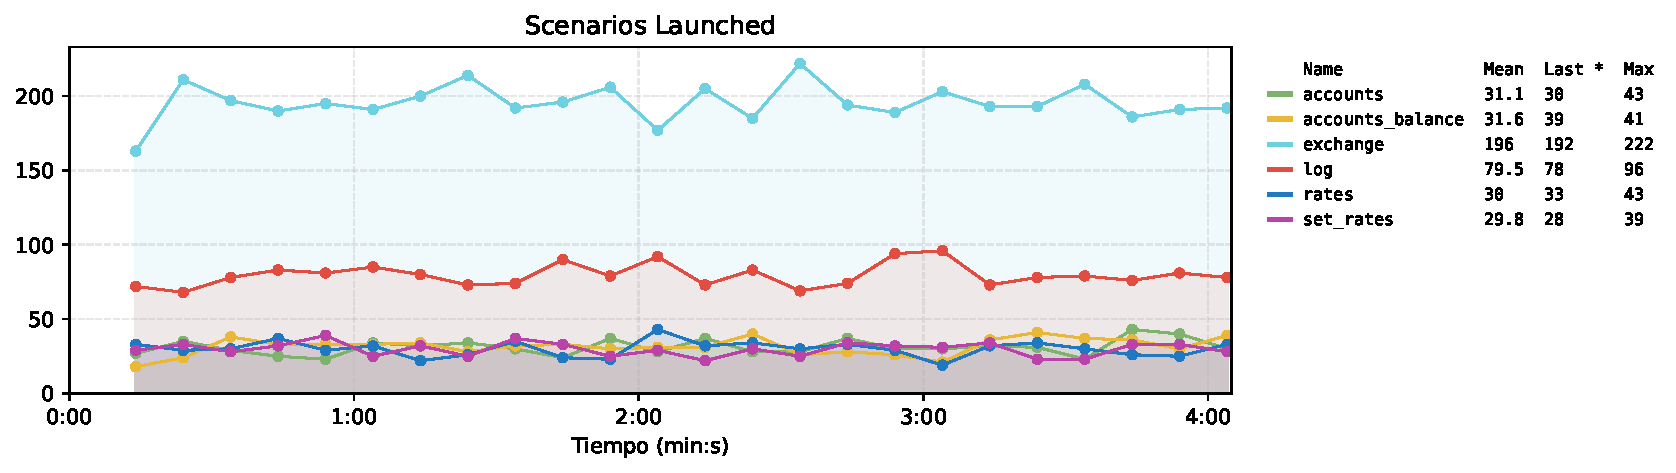
\includegraphics[width=0.8\columnwidth]{figures/sistema_base/baseline/scenarios}
            \caption{ Escenarios del sistema base. }
            \label{fig:resultados_completos_sistema_base_baseline_scenarios}
        \end{figure}

        \begin{figure}[H]
            \centering
            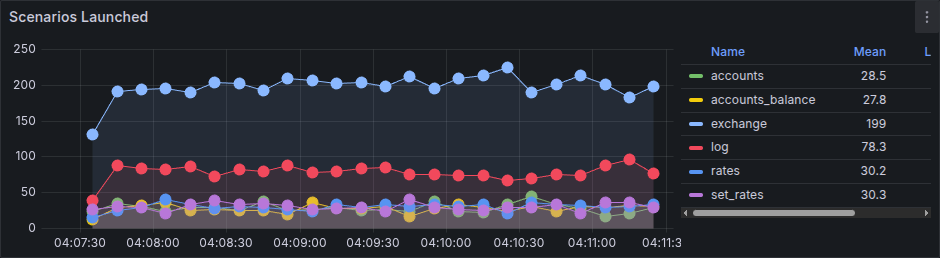
\includegraphics[width=0.8\columnwidth]{figures/sistema_base/baseline/scenarios_captura}
            \caption{ Se adjunta la captura correspondiente a la Figura~\ref{fig:resultados_completos_sistema_base_baseline_scenarios}. }
            \label{fig:resultados_completos_sistema_base_baseline_scenarios_captura}
        \end{figure}

        \begin{figure}[H]
            \centering
            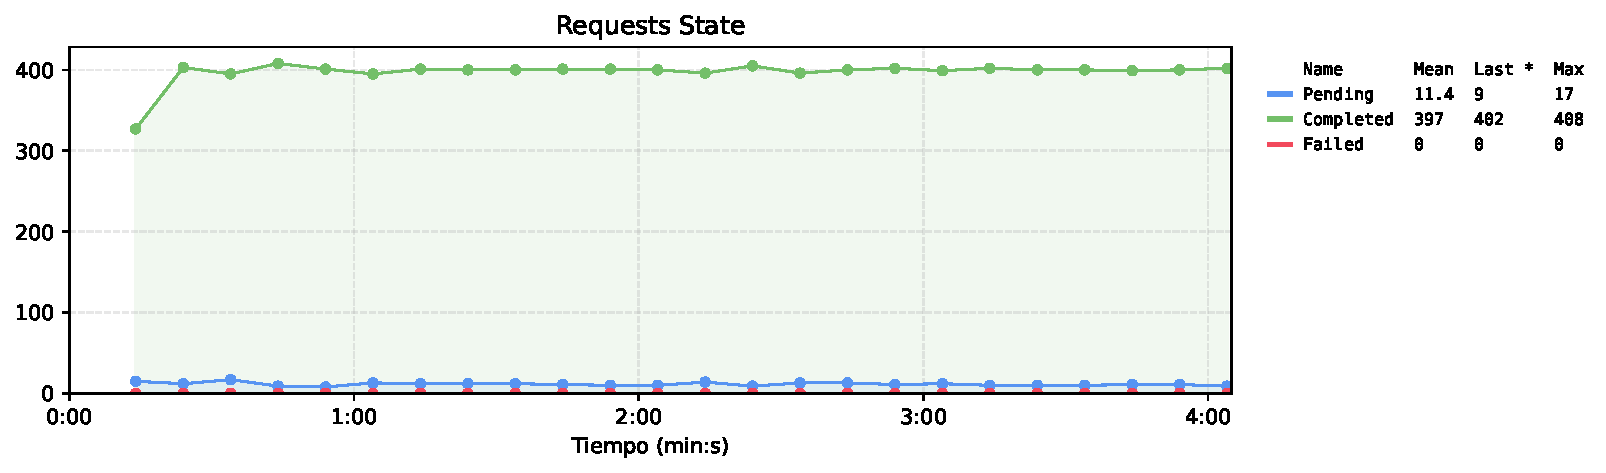
\includegraphics[width=0.8\columnwidth]{figures/sistema_base/baseline/requests_state}
            \caption{ Estado de las requests del sistema base. }
            \label{fig:resultados_completos_sistema_base_baseline_requests_state}
        \end{figure}

        \begin{figure}[H]
            \centering
            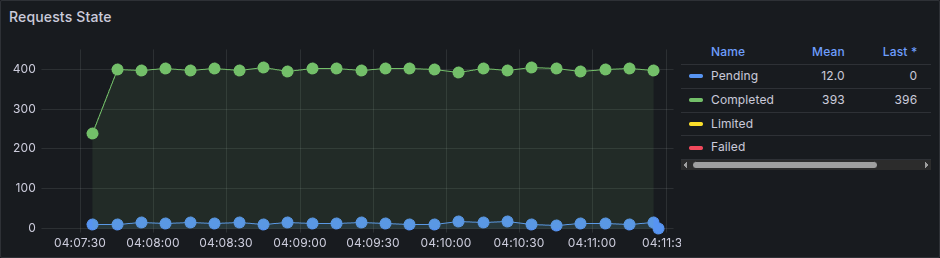
\includegraphics[width=0.8\columnwidth]{figures/sistema_base/baseline/requests_state_captura}
            \caption{ Se adjunta la captura correspondiente a la Figura~\ref{fig:resultados_completos_sistema_base_baseline_requests_state}. }
            \label{fig:resultados_completos_sistema_base_baseline_requests_state_captura}
        \end{figure}

        \begin{figure}[H]
            \centering
            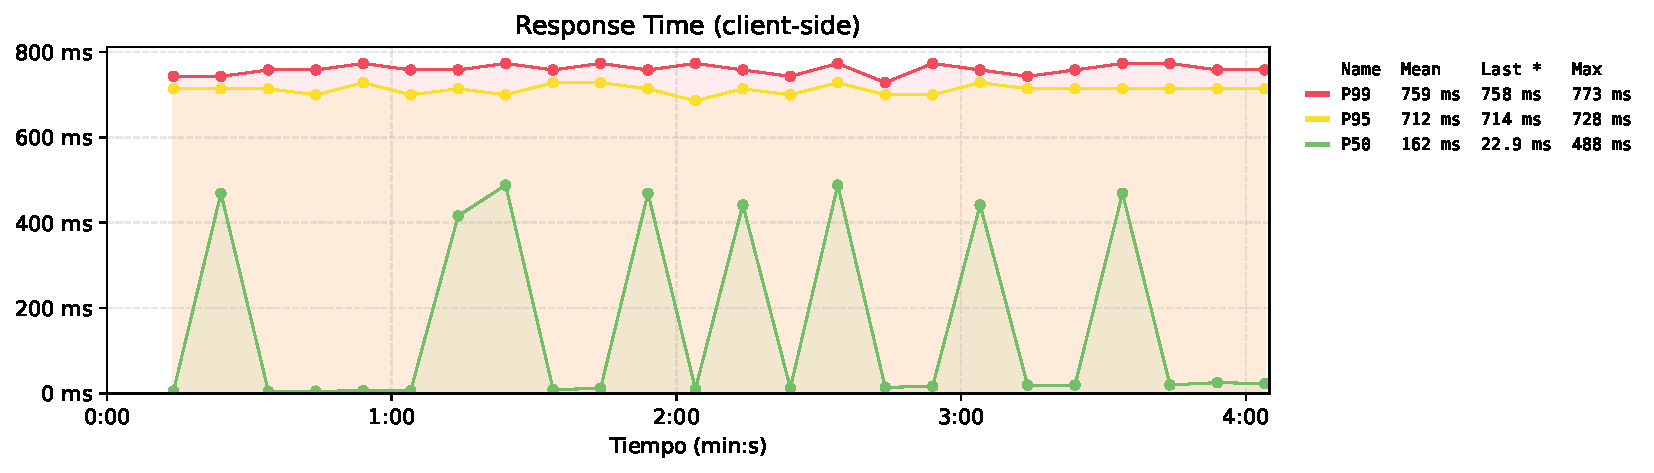
\includegraphics[width=0.8\columnwidth]{figures/sistema_base/baseline/response_time}
            \caption{ Tiempo de respuesta del sistema base. }
            \label{fig:resultados_completos_sistema_base_baseline_response_time}
        \end{figure}

        \begin{figure}[H]
            \centering
            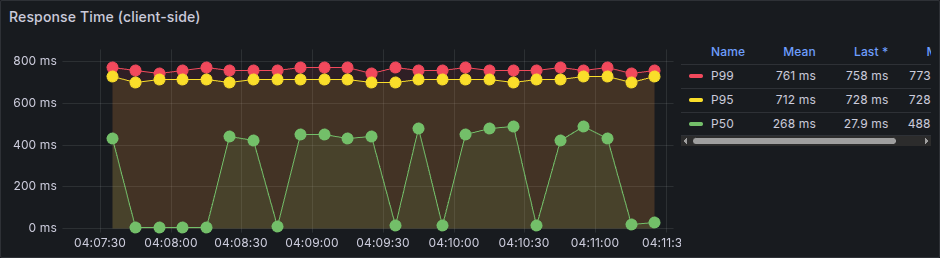
\includegraphics[width=0.8\columnwidth]{figures/sistema_base/baseline/response_time_captura}
            \caption{ Se adjunta la captura correspondiente a la Figura~\ref{fig:resultados_completos_sistema_base_baseline_response_time}. }
            \label{fig:resultados_completos_sistema_base_baseline_response_time_captura}
        \end{figure}

        \begin{figure}[H]
            \centering
            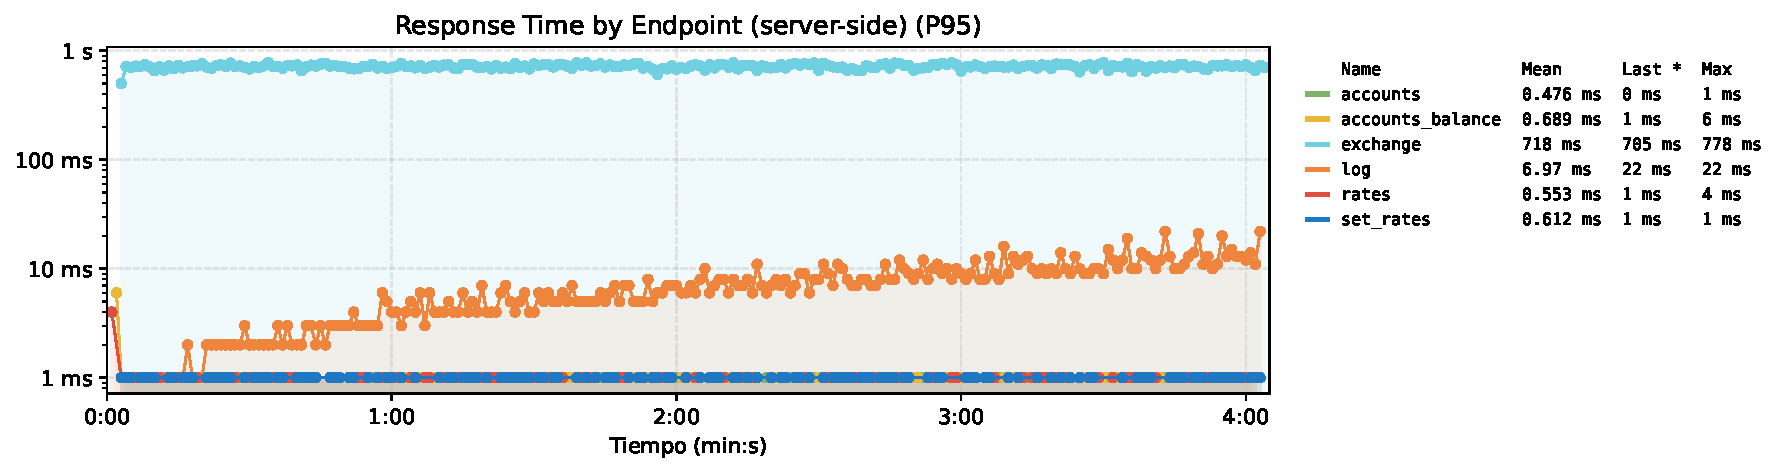
\includegraphics[width=0.8\columnwidth]{figures/sistema_base/baseline/endpoint_response_time}
            \caption{
                Tiempo de respuesta por endpoint del sistema base.
                El eje tiene una escala logarítmica.
            }
            \label{fig:resultados_completos_sistema_base_baseline_endpoint_response_time}
        \end{figure}

        \begin{figure}[H]
            \centering
            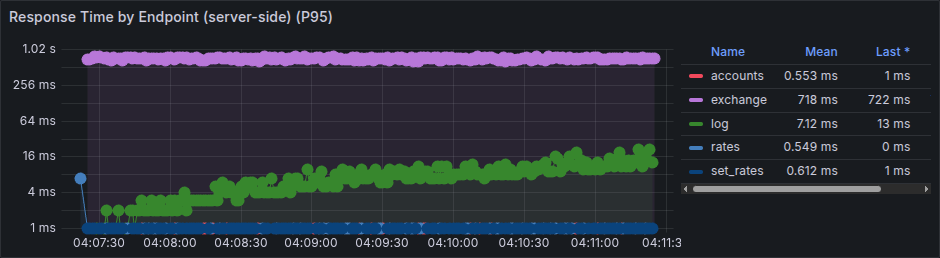
\includegraphics[width=0.8\columnwidth]{figures/sistema_base/baseline/endpoint_response_time_captura}
            \caption{ Se adjunta la captura correspondiente a la Figura~\ref{fig:resultados_completos_sistema_base_baseline_endpoint_response_time}. }
            \label{fig:resultados_completos_sistema_base_baseline_endpoint_response_time_captura}
        \end{figure}

        \begin{figure}[H]
            \centering
            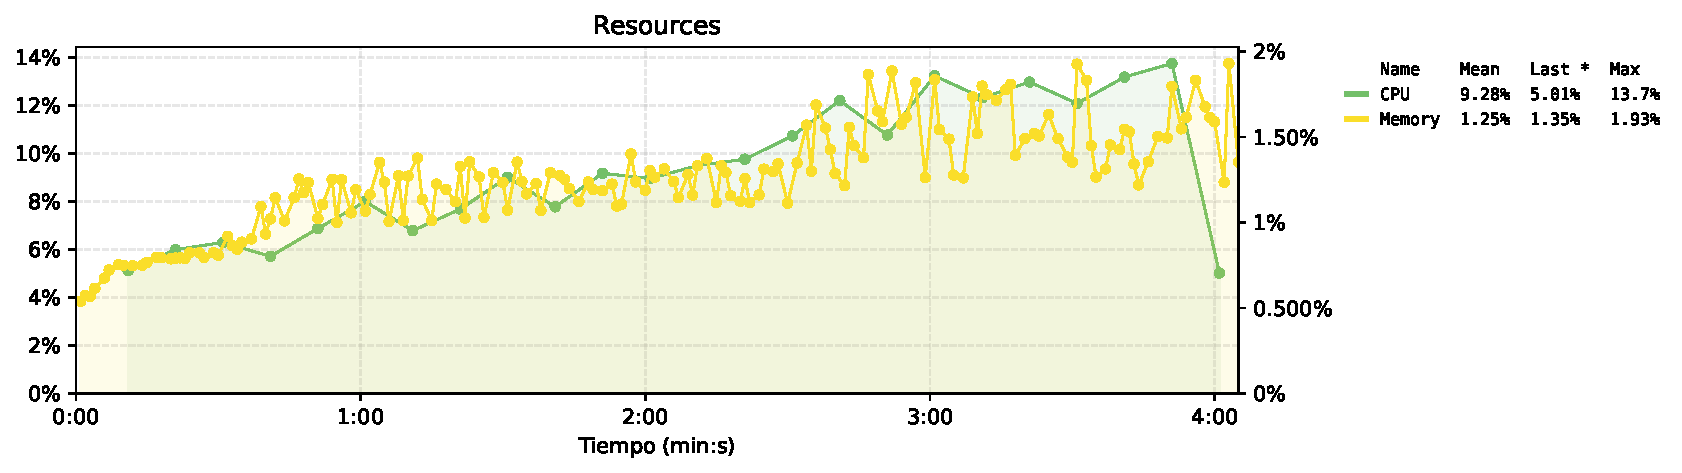
\includegraphics[width=0.8\columnwidth]{figures/sistema_base/baseline/resources}
            \caption{
                Estado de los recursos del sistema base.
                El eje izquierdo muestra el uso de CPU, el eje derecho muestra el uso de memoria.
            }
            \label{fig:resultados_completos_sistema_base_baseline_resources}
        \end{figure}

        \begin{figure}[H]
            \centering
            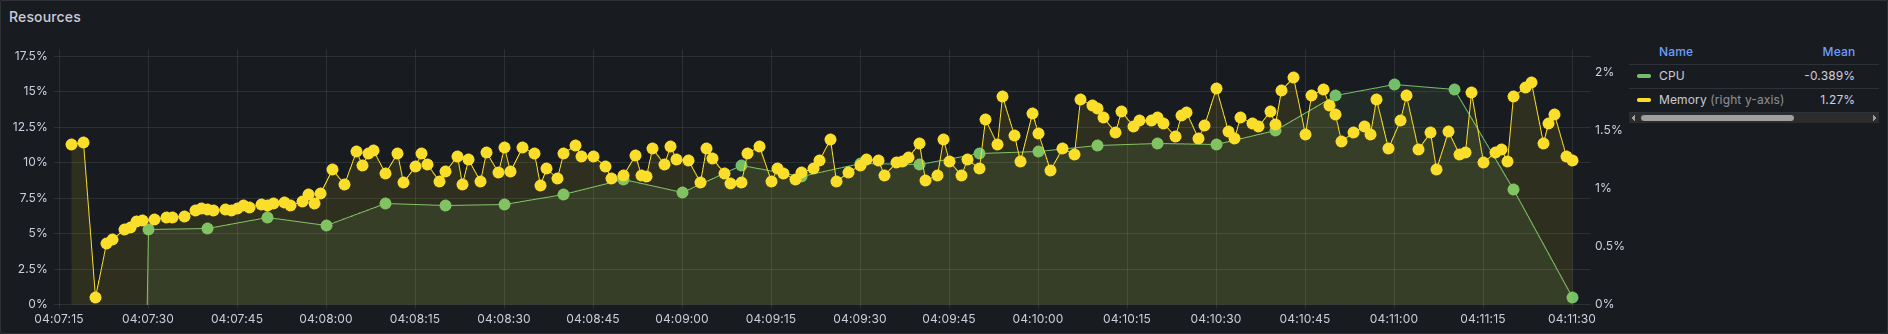
\includegraphics[width=0.8\columnwidth]{figures/sistema_base/baseline/resources_captura}
            \caption{ Se adjunta la captura correspondiente a la Figura~\ref{fig:resultados_completos_sistema_base_baseline_resources}. }
            \label{fig:resultados_completos_sistema_base_baseline_resources_captura}
        \end{figure}

        \begin{figure}[H]
            \centering
            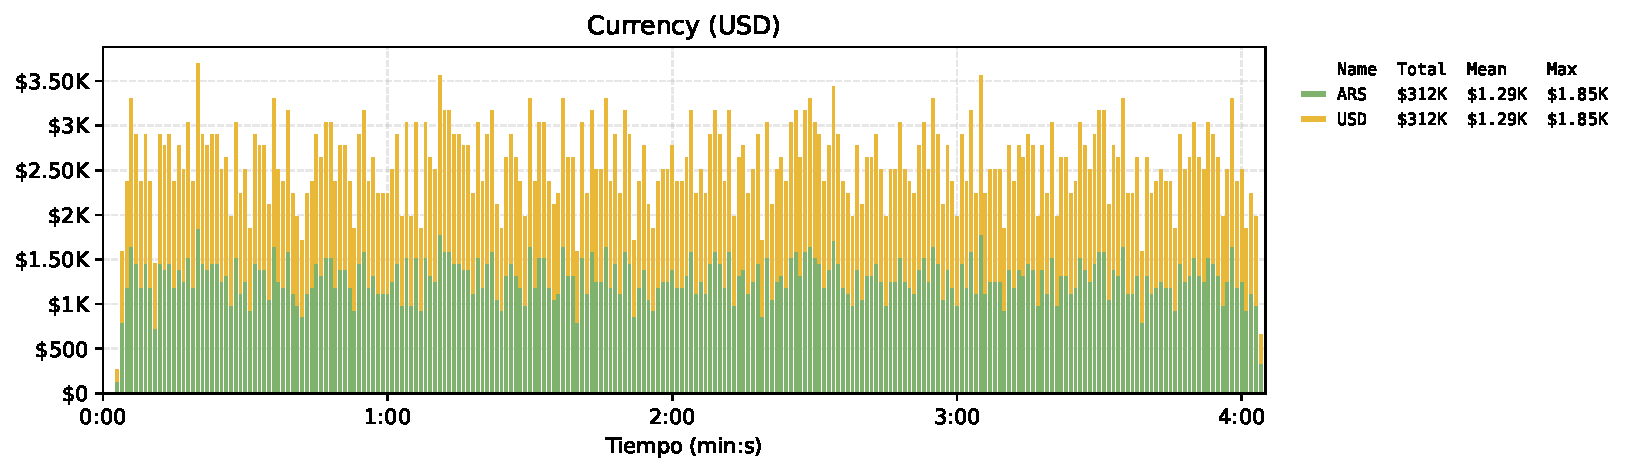
\includegraphics[width=0.8\columnwidth]{figures/sistema_base/baseline/currency}
            \caption{ Volumen operado en cada moneda en el sistema base. }
            \label{fig:resultados_completos_sistema_base_baseline_currency}
        \end{figure}

        \begin{figure}[H]
            \centering
            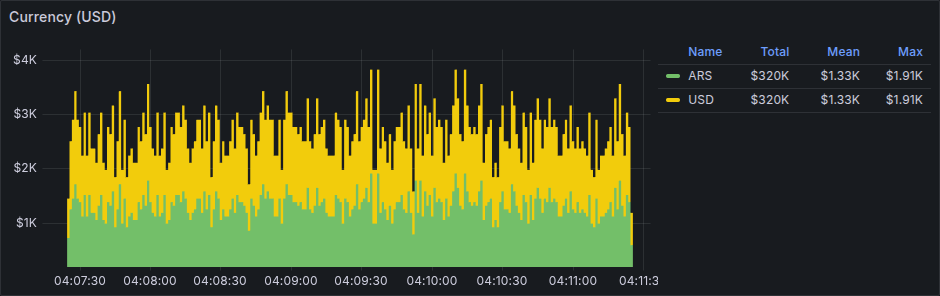
\includegraphics[width=0.8\columnwidth]{figures/sistema_base/baseline/currency_captura}
            \caption{ Se adjunta la captura correspondiente a la Figura~\ref{fig:resultados_completos_sistema_base_baseline_currency}. }
            \label{fig:resultados_completos_sistema_base_baseline_currency_captura}
        \end{figure}

        \begin{figure}[H]
            \centering
            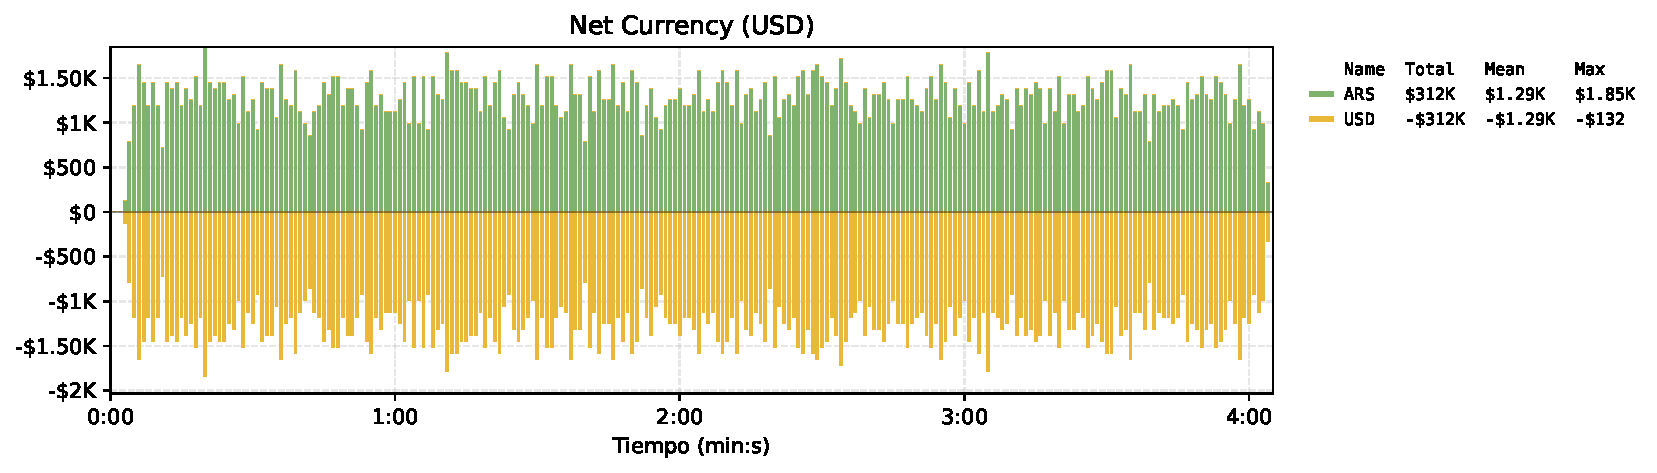
\includegraphics[width=0.8\columnwidth]{figures/sistema_base/baseline/net_currency}
            \caption{ Neto operado en cada moneda en el sistema base. }
            \label{fig:resultados_completos_sistema_base_baseline_net_currency}
        \end{figure}

        \begin{figure}[H]
            \centering
            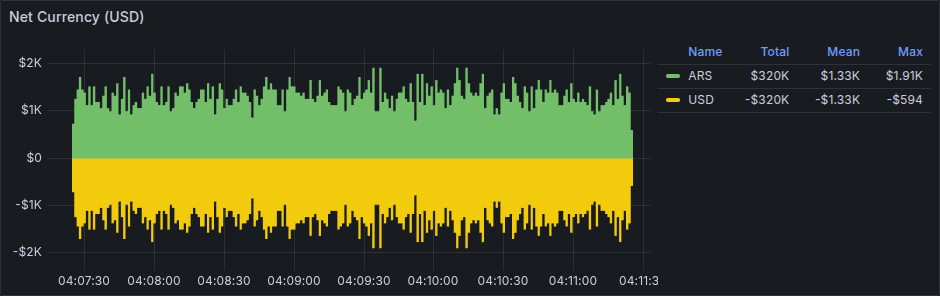
\includegraphics[width=0.8\columnwidth]{figures/sistema_base/baseline/net_currency_captura}
            \caption{ Se adjunta la captura correspondiente a la Figura~\ref{fig:resultados_completos_sistema_base_baseline_net_currency}. }
            \label{fig:resultados_completos_sistema_base_baseline_net_currency_captura}
        \end{figure}

    \clearpage

    \subsection{Resultados completos del escenario de estrés sobre el sistema base}
    \label{sec:resultados_completos_sistema_base_stress}

        \begin{figure}[H]
            \centering
            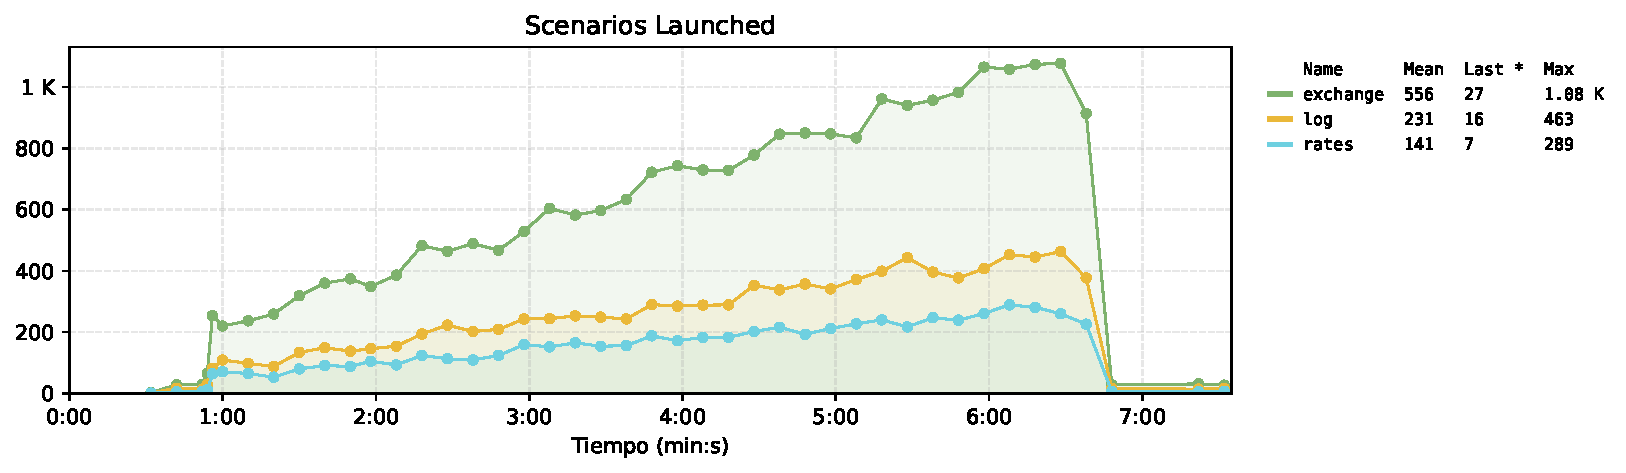
\includegraphics[width=0.8\columnwidth]{figures/sistema_base/stress/scenarios}
            \caption{ Escenarios del sistema base. }
            \label{fig:resultados_completos_sistema_base_stress_scenarios}
        \end{figure}

        \begin{figure}[H]
            \centering
            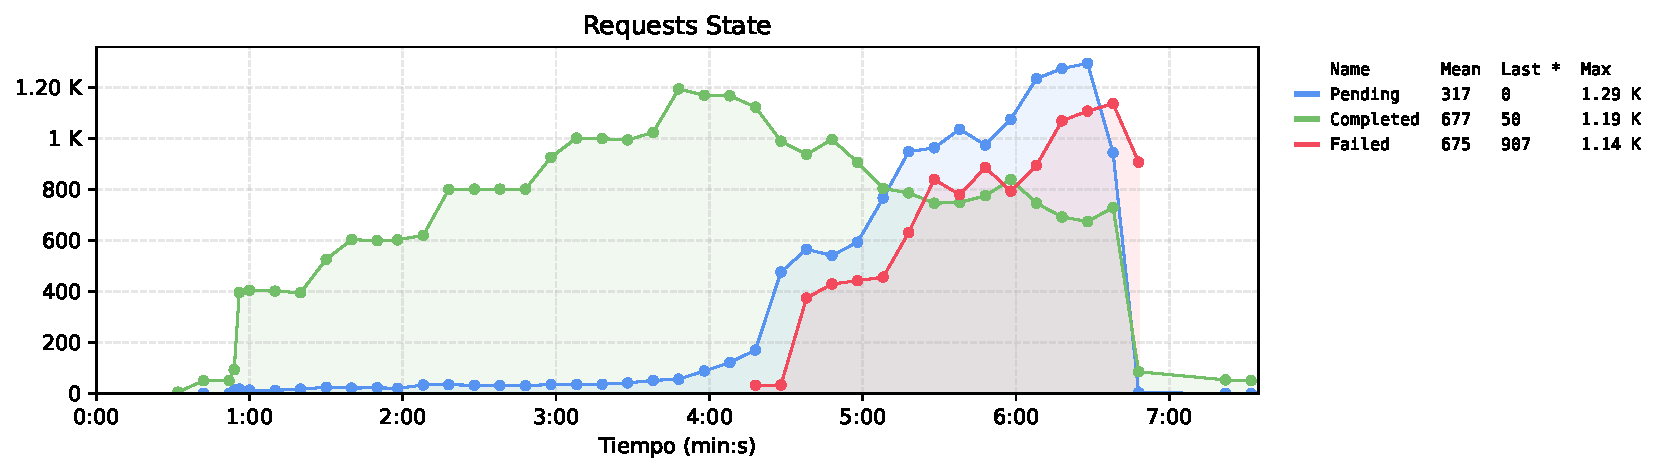
\includegraphics[width=0.8\columnwidth]{figures/sistema_base/stress/requests_state}
            \caption{ Estado de las requests del sistema base. }
            \label{fig:resultados_completos_sistema_base_stress_requests_state}
        \end{figure}

        \begin{figure}[H]
            \centering
            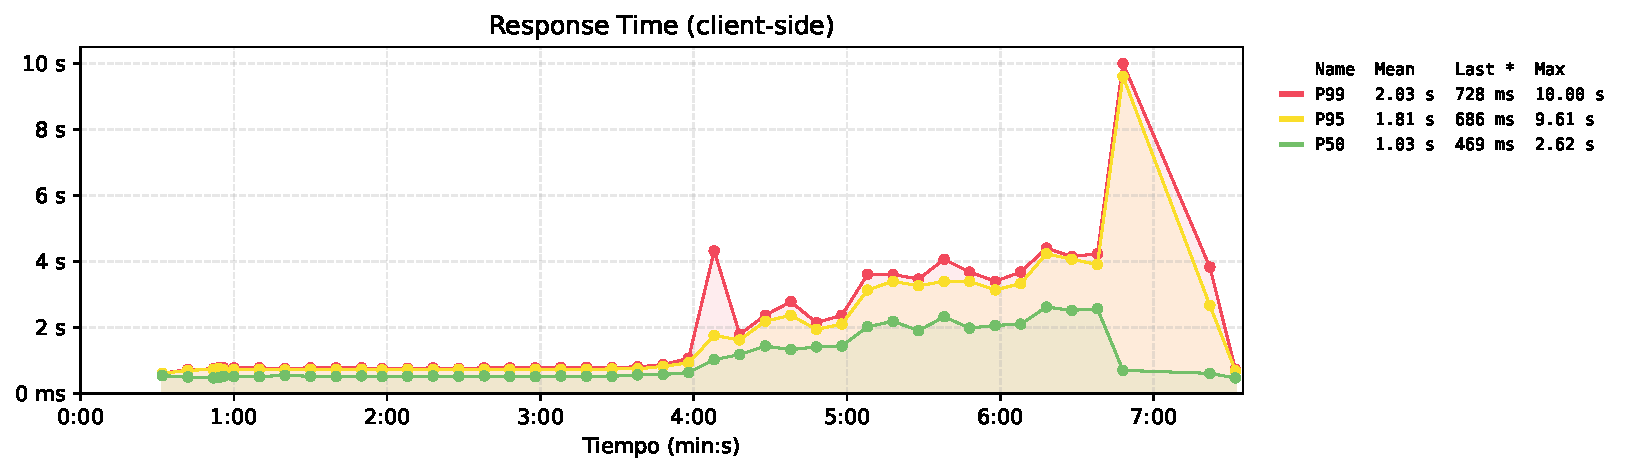
\includegraphics[width=0.8\columnwidth]{figures/sistema_base/stress/response_time}
            \caption{ Tiempo de respuesta del sistema base. }
            \label{fig:resultados_completos_sistema_base_stress_response_time}
        \end{figure}

        \begin{figure}[H]
            \centering
            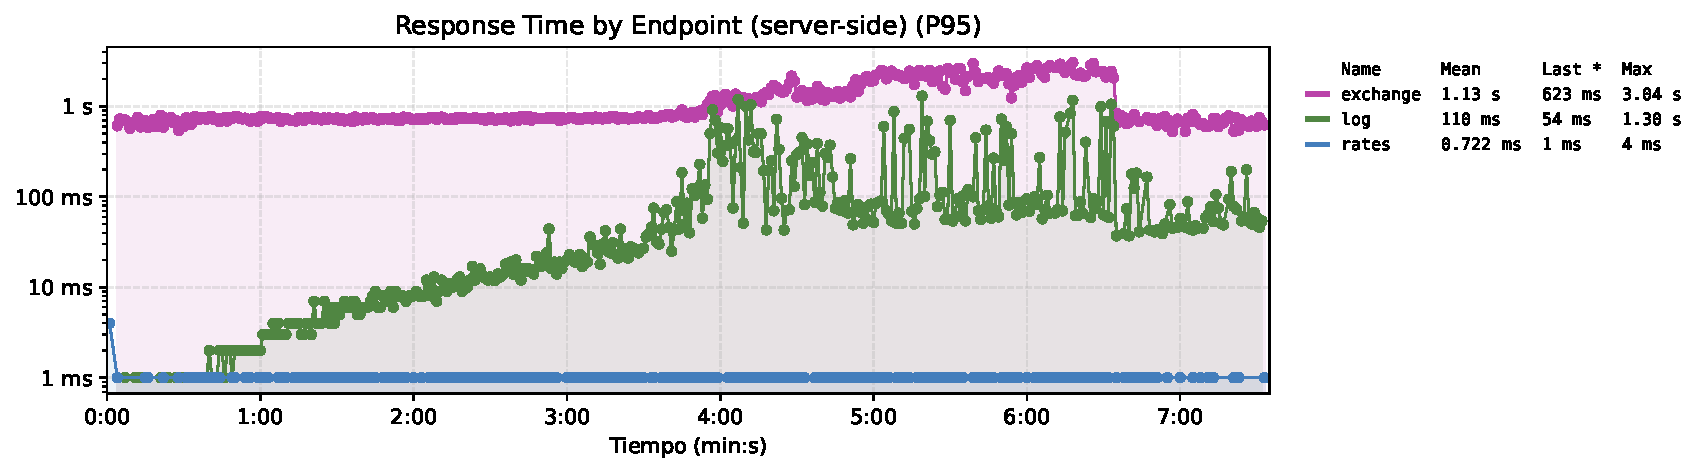
\includegraphics[width=0.8\columnwidth]{figures/sistema_base/stress/endpoint_response_time}
            \caption{
                Tiempo de respuesta por endpoint del sistema base.
                El eje tiene una escala logarítmica.
            }
            \label{fig:resultados_completos_sistema_base_stress_endpoint_response_time}
        \end{figure}

        \begin{figure}[H]
            \centering
            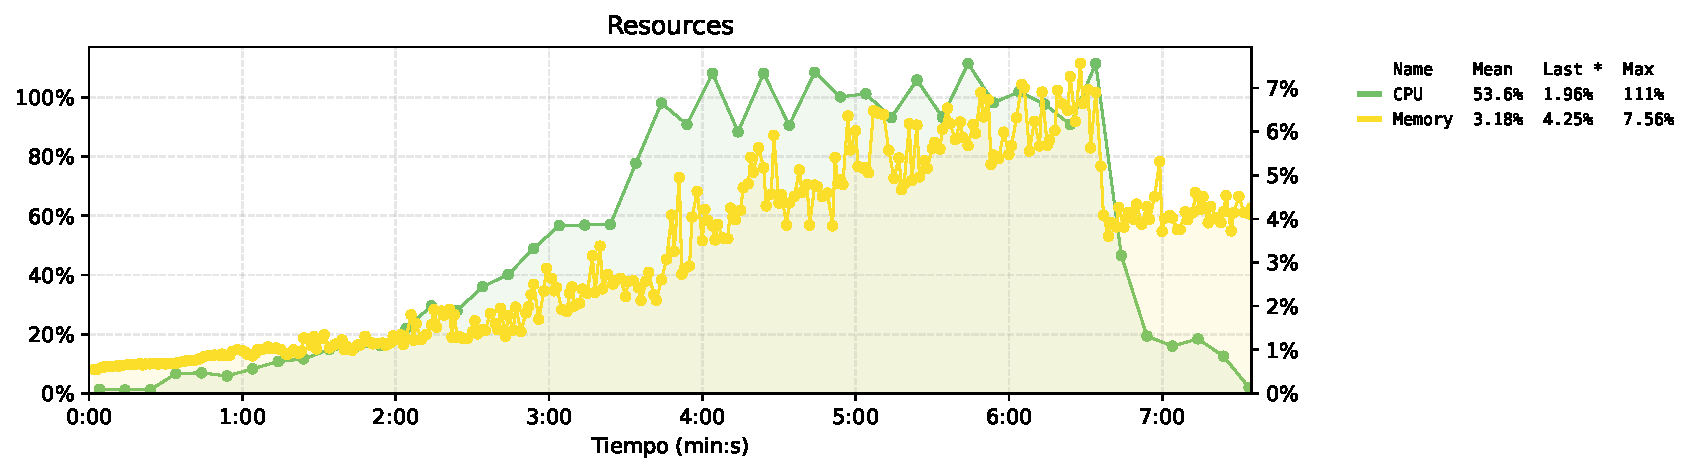
\includegraphics[width=0.8\columnwidth]{figures/sistema_base/stress/resources}
            \caption{
                Estado de los recursos del sistema base.
                El eje izquierdo muestra el uso de CPU, el eje derecho muestra el uso de memoria.
            }
            \label{fig:resultados_completos_sistema_base_stress_resources}
        \end{figure}

        \begin{figure}[H]
            \centering
            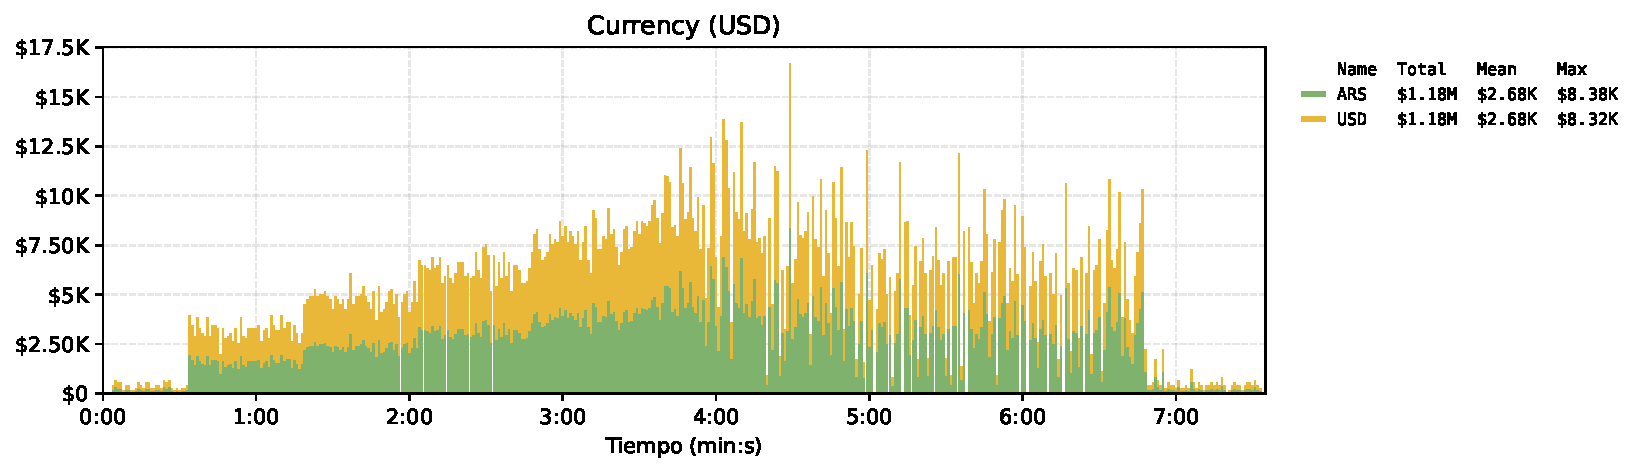
\includegraphics[width=0.8\columnwidth]{figures/sistema_base/stress/currency}
            \caption{ Volumen operado en cada moneda en el sistema base. }
            \label{fig:resultados_completos_sistema_base_stress_currency}
        \end{figure}

        \begin{figure}[H]
            \centering
            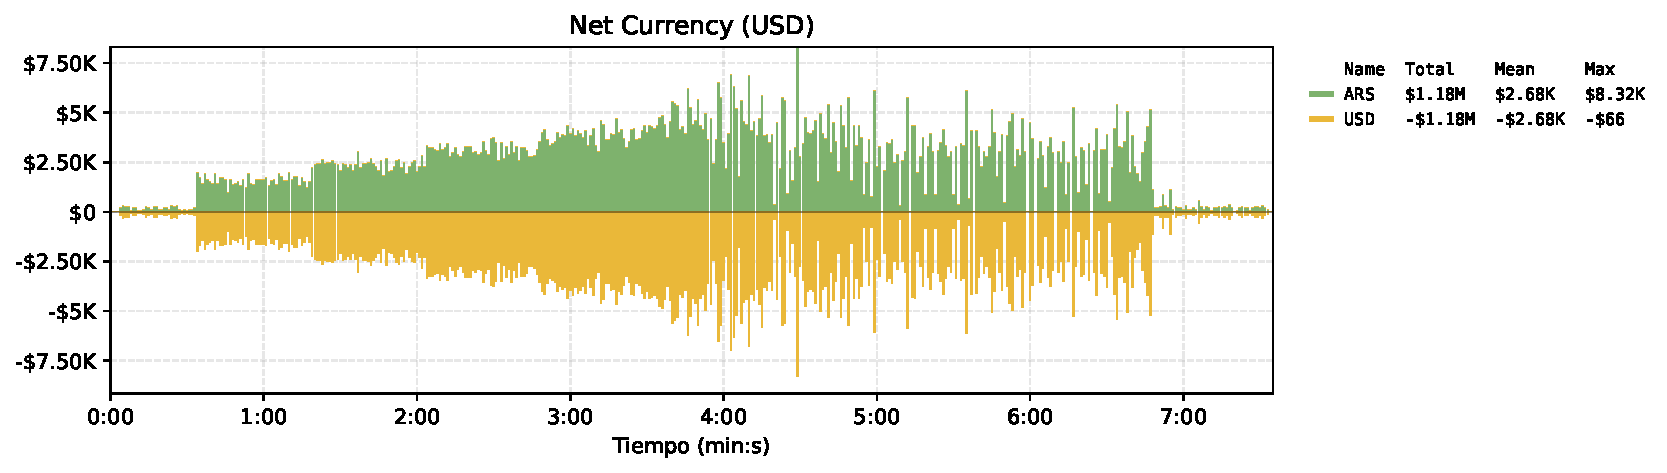
\includegraphics[width=0.8\columnwidth]{figures/sistema_base/stress/net_currency}
            \caption{ Neto operado en cada moneda en el sistema base. }
            \label{fig:resultados_completos_sistema_base_stress_net_currency}
        \end{figure}

    \clearpage

    \subsection{Resultados completos del escenario de resistencia sobre el sistema base}
    \label{sec:resultados_completos_sistema_base_soak}

        \begin{figure}[H]
            \centering
            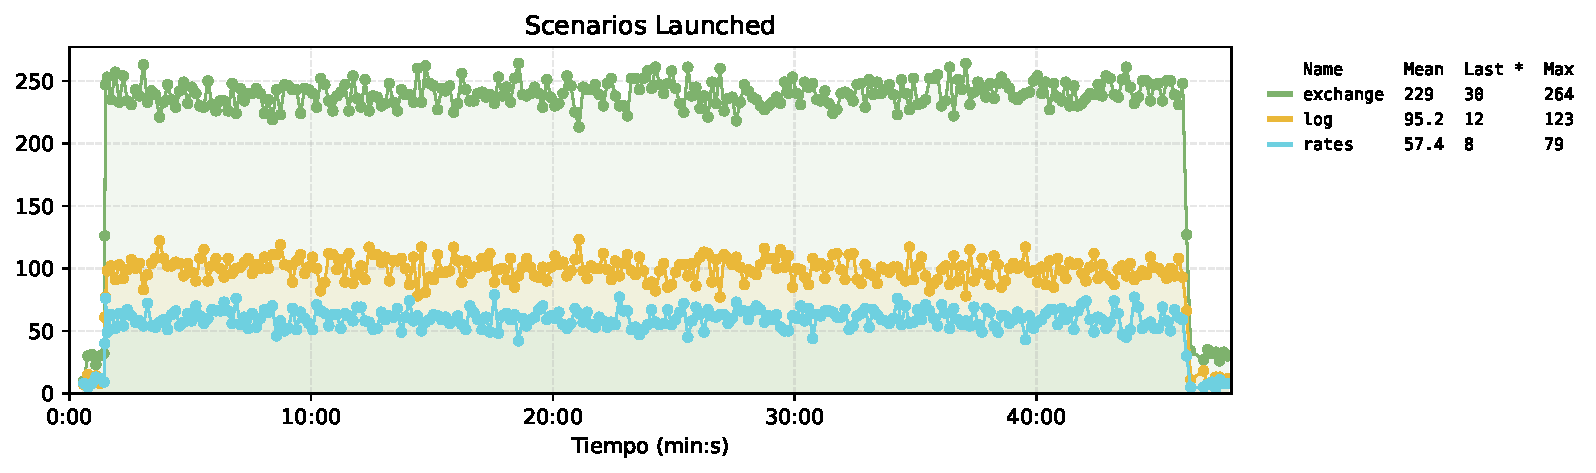
\includegraphics[width=0.8\columnwidth]{figures/sistema_base/soak/scenarios}
            \caption{ Escenarios del sistema base. }
            \label{fig:resultados_completos_sistema_base_soak_scenarios}
        \end{figure}

        \begin{figure}[H]
            \centering
            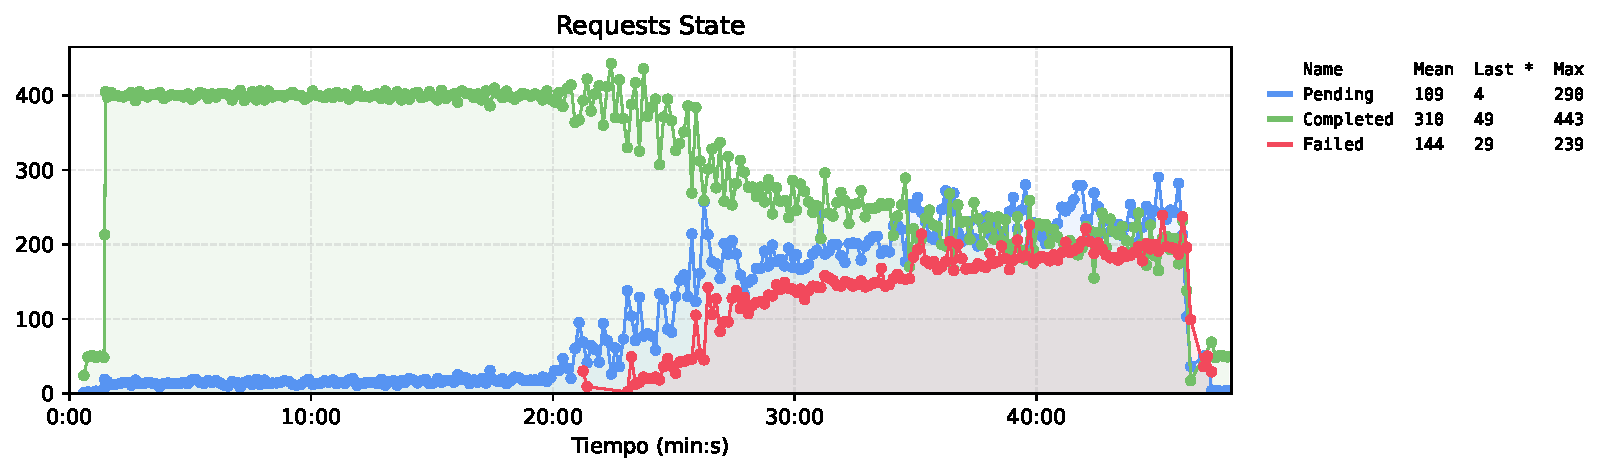
\includegraphics[width=0.8\columnwidth]{figures/sistema_base/soak/requests_state}
            \caption{ Estado de las requests del sistema base. }
            \label{fig:resultados_completos_sistema_base_soak_requests_state}
        \end{figure}

        \begin{figure}[H]
            \centering
            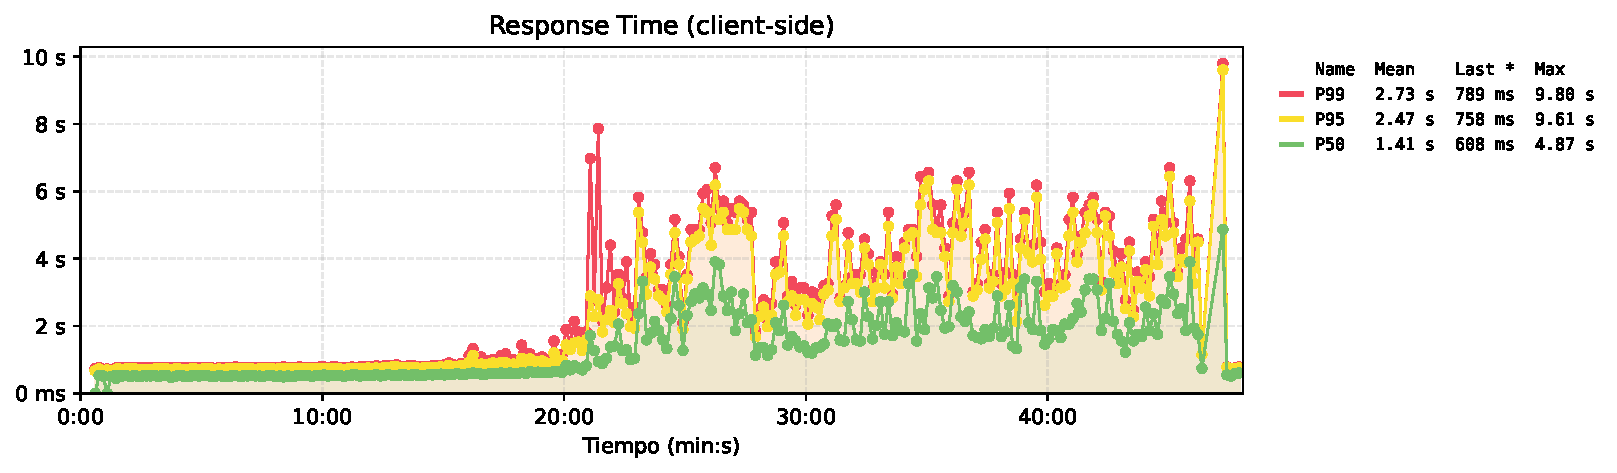
\includegraphics[width=0.8\columnwidth]{figures/sistema_base/soak/response_time}
            \caption{ Tiempo de respuesta del sistema base. }
            \label{fig:resultados_completos_sistema_base_soak_response_time}
        \end{figure}

        \begin{figure}[H]
            \centering
            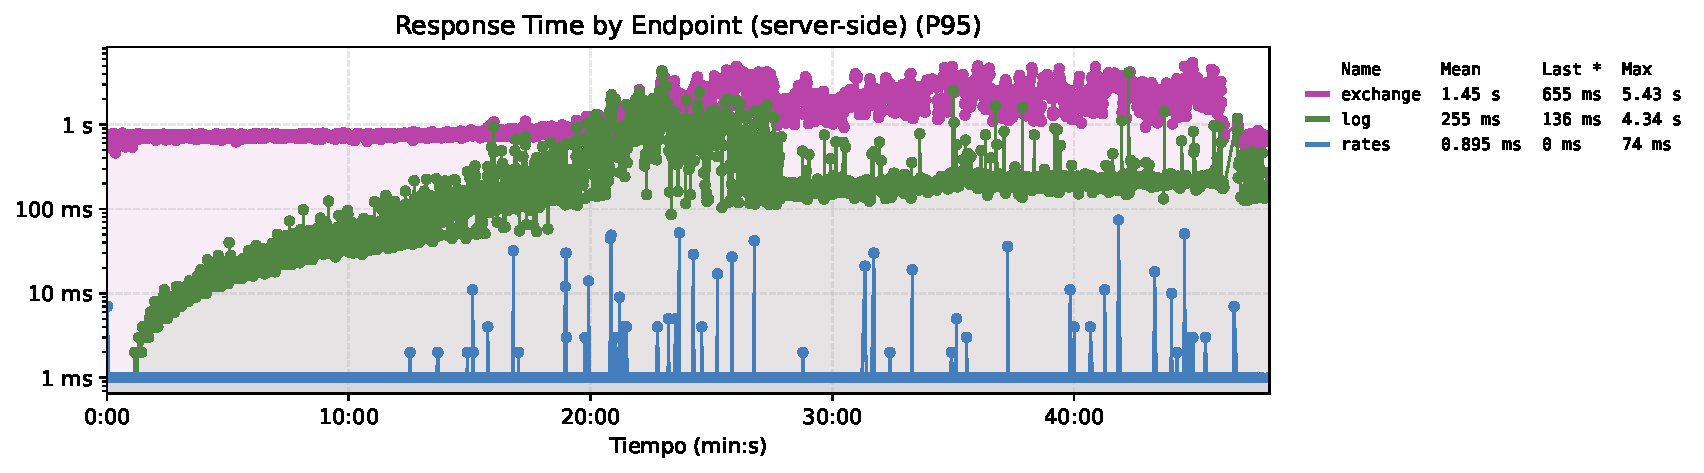
\includegraphics[width=0.8\columnwidth]{figures/sistema_base/soak/endpoint_response_time}
            \caption{
                Tiempo de respuesta por endpoint del sistema base.
                El eje tiene una escala logarítmica.
            }
            \label{fig:resultados_completos_sistema_base_soak_endpoint_response_time}
        \end{figure}

        \begin{figure}[H]
            \centering
            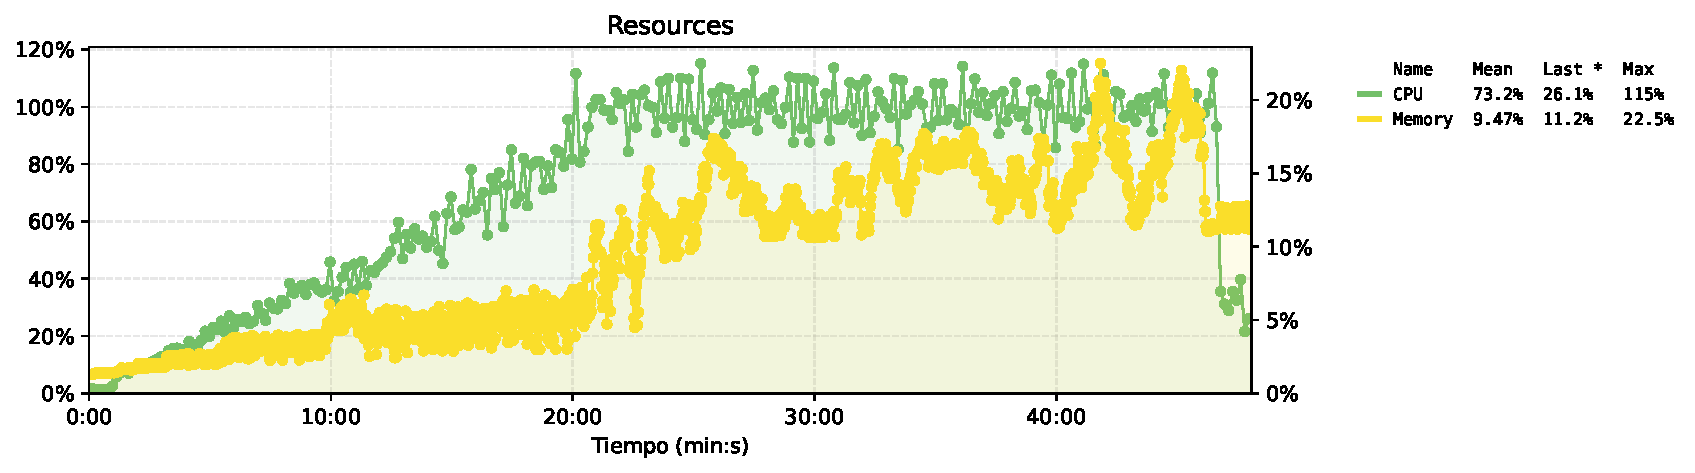
\includegraphics[width=0.8\columnwidth]{figures/sistema_base/soak/resources}
            \caption{
                Estado de los recursos del sistema base.
                El eje izquierdo muestra el uso de CPU, el eje derecho muestra el uso de memoria.
            }
            \label{fig:resultados_completos_sistema_base_soak_resources}
        \end{figure}

        \begin{figure}[H]
            \centering
            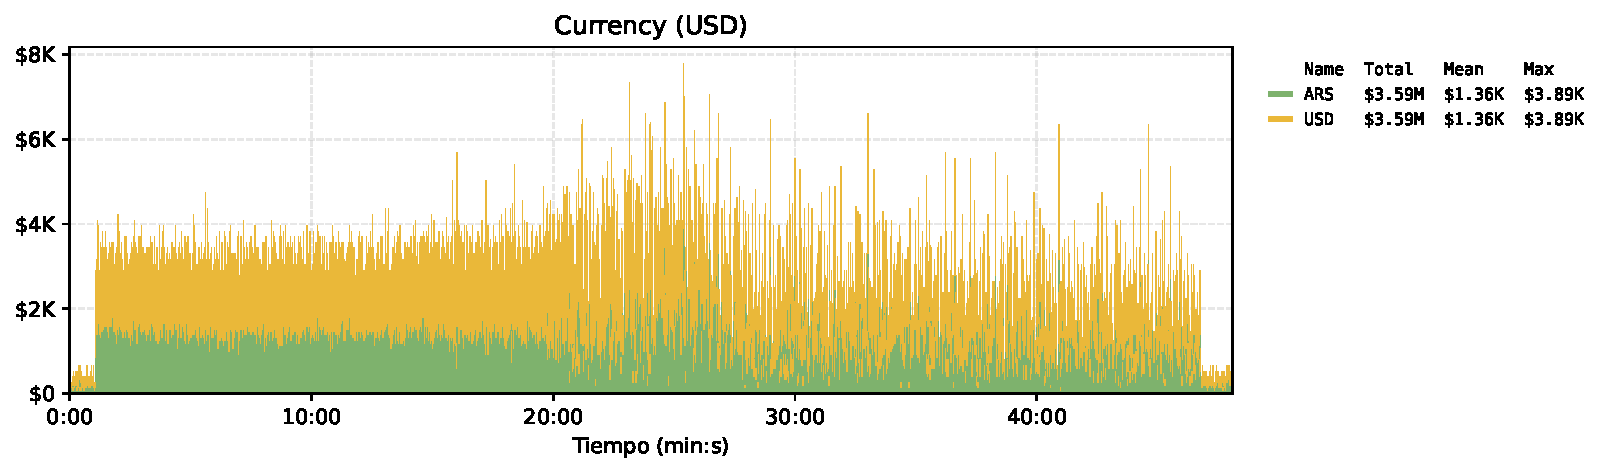
\includegraphics[width=0.8\columnwidth]{figures/sistema_base/soak/currency}
            \caption{ Volumen operado en cada moneda en el sistema base. }
            \label{fig:resultados_completos_sistema_base_soak_currency}
        \end{figure}

        \begin{figure}[H]
            \centering
            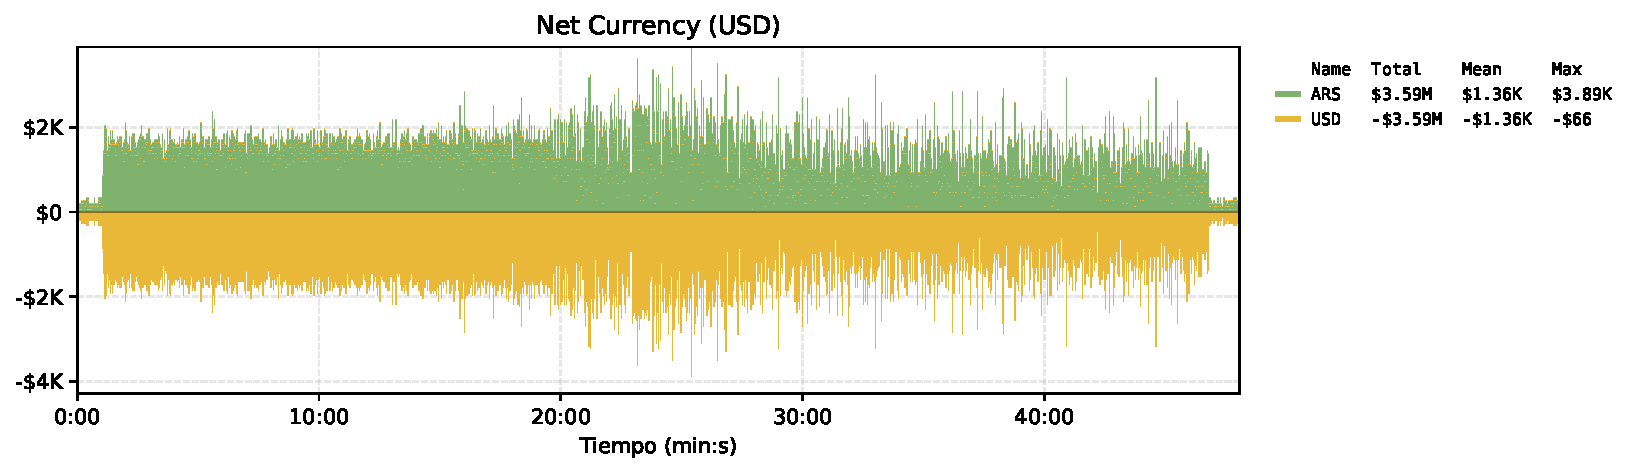
\includegraphics[width=0.8\columnwidth]{figures/sistema_base/soak/net_currency}
            \caption{ Neto operado en cada moneda en el sistema base. }
            \label{fig:resultados_completos_sistema_base_soak_net_currency}
        \end{figure}

    \clearpage

    \subsection{Resultados completos del escenario de caos sobre el sistema base}
    \label{sec:resultados_completos_sistema_base_chaos}

        \begin{figure}[H]
            \centering
            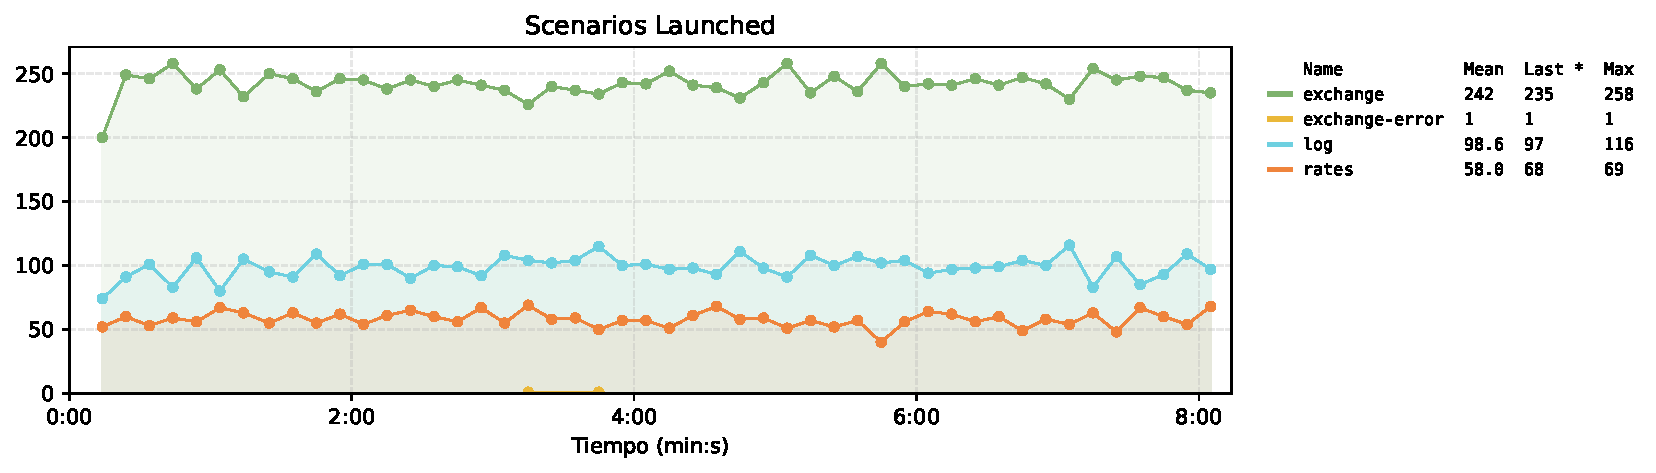
\includegraphics[width=0.8\columnwidth]{figures/sistema_base/chaos/scenarios}
            \caption{ Escenarios del sistema base. }
            \label{fig:resultados_completos_sistema_base_chaos_scenarios}
        \end{figure}

        \begin{figure}[H]
            \centering
            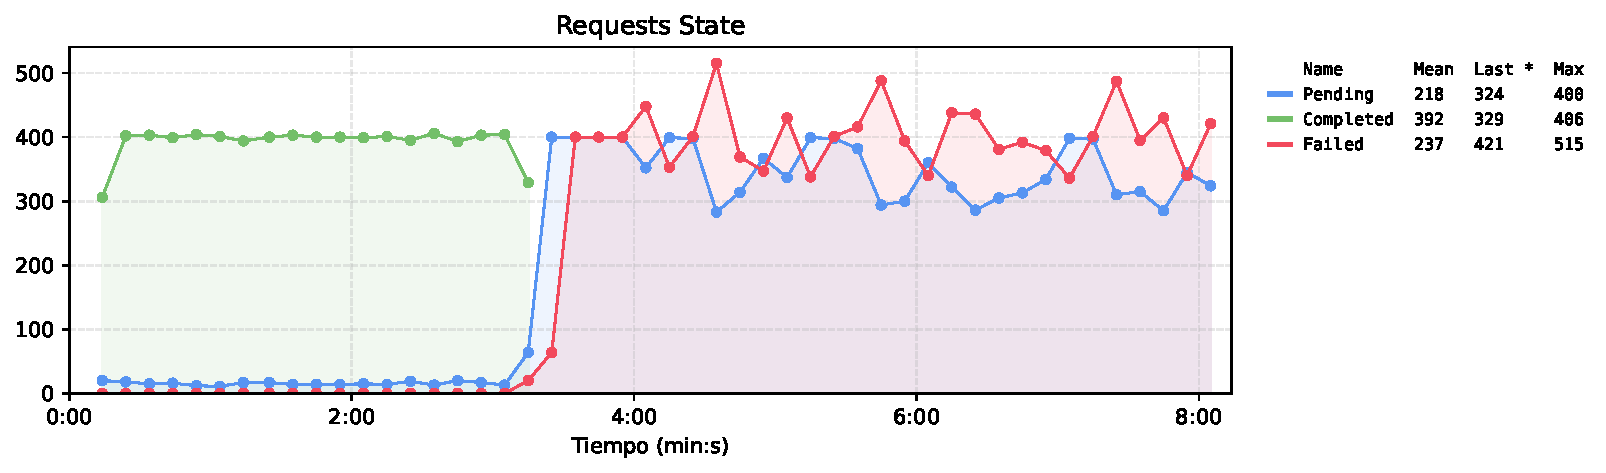
\includegraphics[width=0.8\columnwidth]{figures/sistema_base/chaos/requests_state}
            \caption{ Estado de las requests del sistema base. }
            \label{fig:resultados_completos_sistema_base_chaos_requests_state}
        \end{figure}

        \begin{figure}[H]
            \centering
            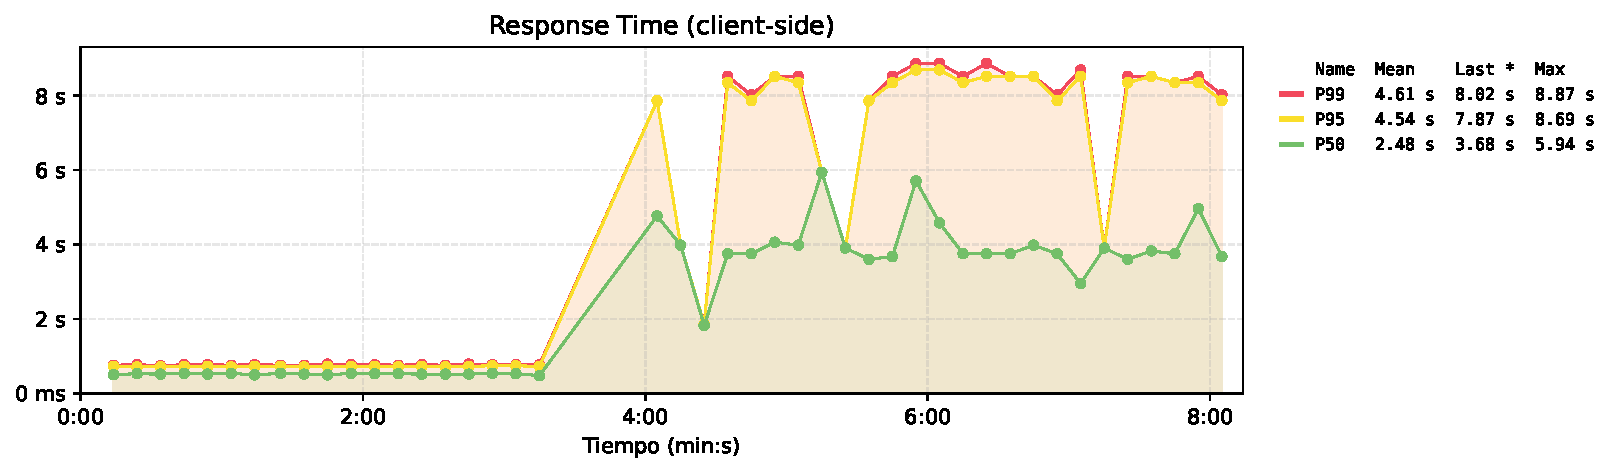
\includegraphics[width=0.8\columnwidth]{figures/sistema_base/chaos/response_time}
            \caption{ Tiempo de respuesta del sistema base. }
            \label{fig:resultados_completos_sistema_base_chaos_response_time}
        \end{figure}

        \begin{figure}[H]
            \centering
            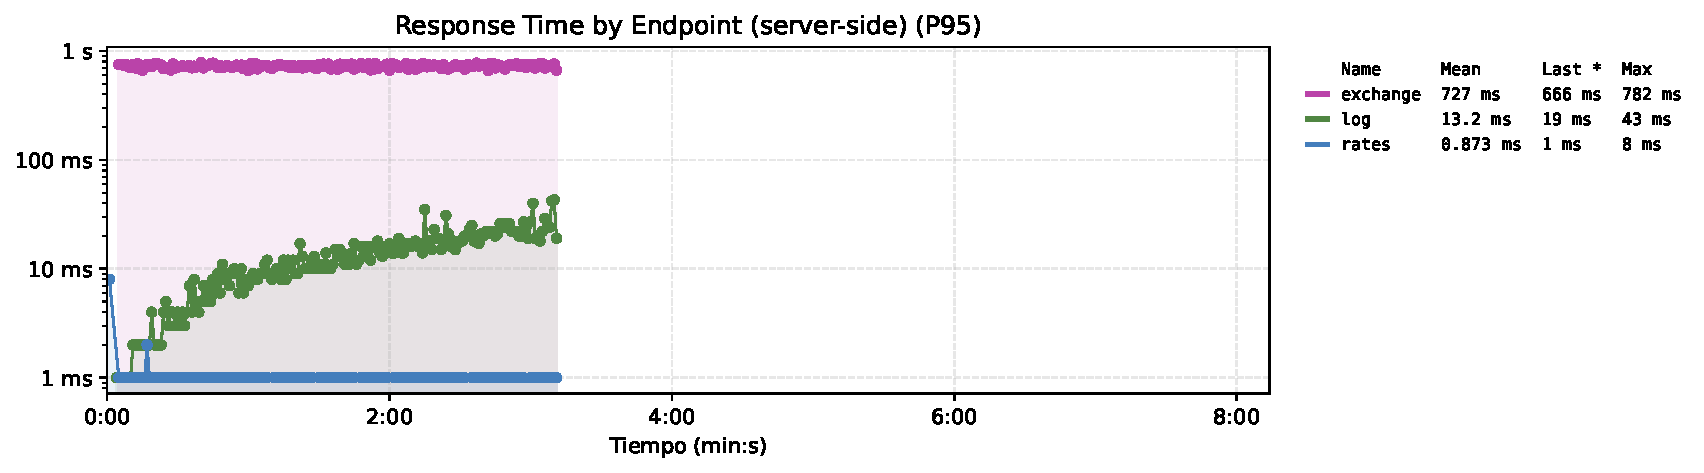
\includegraphics[width=0.8\columnwidth]{figures/sistema_base/chaos/endpoint_response_time}
            \caption{
                Tiempo de respuesta por endpoint del sistema base.
                El eje tiene una escala logarítmica.
            }
            \label{fig:resultados_completos_sistema_base_chaos_endpoint_response_time}
        \end{figure}

        \begin{figure}[H]
            \centering
            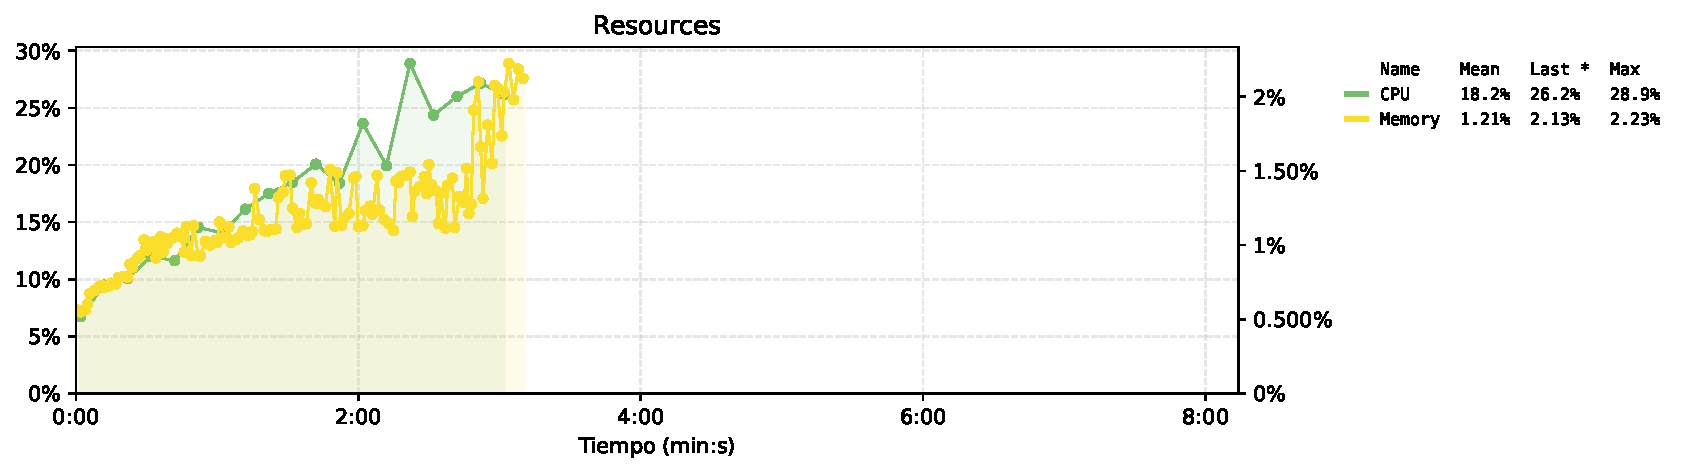
\includegraphics[width=0.8\columnwidth]{figures/sistema_base/chaos/resources}
            \caption{
                Estado de los recursos del sistema base.
                El eje izquierdo muestra el uso de CPU, el eje derecho muestra el uso de memoria.
            }
            \label{fig:resultados_completos_sistema_base_chaos_resources}
        \end{figure}

        \begin{figure}[H]
            \centering
            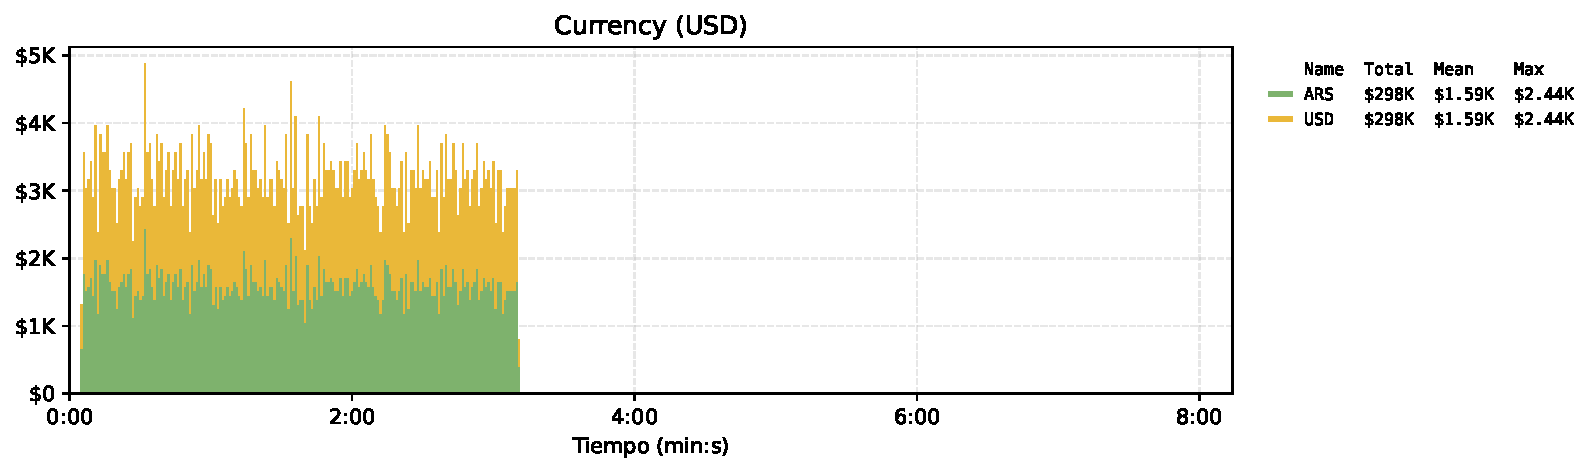
\includegraphics[width=0.8\columnwidth]{figures/sistema_base/chaos/currency}
            \caption{ Volumen operado en cada moneda en el sistema base. }
            \label{fig:resultados_completos_sistema_base_chaos_currency}
        \end{figure}

        \begin{figure}[H]
            \centering
            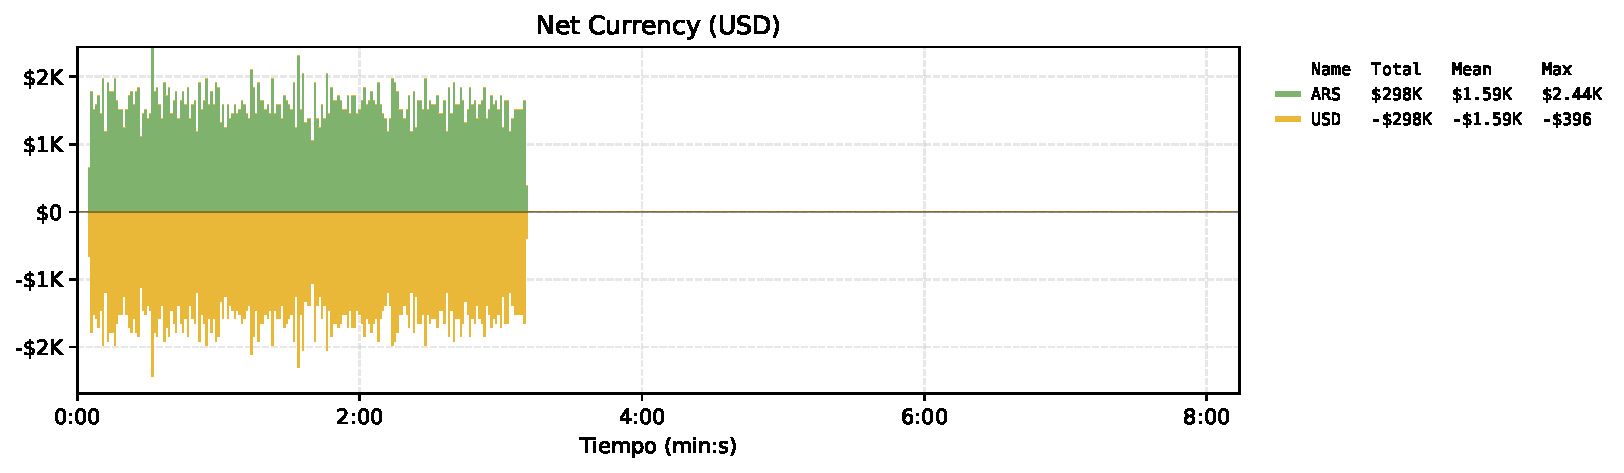
\includegraphics[width=0.8\columnwidth]{figures/sistema_base/chaos/net_currency}
            \caption{ Neto operado en cada moneda en el sistema base. }
            \label{fig:resultados_completos_sistema_base_chaos_net_currency}
        \end{figure}

    \clearpage

    \subsection{Resultados completos del escenario de concurrencia sobre el sistema base}
    \label{sec:resultados_completos_sistema_base_race}

        \begin{figure}[H]
            \centering
            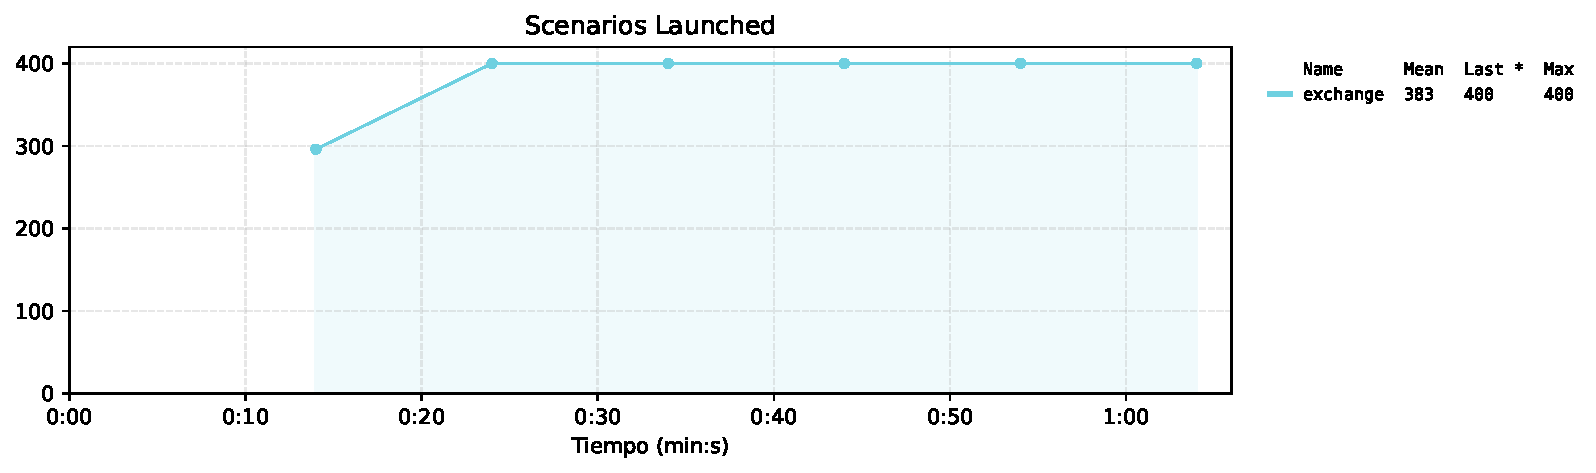
\includegraphics[width=0.8\columnwidth]{figures/sistema_base/race/scenarios}
            \caption{ Escenarios del sistema base. }
            \label{fig:resultados_completos_sistema_base_race_scenarios}
        \end{figure}

        \begin{figure}[H]
            \centering
            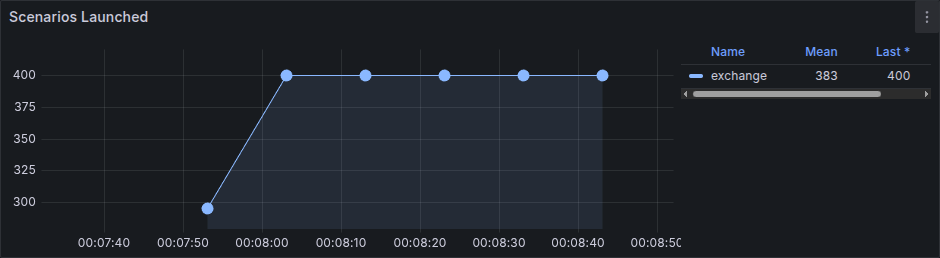
\includegraphics[width=0.8\columnwidth]{figures/sistema_base/race/scenarios_captura}
            \caption{ Se adjunta la captura correspondiente a la Figura~\ref{fig:resultados_completos_sistema_base_race_scenarios}. }
            \label{fig:resultados_completos_sistema_base_race_scenarios_captura}
        \end{figure}

        \begin{figure}[H]
            \centering
            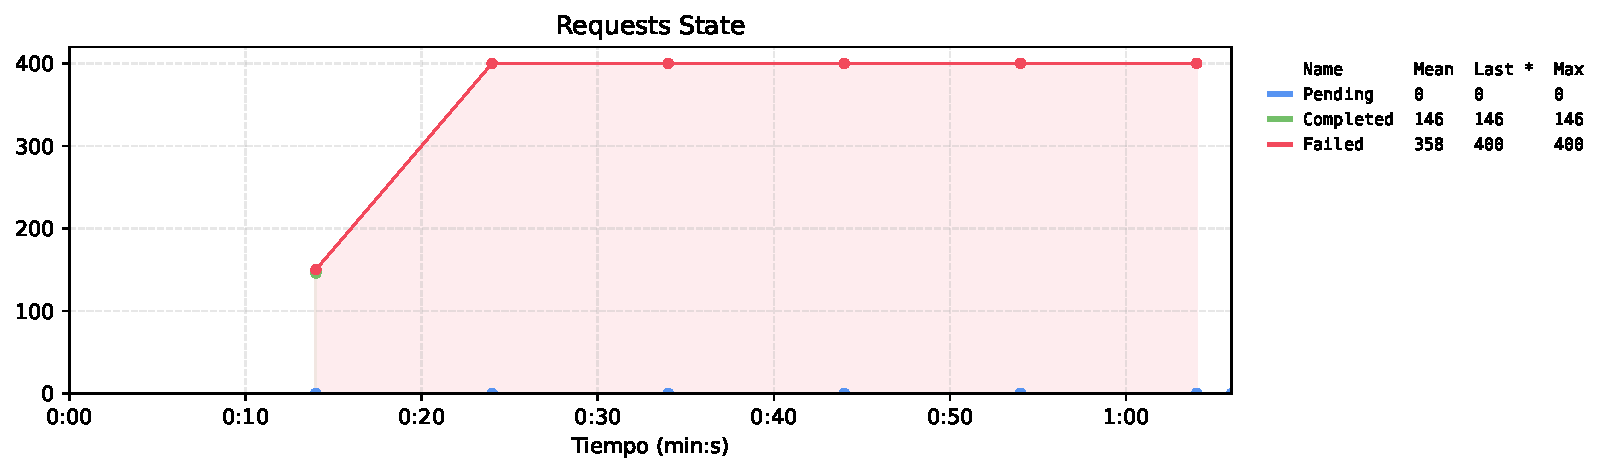
\includegraphics[width=0.8\columnwidth]{figures/sistema_base/race/requests_state}
            \caption{ Estado de las requests del sistema base. }
            \label{fig:resultados_completos_sistema_base_race_requests_state}
        \end{figure}

        \begin{figure}[H]
            \centering
            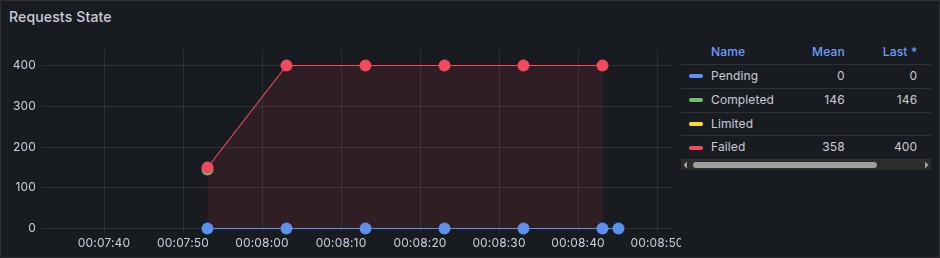
\includegraphics[width=0.8\columnwidth]{figures/sistema_base/race/requests_state_captura}
            \caption{ Se adjunta la captura correspondiente a la Figura~\ref{fig:resultados_completos_sistema_base_race_requests_state}. }
            \label{fig:resultados_completos_sistema_base_race_requests_state_captura}
        \end{figure}

        \begin{figure}[H]
            \centering
            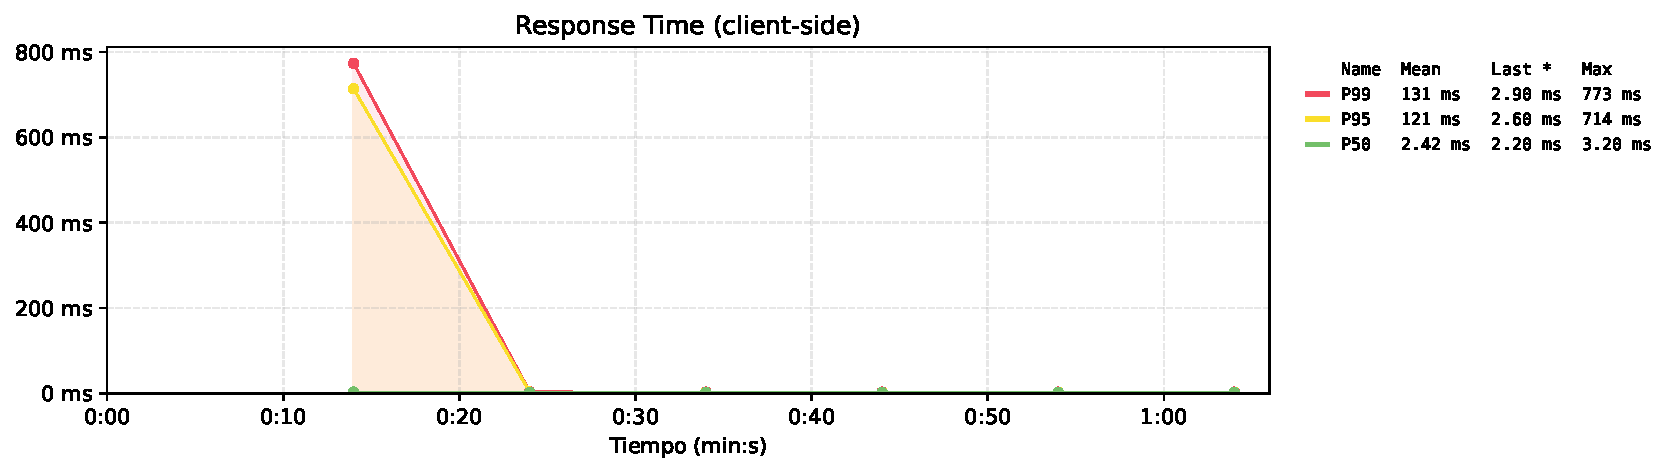
\includegraphics[width=0.8\columnwidth]{figures/sistema_base/race/response_time}
            \caption{ Tiempo de respuesta del sistema base. }
            \label{fig:resultados_completos_sistema_base_race_response_time}
        \end{figure}

        \begin{figure}[H]
            \centering
            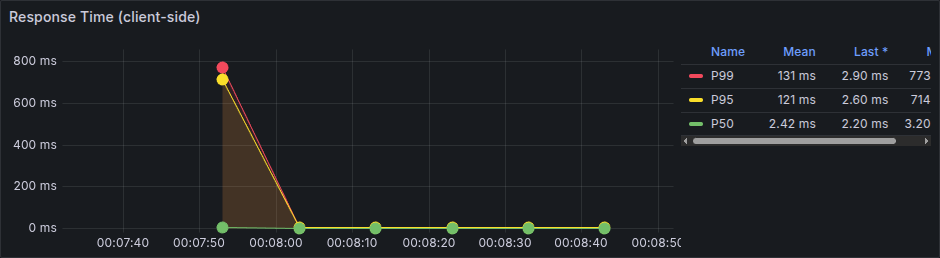
\includegraphics[width=0.8\columnwidth]{figures/sistema_base/race/response_time_captura}
            \caption{ Se adjunta la captura correspondiente a la Figura~\ref{fig:resultados_completos_sistema_base_race_response_time}. }
            \label{fig:resultados_completos_sistema_base_race_response_time_captura}
        \end{figure}

        \begin{figure}[H]
            \centering
            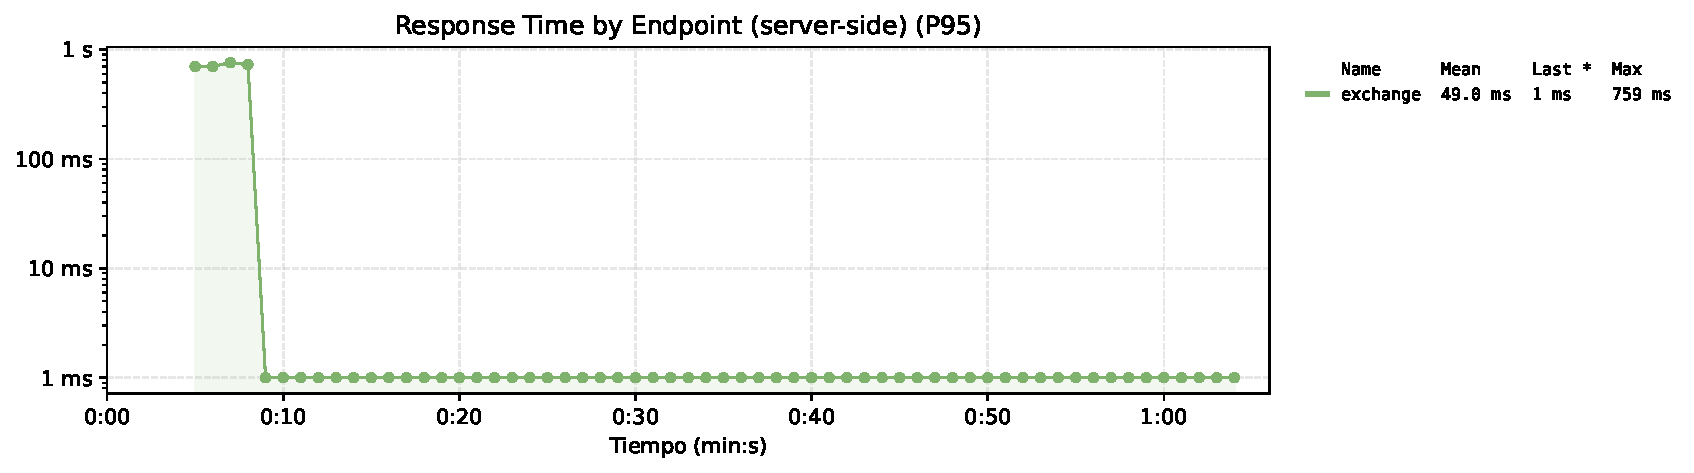
\includegraphics[width=0.8\columnwidth]{figures/sistema_base/race/endpoint_response_time}
            \caption{
                Tiempo de respuesta por endpoint del sistema base.
                El eje tiene una escala logarítmica.
            }
            \label{fig:resultados_completos_sistema_base_race_endpoint_response_time}
        \end{figure}

        \begin{figure}[H]
            \centering
            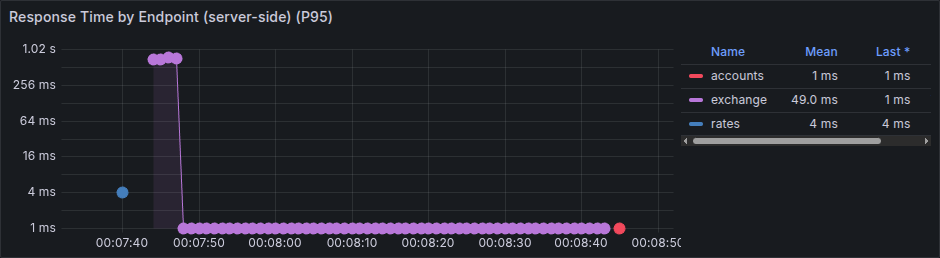
\includegraphics[width=0.8\columnwidth]{figures/sistema_base/race/endpoint_response_time_captura}
            \caption{ Se adjunta la captura correspondiente a la Figura~\ref{fig:resultados_completos_sistema_base_race_endpoint_response_time}. }
            \label{fig:resultados_completos_sistema_base_race_endpoint_response_time_captura}
        \end{figure}

        \begin{figure}[H]
            \centering
            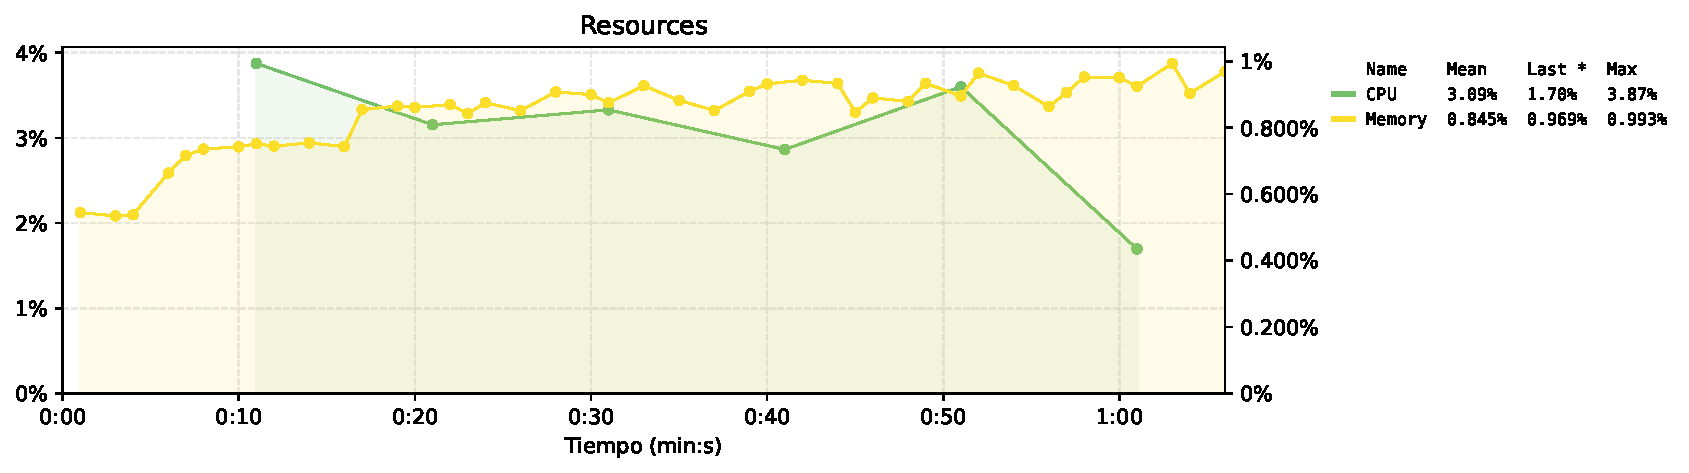
\includegraphics[width=0.8\columnwidth]{figures/sistema_base/race/resources}
            \caption{
                Estado de los recursos del sistema base.
                El eje izquierdo muestra el uso de CPU, el eje derecho muestra el uso de memoria.
            }
            \label{fig:resultados_completos_sistema_base_race_resources}
        \end{figure}

        \begin{figure}[H]
            \centering
            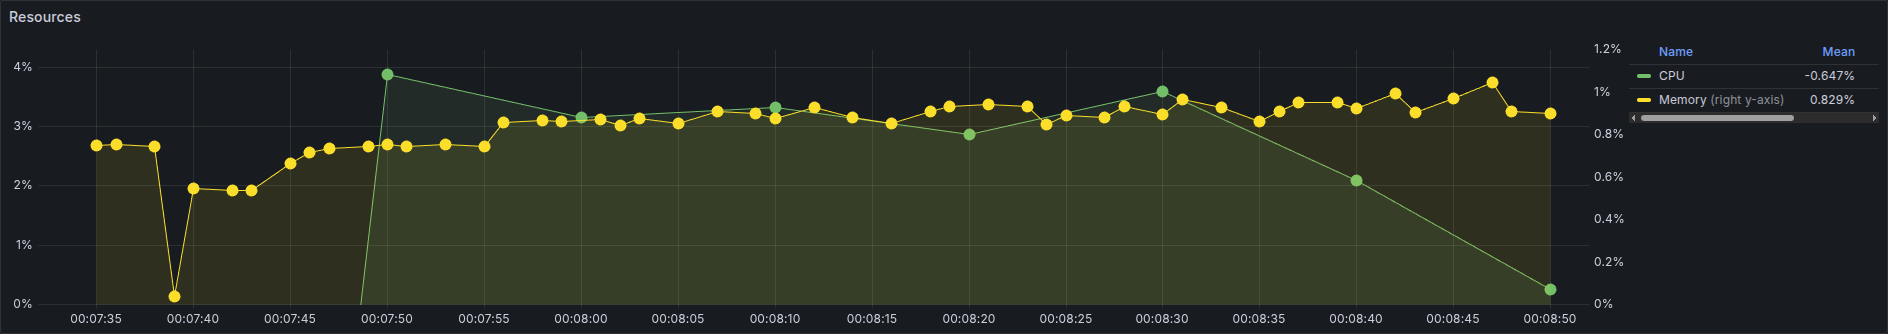
\includegraphics[width=0.8\columnwidth]{figures/sistema_base/race/resources_captura}
            \caption{ Se adjunta la captura correspondiente a la Figura~\ref{fig:resultados_completos_sistema_base_race_resources}. }
            \label{fig:resultados_completos_sistema_base_race_resources_captura}
        \end{figure}

        \begin{figure}[H]
            \centering
            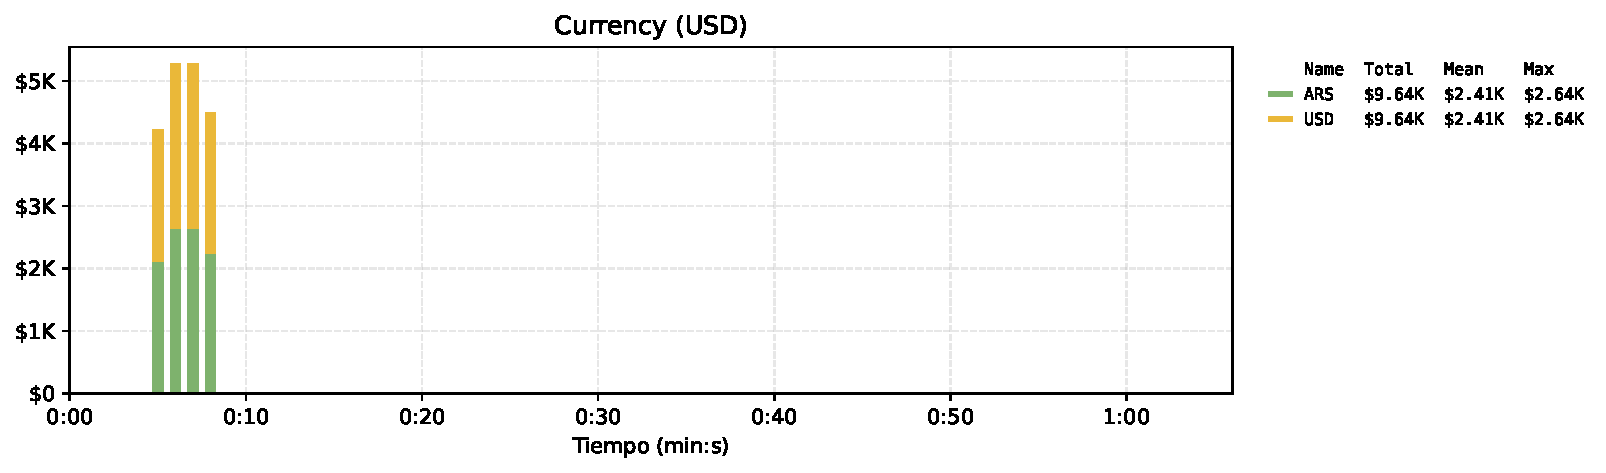
\includegraphics[width=0.8\columnwidth]{figures/sistema_base/race/currency}
            \caption{ Volumen operado en cada moneda en el sistema base. }
            \label{fig:resultados_completos_sistema_base_race_currency}
        \end{figure}

        \begin{figure}[H]
            \centering
            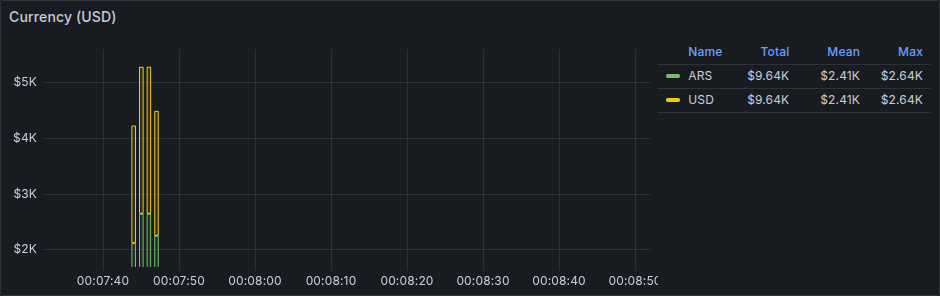
\includegraphics[width=0.8\columnwidth]{figures/sistema_base/race/currency_captura}
            \caption{ Se adjunta la captura correspondiente a la Figura~\ref{fig:resultados_completos_sistema_base_race_currency}. }
            \label{fig:resultados_completos_sistema_base_race_currency_captura}
        \end{figure}

        \begin{figure}[H]
            \centering
            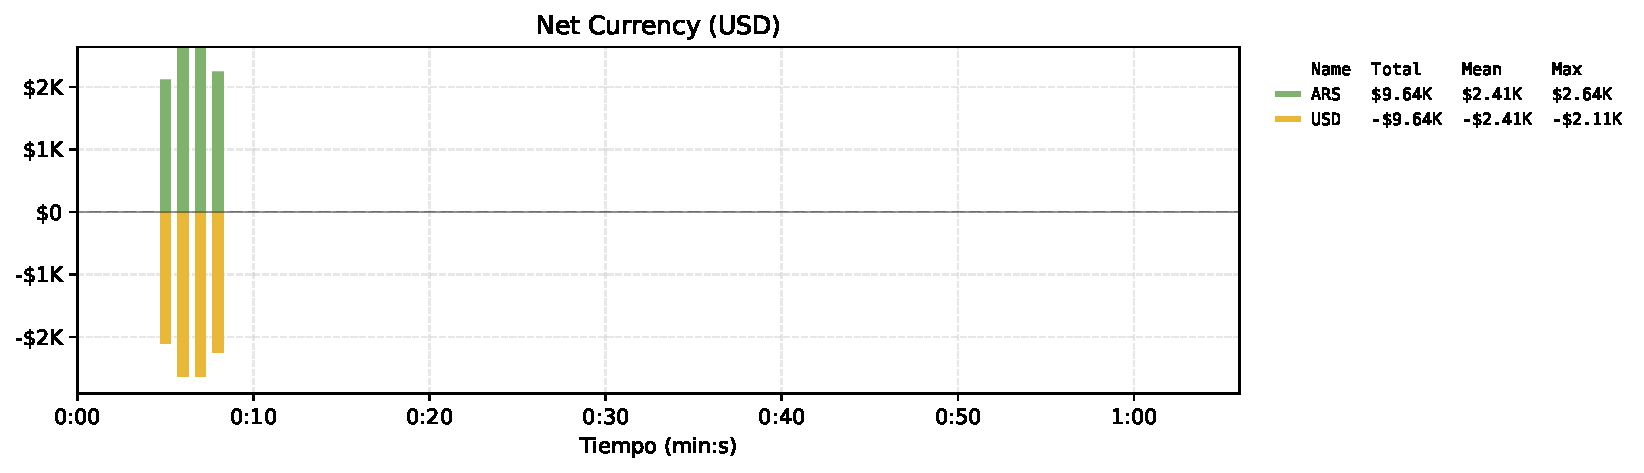
\includegraphics[width=0.8\columnwidth]{figures/sistema_base/race/net_currency}
            \caption{ Neto operado en cada moneda en el sistema base. }
            \label{fig:resultados_completos_sistema_base_race_net_currency}
        \end{figure}

        \begin{figure}[H]
            \centering
            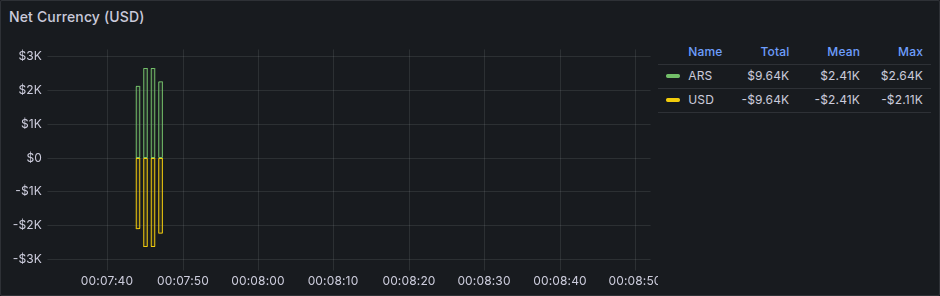
\includegraphics[width=0.8\columnwidth]{figures/sistema_base/race/net_currency_captura}
            \caption{ Se adjunta la captura correspondiente a la Figura~\ref{fig:resultados_completos_sistema_base_race_net_currency}. }
            \label{fig:resultados_completos_sistema_base_race_net_currency_captura}
        \end{figure}

    \clearpage

    \subsection{Resultados completos del escenario de carga sobre la propuesta 1}
    \label{sec:resultados_completos_propuesta_1_baseline}

        \begin{figure}[H]
            \centering
            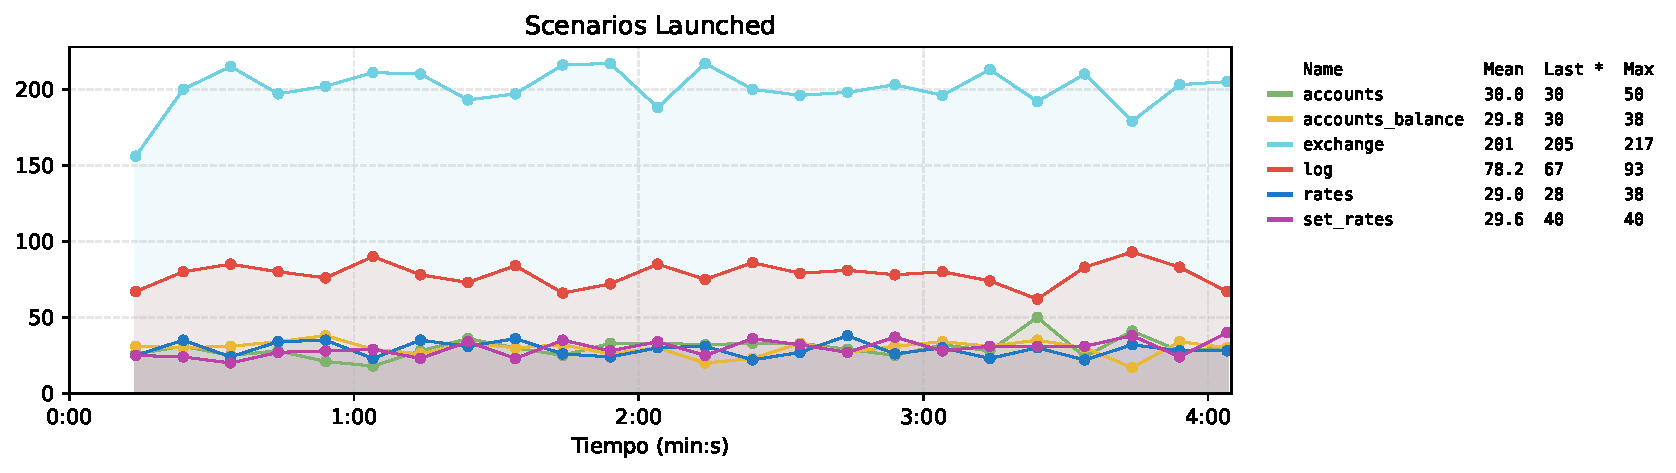
\includegraphics[width=0.8\columnwidth]{figures/propuesta_1/baseline/scenarios}
            \caption{ Escenarios de la propuesta 1. }
            \label{fig:resultados_completos_propuesta_1_baseline_scenarios}
        \end{figure}

        \begin{figure}[H]
            \centering
            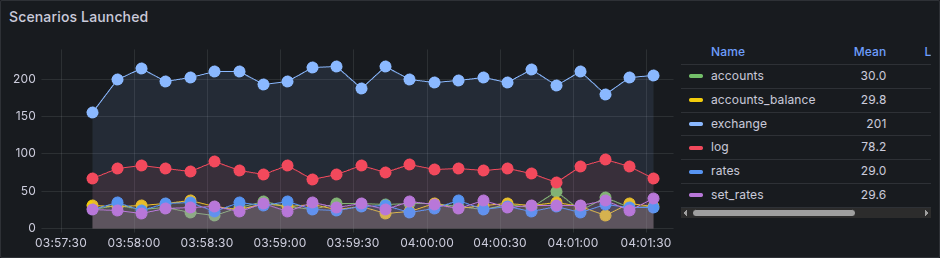
\includegraphics[width=0.8\columnwidth]{figures/propuesta_1/baseline/scenarios_captura}
            \caption{ Se adjunta la captura correspondiente a la Figura~\ref{fig:resultados_completos_propuesta_1_baseline_scenarios}. }
            \label{fig:resultados_completos_propuesta_1_baseline_scenarios_captura}
        \end{figure}

        \begin{figure}[H]
            \centering
            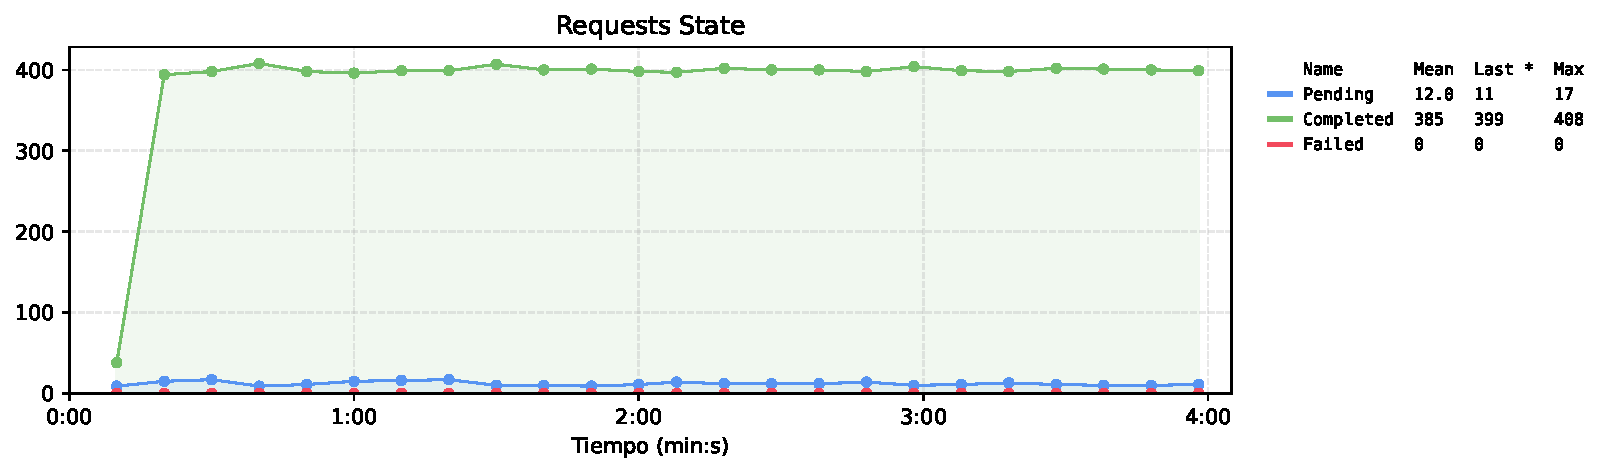
\includegraphics[width=0.8\columnwidth]{figures/propuesta_1/baseline/requests_state}
            \caption{ Estado de las requests de la propuesta 1. }
            \label{fig:resultados_completos_propuesta_1_baseline_requests_state}
        \end{figure}

        \begin{figure}[H]
            \centering
            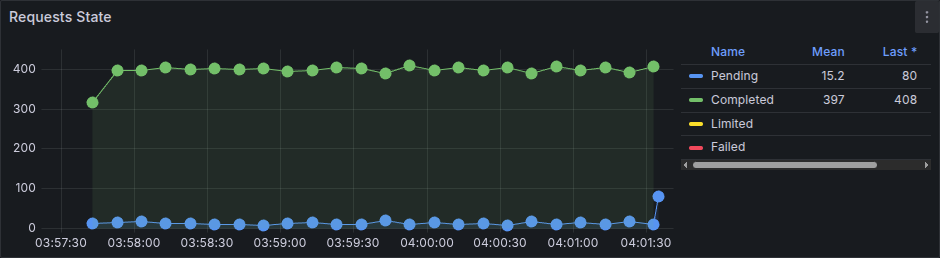
\includegraphics[width=0.8\columnwidth]{figures/propuesta_1/baseline/requests_state_captura}
            \caption{ Se adjunta la captura correspondiente a la Figura~\ref{fig:resultados_completos_propuesta_1_baseline_requests_state}. }
            \label{fig:resultados_completos_propuesta_1_baseline_requests_state_captura}
        \end{figure}

        \begin{figure}[H]
            \centering
            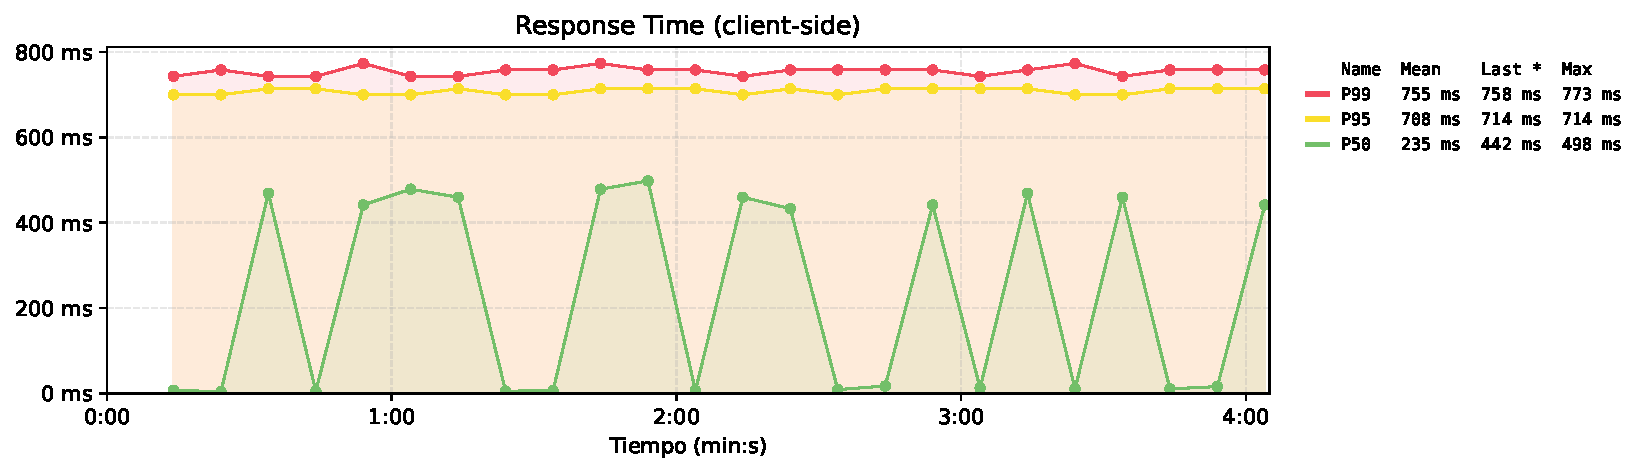
\includegraphics[width=0.8\columnwidth]{figures/propuesta_1/baseline/response_time}
            \caption{ Tiempo de respuesta de la propuesta 1. }
            \label{fig:resultados_completos_propuesta_1_baseline_response_time}
        \end{figure}

        \begin{figure}[H]
            \centering
            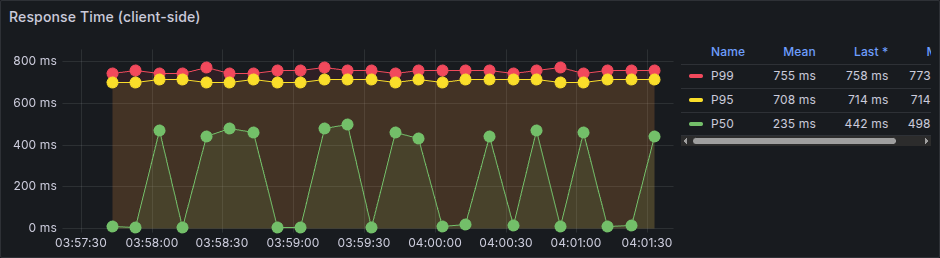
\includegraphics[width=0.8\columnwidth]{figures/propuesta_1/baseline/response_time_captura}
            \caption{ Se adjunta la captura correspondiente a la Figura~\ref{fig:resultados_completos_propuesta_1_baseline_response_time}. }
            \label{fig:resultados_completos_propuesta_1_baseline_response_time_captura}
        \end{figure}

        \begin{figure}[H]
            \centering
            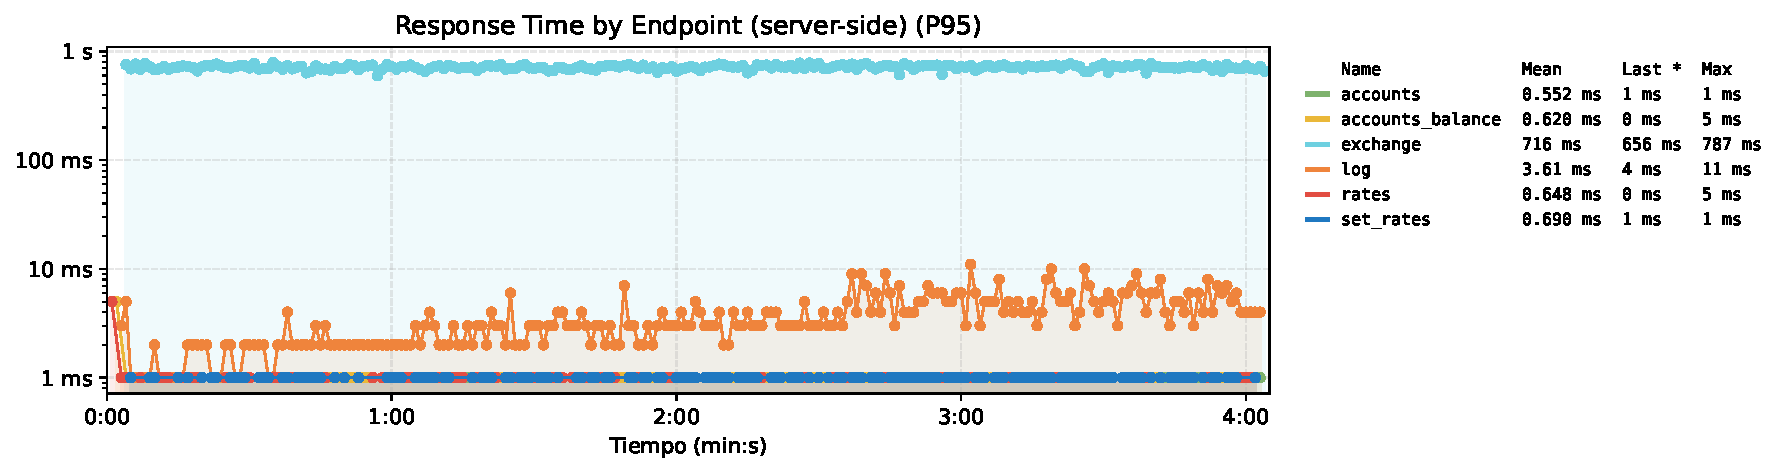
\includegraphics[width=0.8\columnwidth]{figures/propuesta_1/baseline/endpoint_response_time}
            \caption{
                Tiempo de respuesta por endpoint de la propuesta 1.
                El eje tiene una escala logarítmica.
            }
            \label{fig:resultados_completos_propuesta_1_baseline_endpoint_response_time}
        \end{figure}

        \begin{figure}[H]
            \centering
            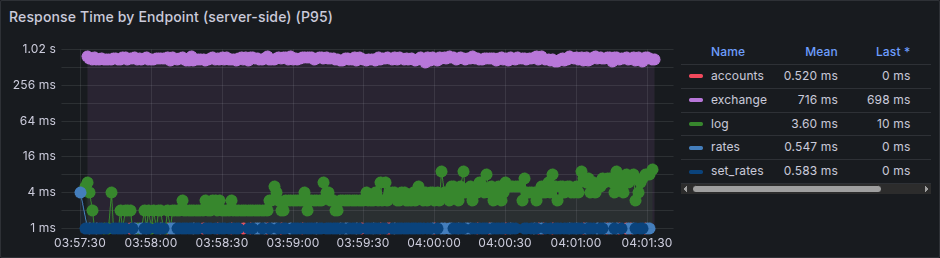
\includegraphics[width=0.8\columnwidth]{figures/propuesta_1/baseline/endpoint_response_time_captura}
            \caption{ Se adjunta la captura correspondiente a la Figura~\ref{fig:resultados_completos_propuesta_1_baseline_endpoint_response_time}. }
            \label{fig:resultados_completos_propuesta_1_baseline_endpoint_response_time_captura}
        \end{figure}

        \begin{figure}[H]
            \centering
            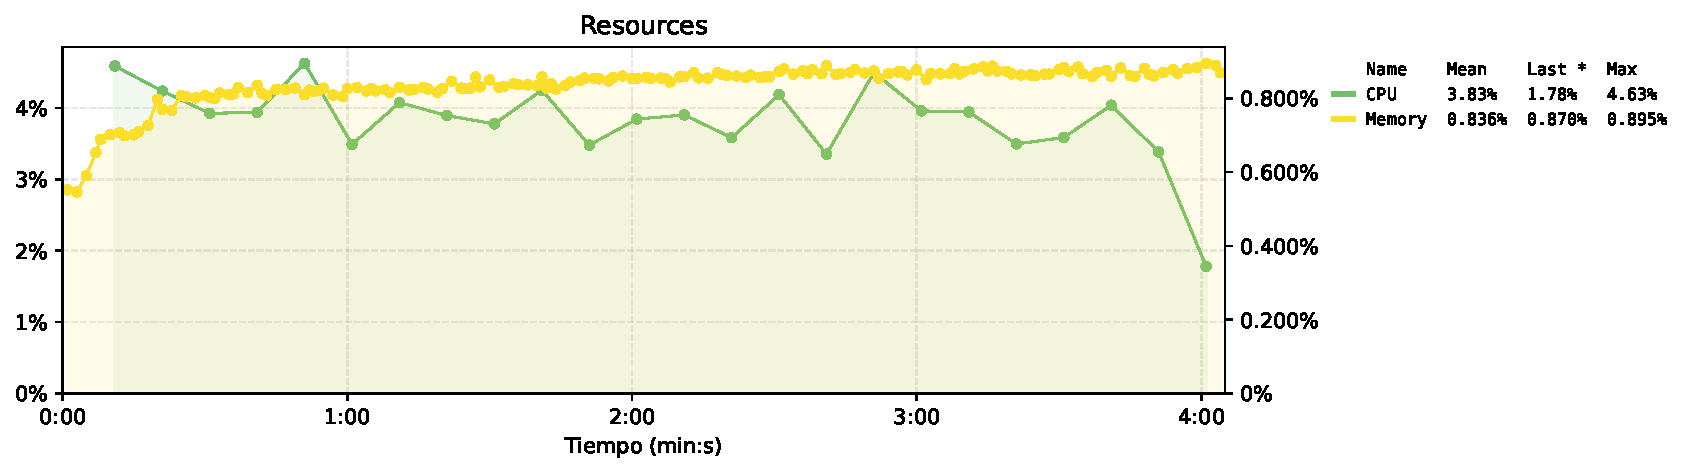
\includegraphics[width=0.8\columnwidth]{figures/propuesta_1/baseline/resources}
            \caption{
                Estado de los recursos del nodo de exchange de la propuesta 1.
                El eje izquierdo muestra el uso de CPU, el eje derecho muestra el uso de memoria.
            }
            \label{fig:resultados_completos_propuesta_1_baseline_resources}
        \end{figure}

        \begin{figure}[H]
            \centering
            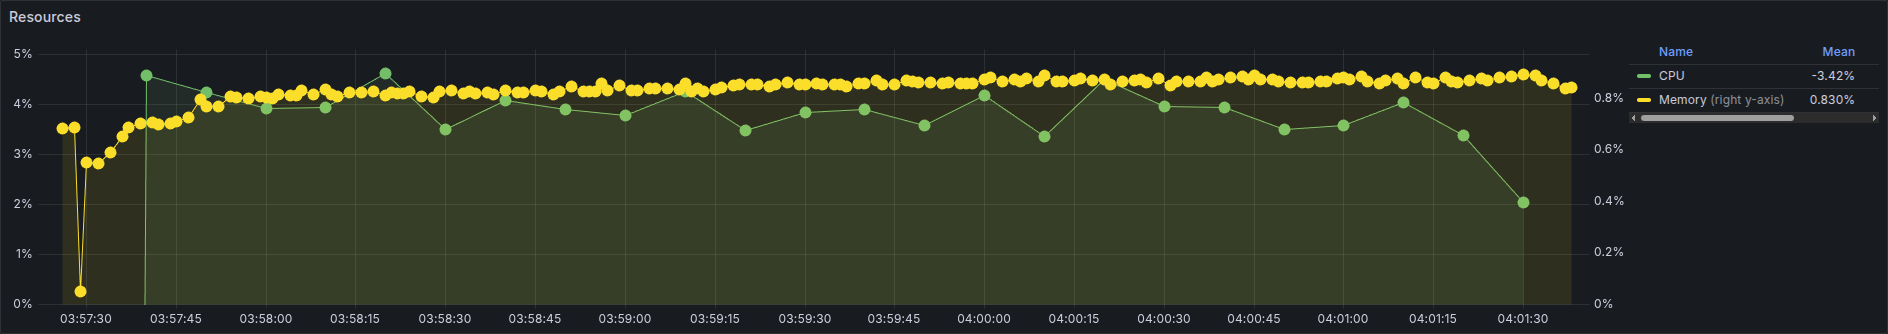
\includegraphics[width=0.8\columnwidth]{figures/propuesta_1/baseline/resources_captura}
            \caption{ Se adjunta la captura correspondiente a la Figura~\ref{fig:resultados_completos_propuesta_1_baseline_resources}. }
            \label{fig:resultados_completos_propuesta_1_baseline_resources_captura}
        \end{figure}

        \begin{figure}[H]
            \centering
            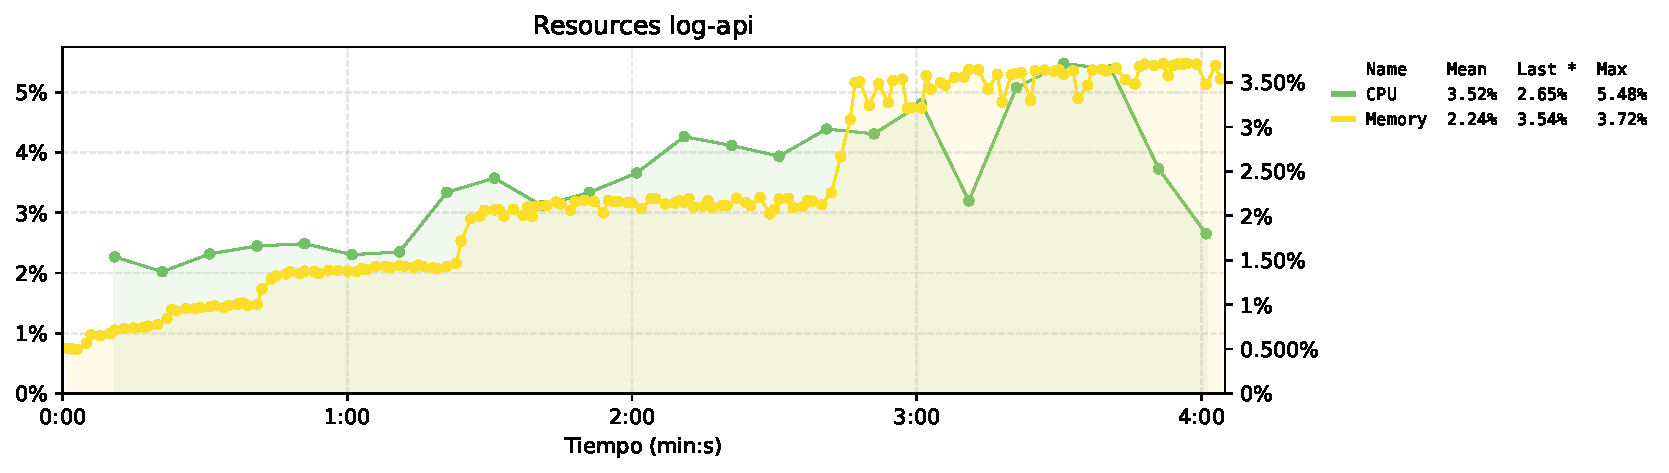
\includegraphics[width=0.8\columnwidth]{figures/propuesta_1/baseline/resources_log_api}
            \caption{
                Estado de los recursos del nodo de logs de la propuesta 1.
                El eje izquierdo muestra el uso de CPU, el eje derecho muestra el uso de memoria.
            }
            \label{fig:resultados_completos_propuesta_1_baseline_resources_log_api}
        \end{figure}

        \begin{figure}[H]
            \centering
            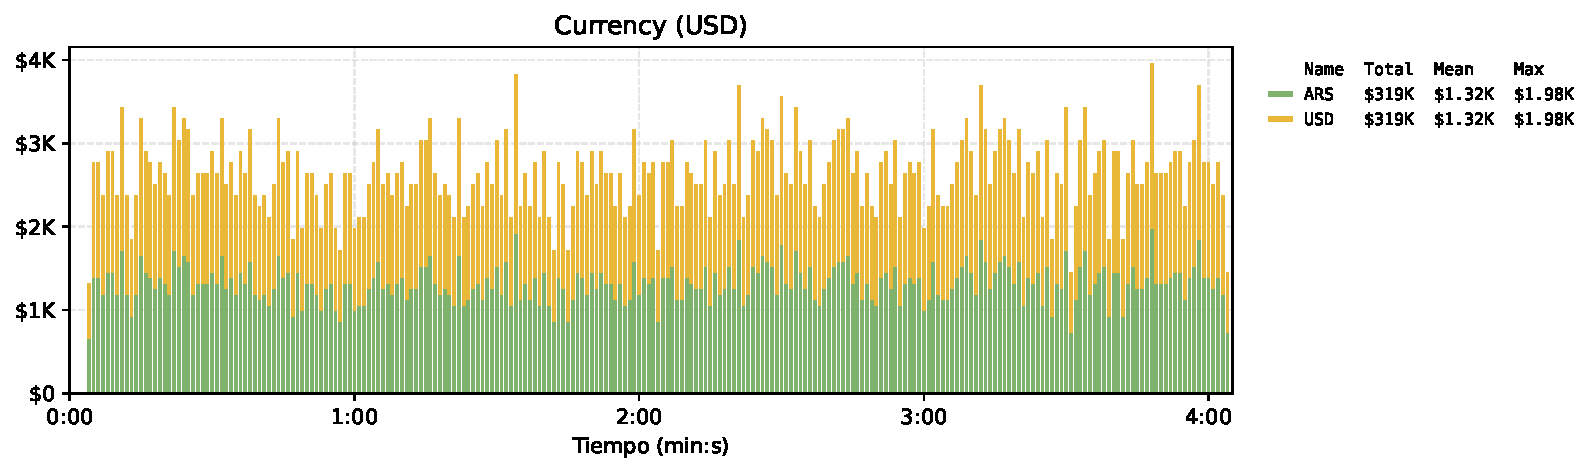
\includegraphics[width=0.8\columnwidth]{figures/propuesta_1/baseline/currency}
            \caption{ Volumen operado en cada moneda en la propuesta 1. }
            \label{fig:resultados_completos_propuesta_1_baseline_currency}
        \end{figure}

        \begin{figure}[H]
            \centering
            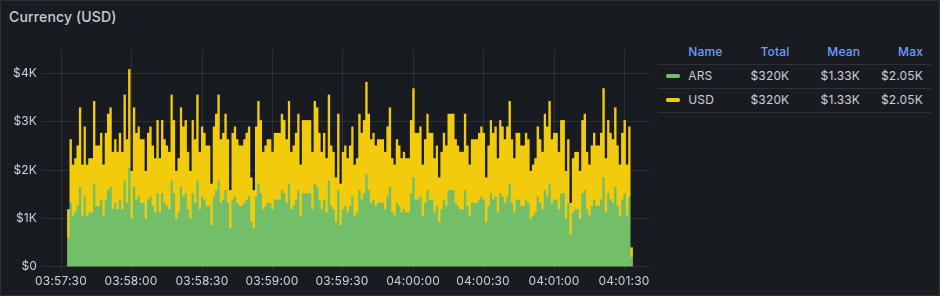
\includegraphics[width=0.8\columnwidth]{figures/propuesta_1/baseline/currency_captura}
            \caption{ Se adjunta la captura correspondiente a la Figura~\ref{fig:resultados_completos_propuesta_1_baseline_currency}. }
            \label{fig:resultados_completos_propuesta_1_baseline_currency_captura}
        \end{figure}

        \begin{figure}[H]
            \centering
            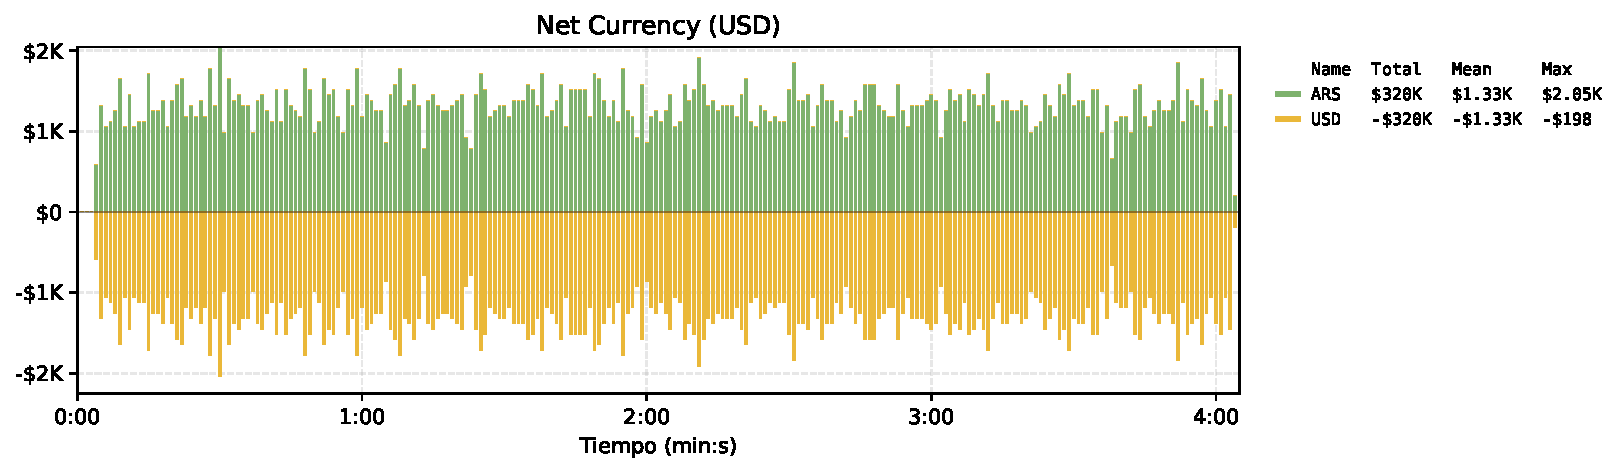
\includegraphics[width=0.8\columnwidth]{figures/propuesta_1/baseline/net_currency}
            \caption{ Neto operado en cada moneda en la propuesta 1. }
            \label{fig:resultados_completos_propuesta_1_baseline_net_currency}
        \end{figure}

        \begin{figure}[H]
            \centering
            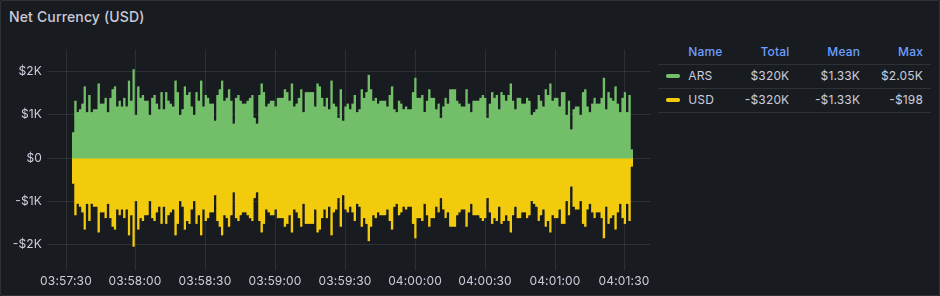
\includegraphics[width=0.8\columnwidth]{figures/propuesta_1/baseline/net_currency_captura}
            \caption{ Se adjunta la captura correspondiente a la Figura~\ref{fig:resultados_completos_propuesta_1_baseline_net_currency}. }
            \label{fig:resultados_completos_propuesta_1_baseline_net_currency_captura}
        \end{figure}

    \clearpage

    \subsection{Resultados completos del escenario de estrés sobre la propuesta 1}
    \label{sec:resultados_completos_propuesta_1_stress}

        \begin{figure}[H]
            \centering
            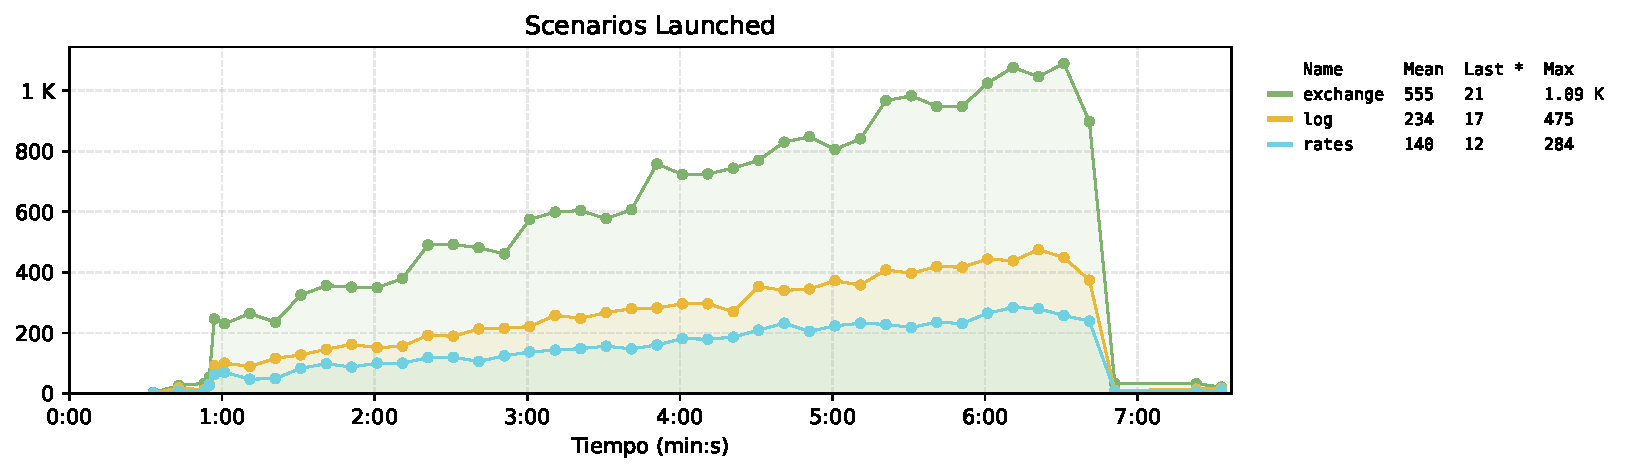
\includegraphics[width=0.8\columnwidth]{figures/propuesta_1/stress/scenarios}
            \caption{ Escenarios de la propuesta 1. }
            \label{fig:resultados_completos_propuesta_1_stress_scenarios}
        \end{figure}

        \begin{figure}[H]
            \centering
            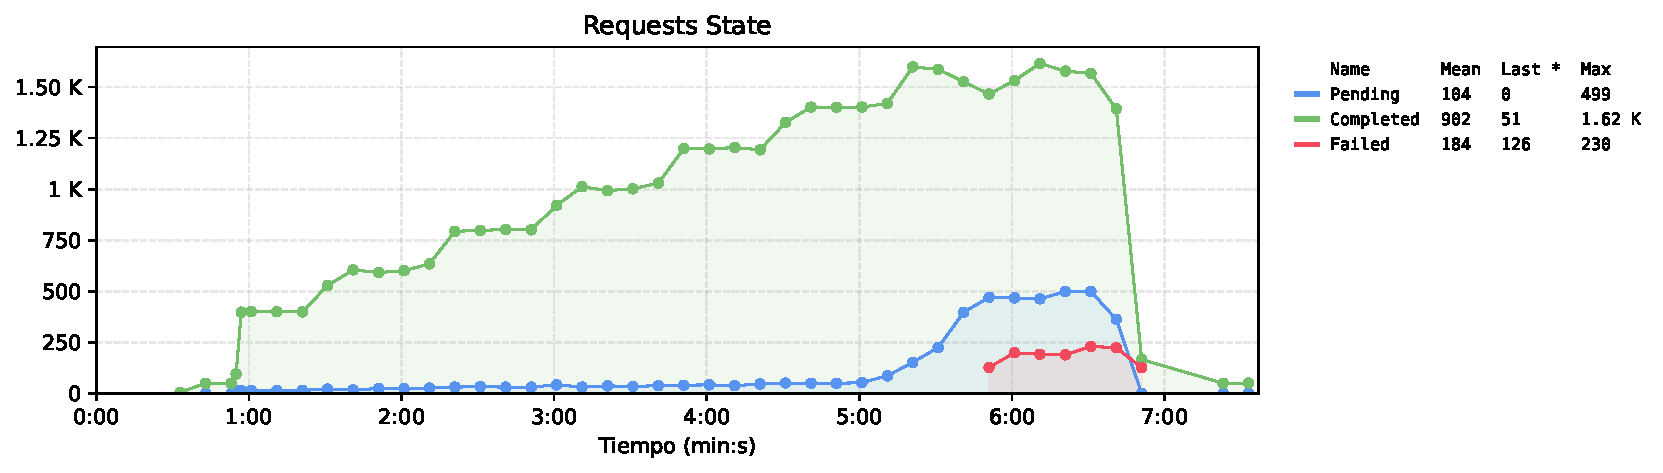
\includegraphics[width=0.8\columnwidth]{figures/propuesta_1/stress/requests_state}
            \caption{ Estado de las requests de la propuesta 1. }
            \label{fig:resultados_completos_propuesta_1_stress_requests_state}
        \end{figure}

        \begin{figure}[H]
            \centering
            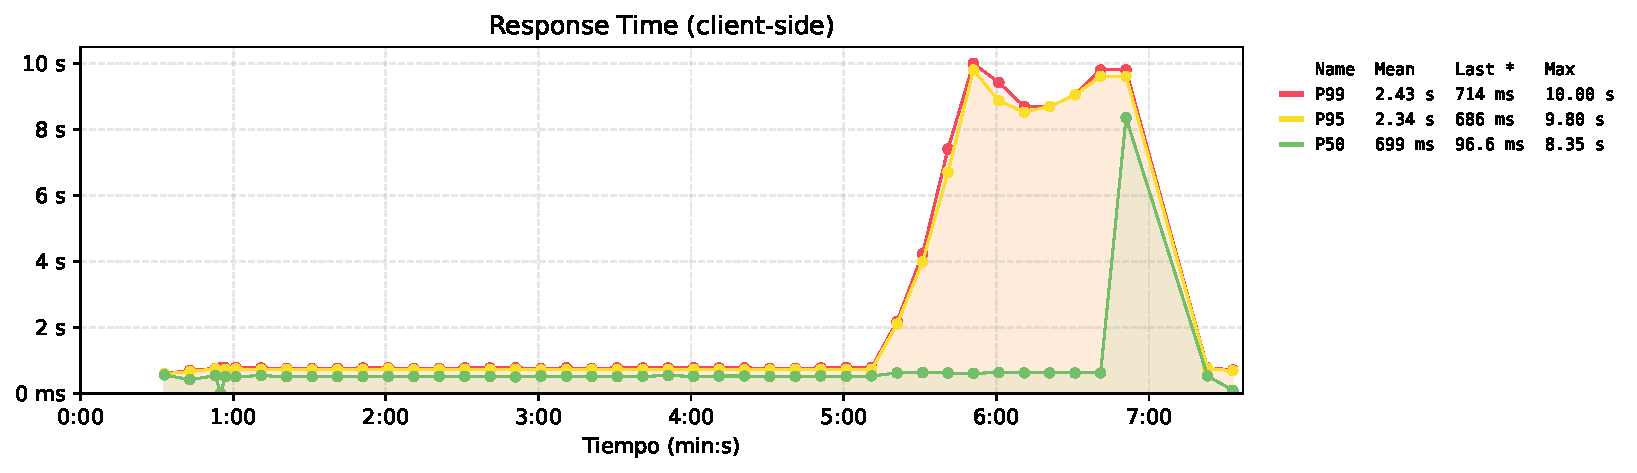
\includegraphics[width=0.8\columnwidth]{figures/propuesta_1/stress/response_time}
            \caption{ Tiempo de respuesta de la propuesta 1. }
            \label{fig:resultados_completos_propuesta_1_stress_response_time}
        \end{figure}

        \begin{figure}[H]
            \centering
            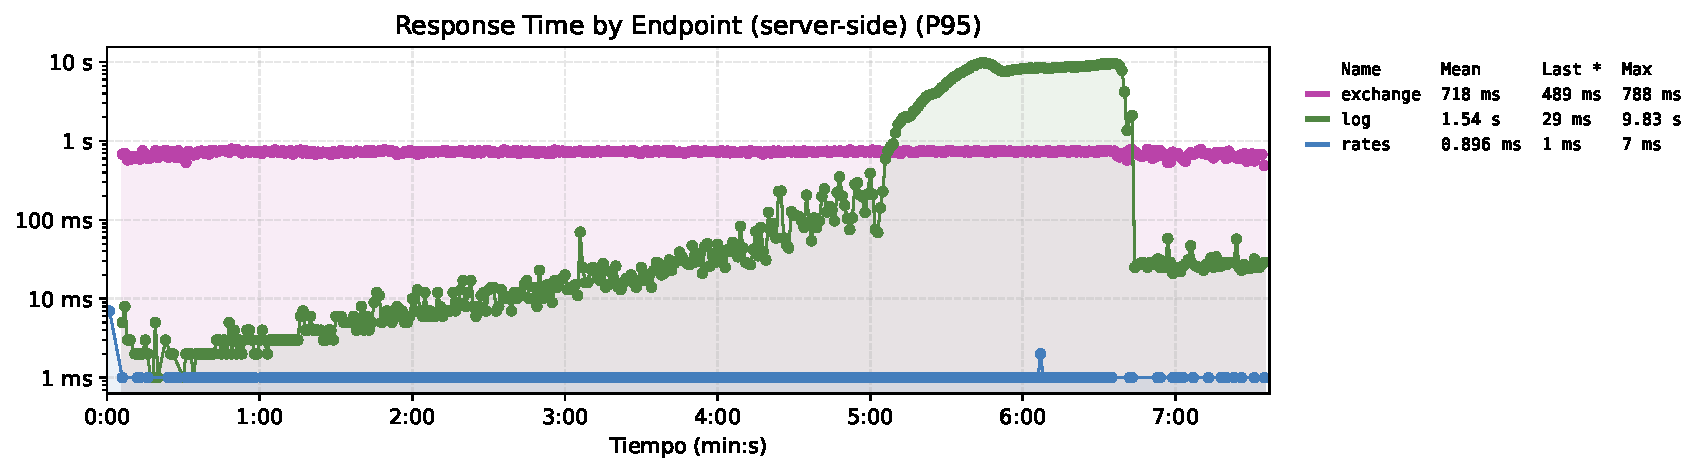
\includegraphics[width=0.8\columnwidth]{figures/propuesta_1/stress/endpoint_response_time}
            \caption{
                Tiempo de respuesta por endpoint de la propuesta 1.
                El eje tiene una escala logarítmica.
            }
            \label{fig:resultados_completos_propuesta_1_stress_endpoint_response_time}
        \end{figure}

        \begin{figure}[H]
            \centering
            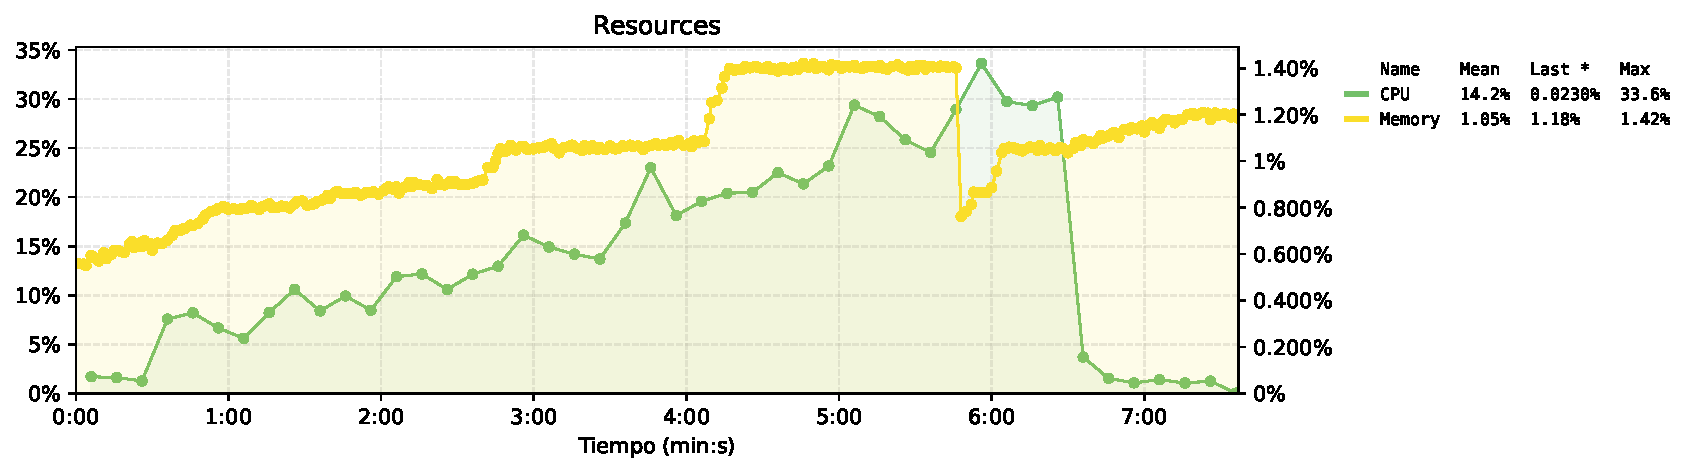
\includegraphics[width=0.8\columnwidth]{figures/propuesta_1/stress/resources}
            \caption{
                Estado de los recursos del nodo de exchange de la propuesta 1.
                El eje izquierdo muestra el uso de CPU, el eje derecho muestra el uso de memoria.
            }
            \label{fig:resultados_completos_propuesta_1_stress_resources}
        \end{figure}

        \begin{figure}[H]
            \centering
            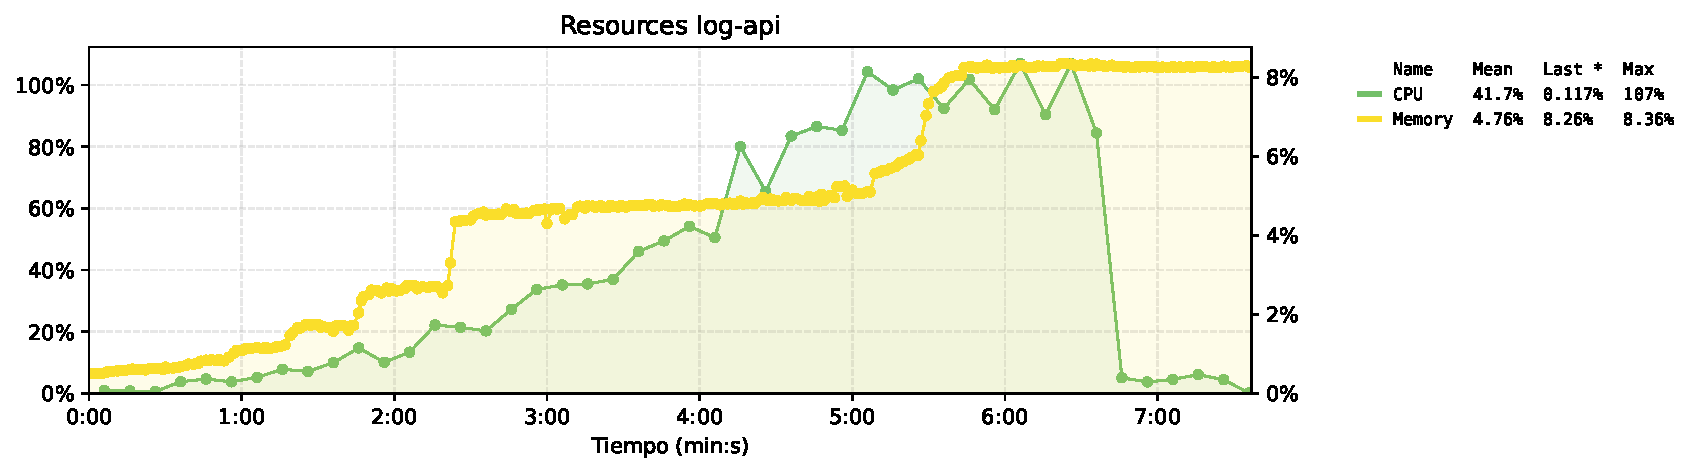
\includegraphics[width=0.8\columnwidth]{figures/propuesta_1/stress/resources_log_api}
            \caption{
                Estado de los recursos del nodo de logs de la propuesta 1.
                El eje izquierdo muestra el uso de CPU, el eje derecho muestra el uso de memoria.
            }
            \label{fig:resultados_completos_propuesta_1_stress_resources_log_api}
        \end{figure}

        \begin{figure}[H]
            \centering
            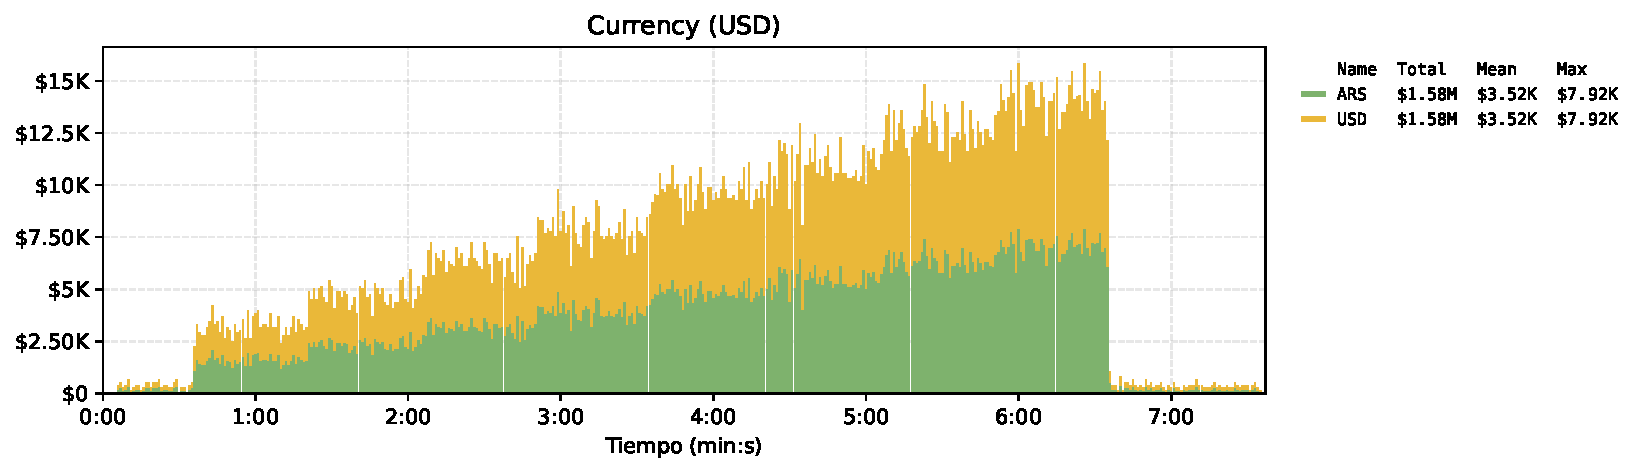
\includegraphics[width=0.8\columnwidth]{figures/propuesta_1/stress/currency}
            \caption{ Volumen operado en cada moneda en la propuesta 1. }
            \label{fig:resultados_completos_propuesta_1_stress_currency}
        \end{figure}

        \begin{figure}[H]
            \centering
            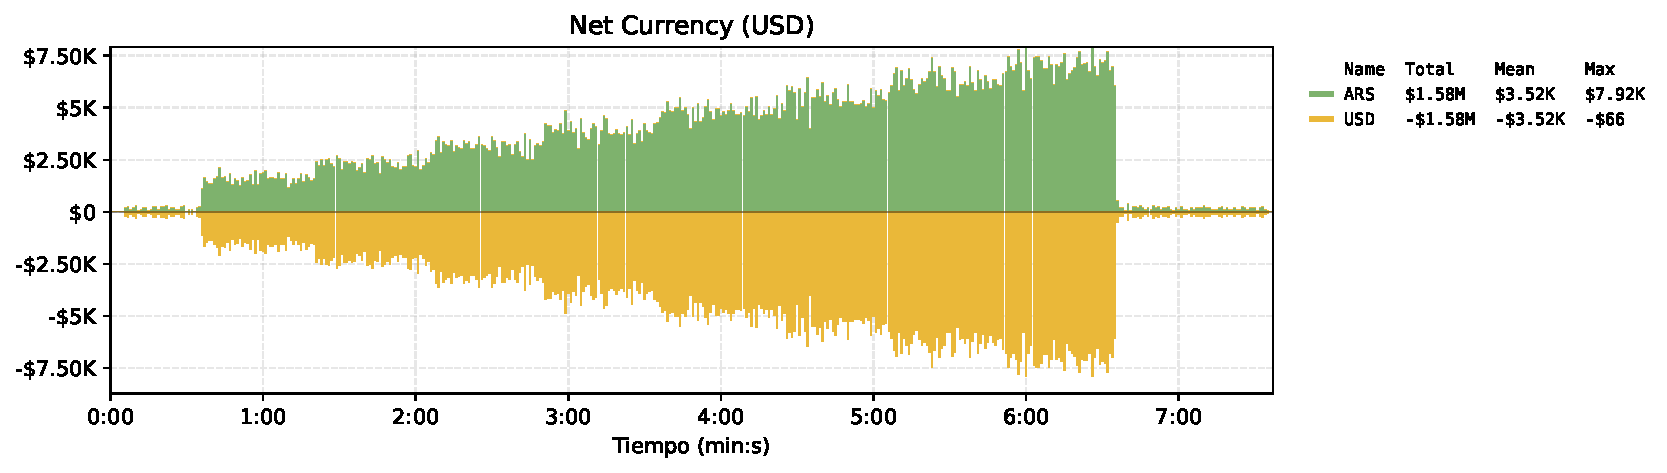
\includegraphics[width=0.8\columnwidth]{figures/propuesta_1/stress/net_currency}
            \caption{ Neto operado en cada moneda en la propuesta 1. }
            \label{fig:resultados_completos_propuesta_1_stress_net_currency}
        \end{figure}

    \clearpage

    \subsection{Resultados completos del escenario de resistencia sobre la propuesta 1}
    \label{sec:resultados_completos_propuesta_1_soak}

        \begin{figure}[H]
            \centering
            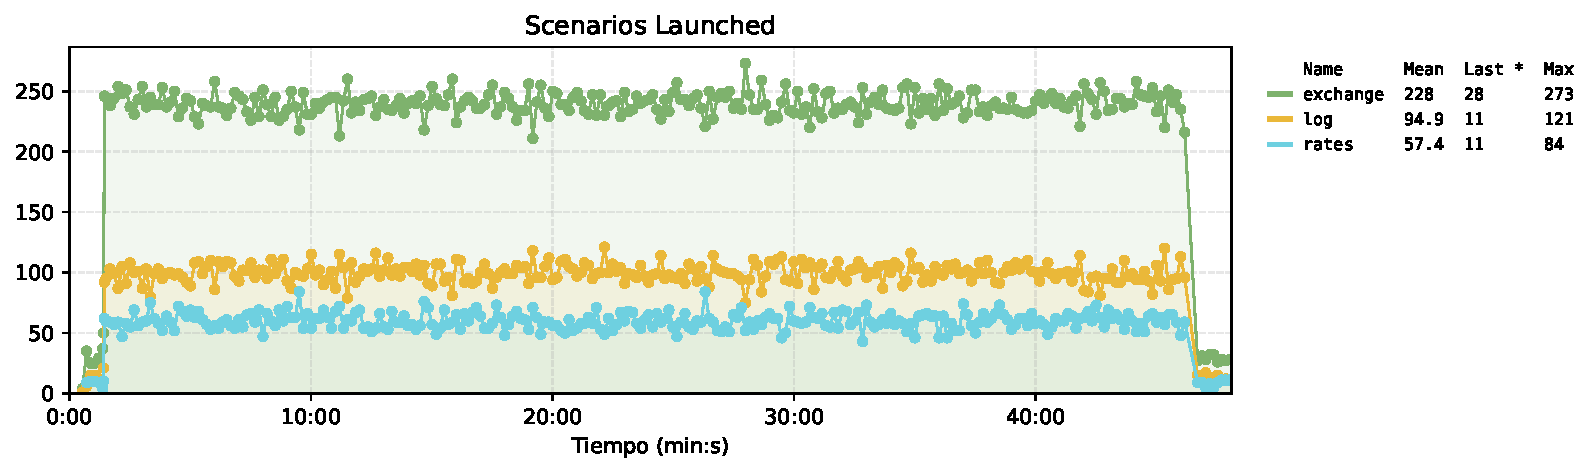
\includegraphics[width=0.8\columnwidth]{figures/propuesta_1/soak/scenarios}
            \caption{ Escenarios de la propuesta 1. }
            \label{fig:resultados_completos_propuesta_1_soak_scenarios}
        \end{figure}

        \begin{figure}[H]
            \centering
            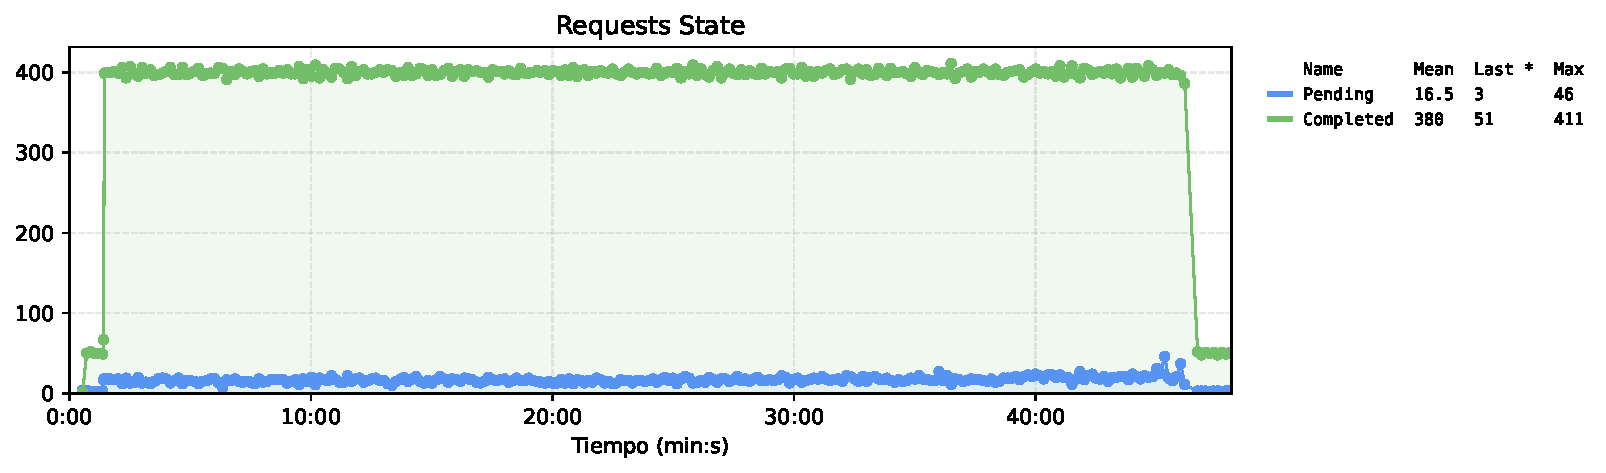
\includegraphics[width=0.8\columnwidth]{figures/propuesta_1/soak/requests_state}
            \caption{ Estado de las requests de la propuesta 1. }
            \label{fig:resultados_completos_propuesta_1_soak_requests_state}
        \end{figure}

        \begin{figure}[H]
            \centering
            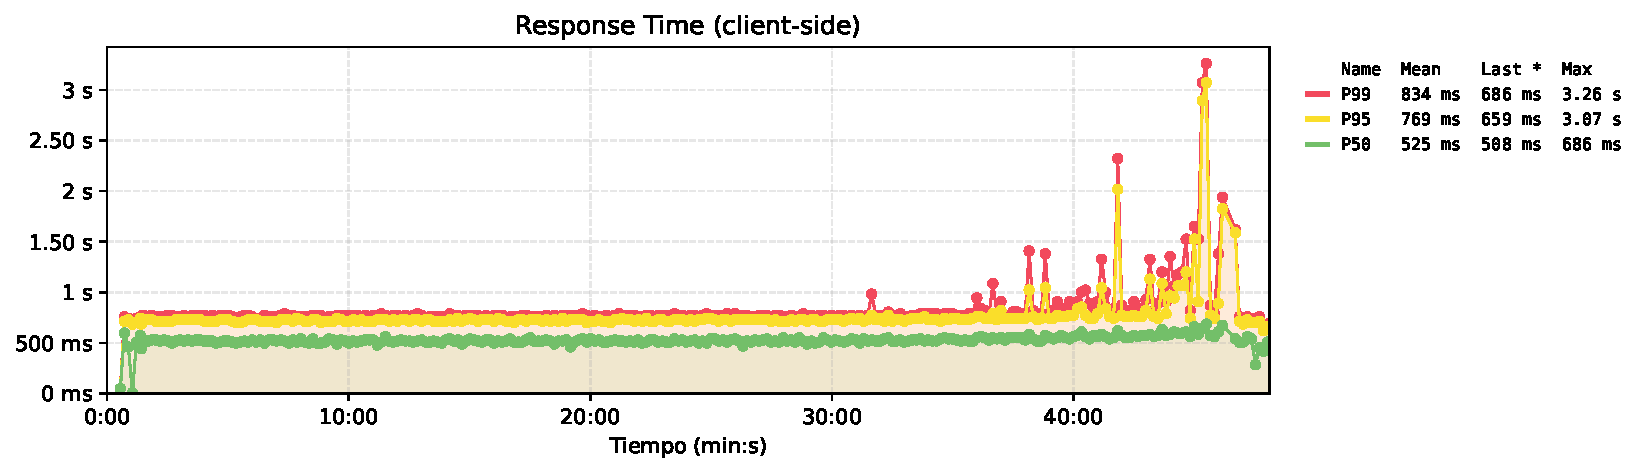
\includegraphics[width=0.8\columnwidth]{figures/propuesta_1/soak/response_time}
            \caption{ Tiempo de respuesta de la propuesta 1. }
            \label{fig:resultados_completos_propuesta_1_soak_response_time}
        \end{figure}

        \begin{figure}[H]
            \centering
            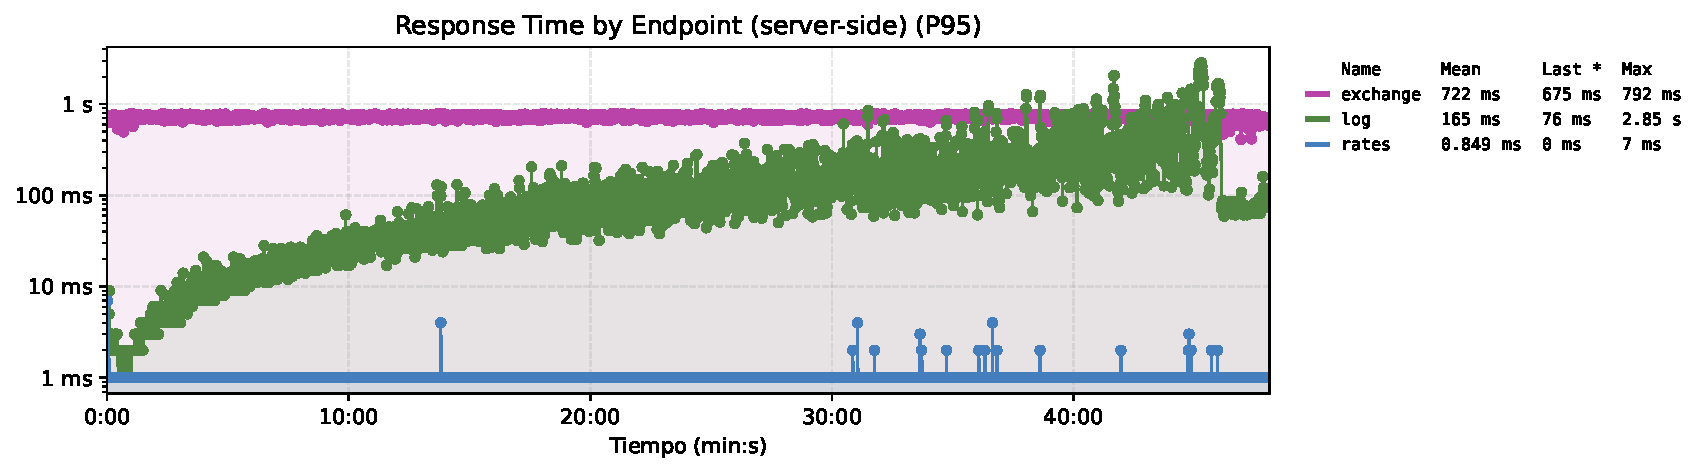
\includegraphics[width=0.8\columnwidth]{figures/propuesta_1/soak/endpoint_response_time}
            \caption{
                Tiempo de respuesta por endpoint de la propuesta 1.
                El eje tiene una escala logarítmica.
            }
            \label{fig:resultados_completos_propuesta_1_soak_endpoint_response_time}
        \end{figure}

        \begin{figure}[H]
            \centering
            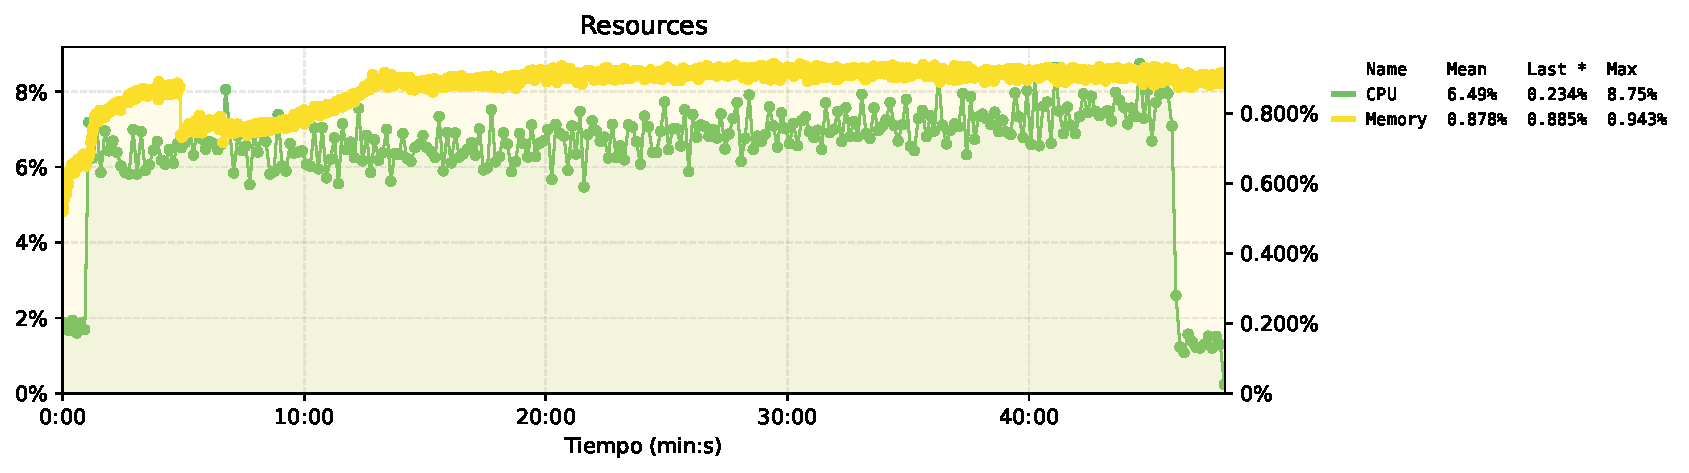
\includegraphics[width=0.8\columnwidth]{figures/propuesta_1/soak/resources}
            \caption{
                Estado de los recursos del nodo de exchange de la propuesta 1.
                El eje izquierdo muestra el uso de CPU, el eje derecho muestra el uso de memoria.
            }
            \label{fig:resultados_completos_propuesta_1_soak_resources}
        \end{figure}

        \begin{figure}[H]
            \centering
            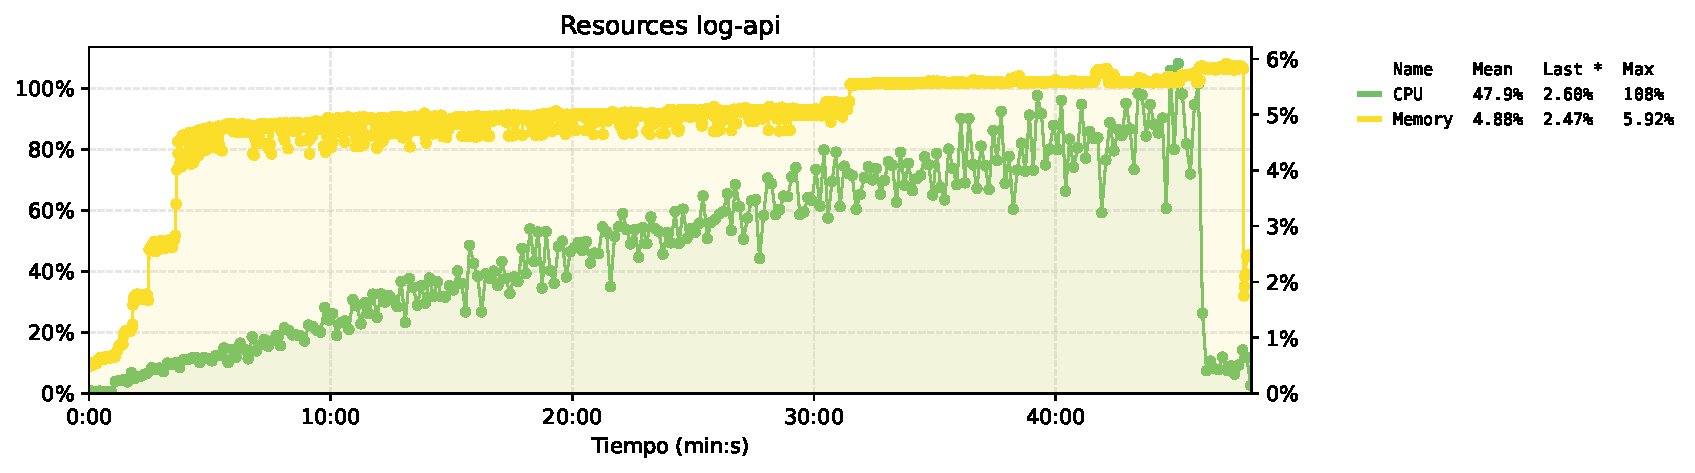
\includegraphics[width=0.8\columnwidth]{figures/propuesta_1/soak/resources_log_api}
            \caption{
                Estado de los recursos del nodo de logs de la propuesta 1.
                El eje izquierdo muestra el uso de CPU, el eje derecho muestra el uso de memoria.
            }
            \label{fig:resultados_completos_propuesta_1_soak_resources_log_api}
        \end{figure}

        \begin{figure}[H]
            \centering
            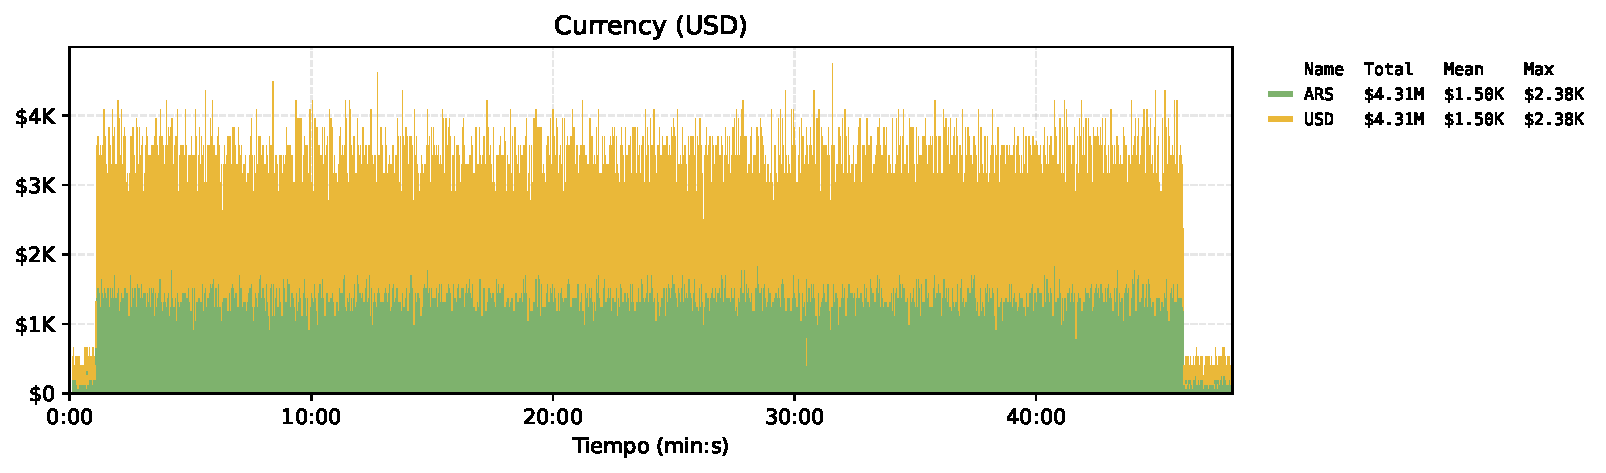
\includegraphics[width=0.8\columnwidth]{figures/propuesta_1/soak/currency}
            \caption{ Volumen operado en cada moneda en la propuesta 1. }
            \label{fig:resultados_completos_propuesta_1_soak_currency}
        \end{figure}

        \begin{figure}[H]
            \centering
            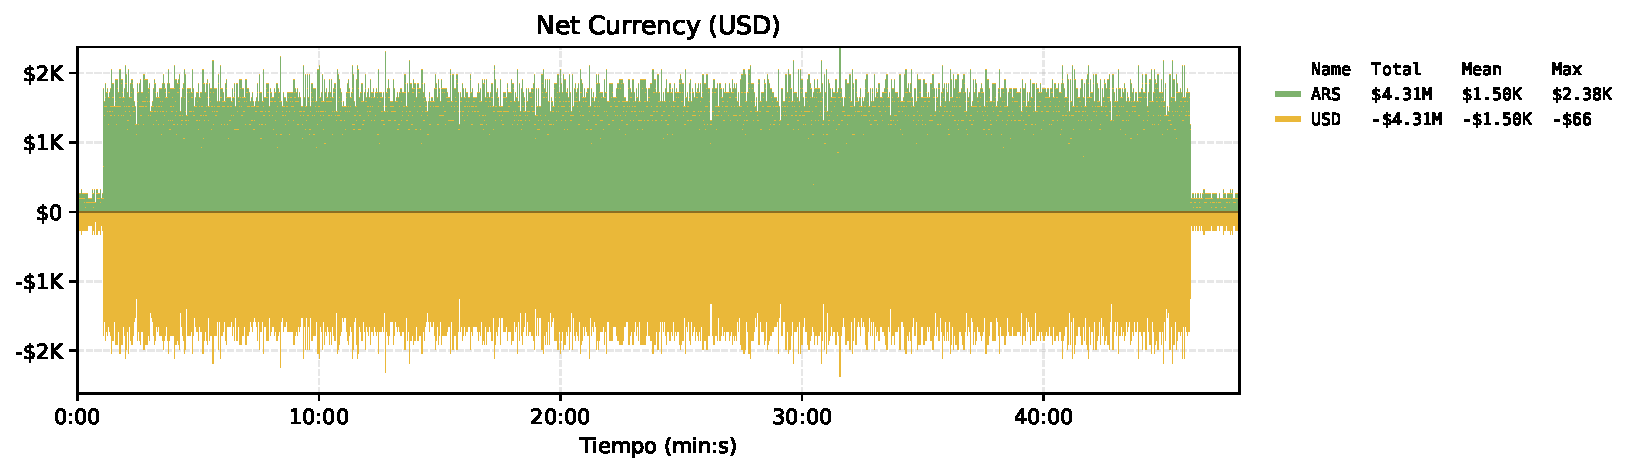
\includegraphics[width=0.8\columnwidth]{figures/propuesta_1/soak/net_currency}
            \caption{ Neto operado en cada moneda en la propuesta 1. }
            \label{fig:resultados_completos_propuesta_1_soak_net_currency}
        \end{figure}

    \clearpage

    \subsection{Resultados completos del escenario de carga sobre la propuesta 2}
    \label{sec:resultados_completos_propuesta_2_baseline}

        \begin{figure}[H]
            \centering
            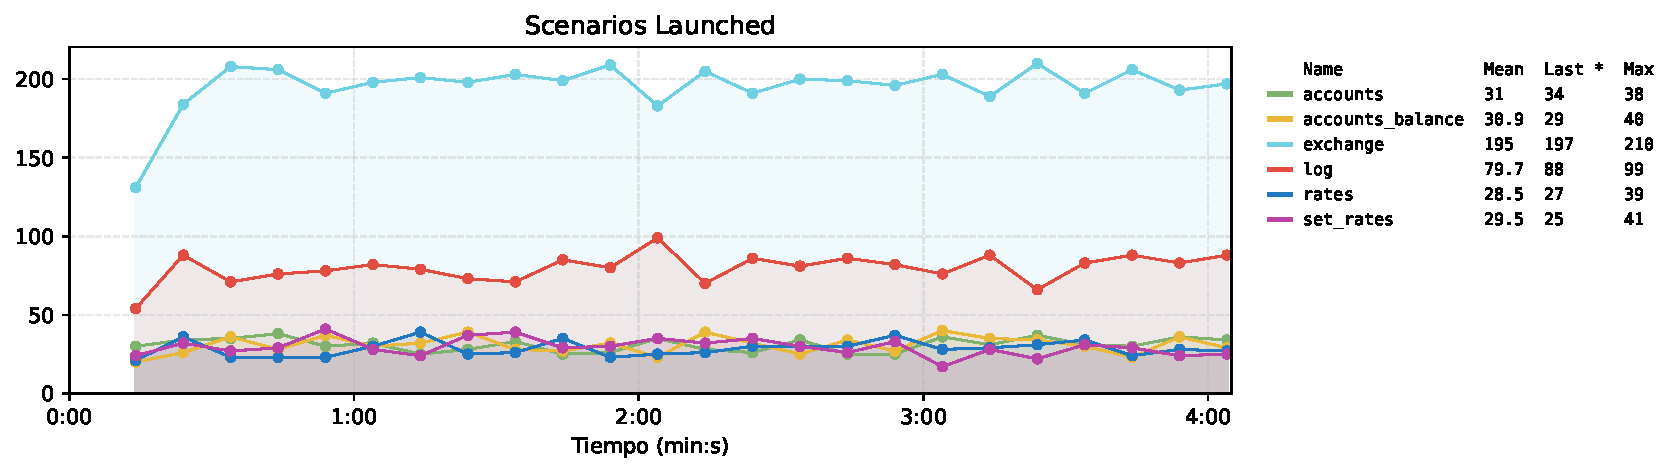
\includegraphics[width=0.8\columnwidth]{figures/propuesta_2/baseline/scenarios}
            \caption{ Escenarios de la propuesta 2. }
            \label{fig:resultados_completos_propuesta_2_baseline_scenarios}
        \end{figure}

        \begin{figure}[H]
            \centering
            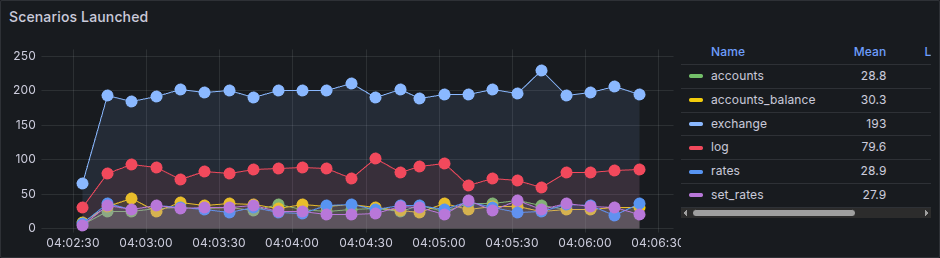
\includegraphics[width=0.8\columnwidth]{figures/propuesta_2/baseline/scenarios_captura}
            \caption{ Se adjunta la captura correspondiente a la Figura~\ref{fig:resultados_completos_propuesta_2_baseline_scenarios}. }
            \label{fig:resultados_completos_propuesta_2_baseline_scenarios_captura}
        \end{figure}

        \begin{figure}[H]
            \centering
            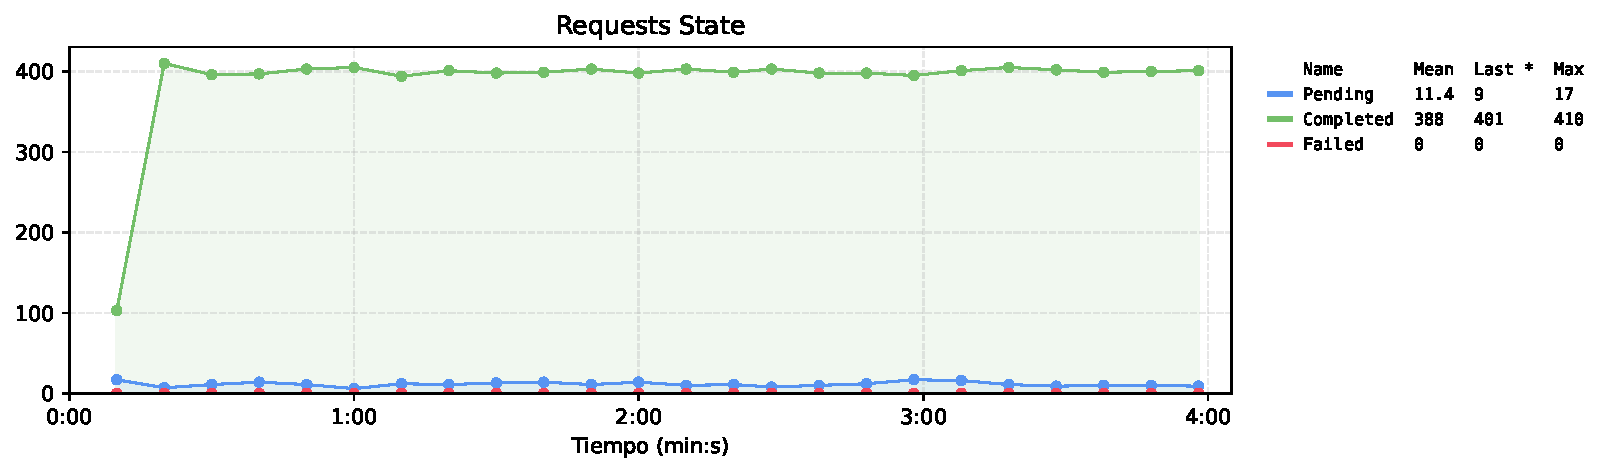
\includegraphics[width=0.8\columnwidth]{figures/propuesta_2/baseline/requests_state}
            \caption{ Estado de las requests de la propuesta 2. }
            \label{fig:resultados_completos_propuesta_2_baseline_requests_state}
        \end{figure}

        \begin{figure}[H]
            \centering
            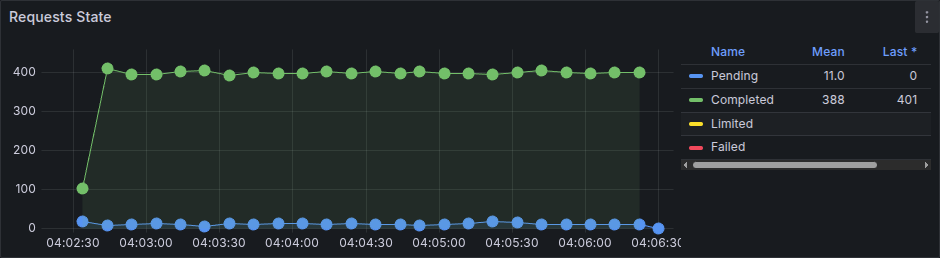
\includegraphics[width=0.8\columnwidth]{figures/propuesta_2/baseline/requests_state_captura}
            \caption{ Se adjunta la captura correspondiente a la Figura~\ref{fig:resultados_completos_propuesta_2_baseline_requests_state}. }
            \label{fig:resultados_completos_propuesta_2_baseline_requests_state_captura}
        \end{figure}

        \begin{figure}[H]
            \centering
            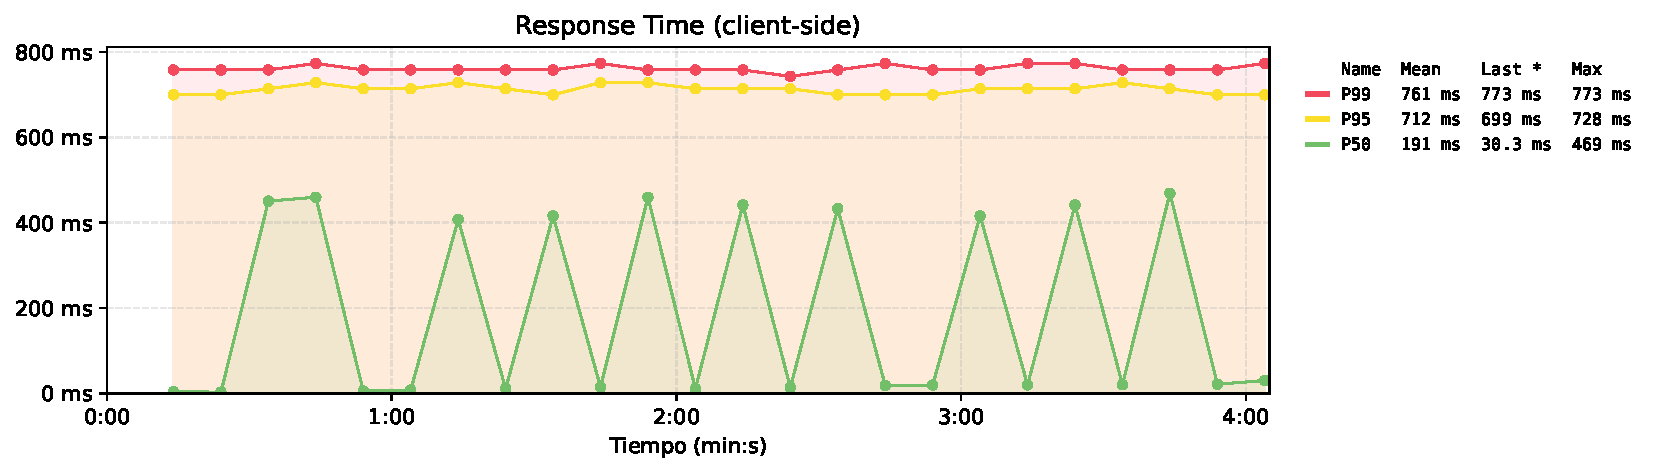
\includegraphics[width=0.8\columnwidth]{figures/propuesta_2/baseline/response_time}
            \caption{ Tiempo de respuesta de la propuesta 2. }
            \label{fig:resultados_completos_propuesta_2_baseline_response_time}
        \end{figure}

        \begin{figure}[H]
            \centering
            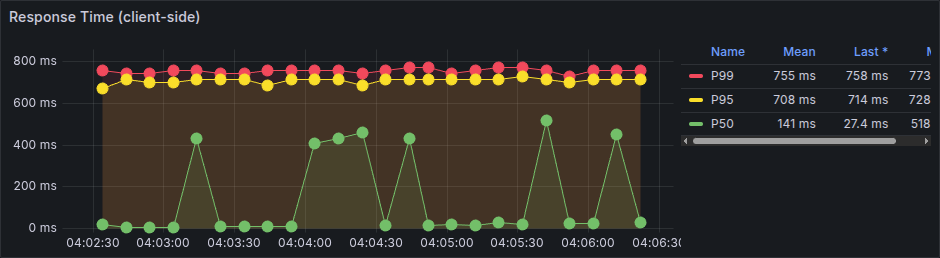
\includegraphics[width=0.8\columnwidth]{figures/propuesta_2/baseline/response_time_captura}
            \caption{ Se adjunta la captura correspondiente a la Figura~\ref{fig:resultados_completos_propuesta_2_baseline_response_time}. }
            \label{fig:resultados_completos_propuesta_2_baseline_response_time_captura}
        \end{figure}

        \begin{figure}[H]
            \centering
            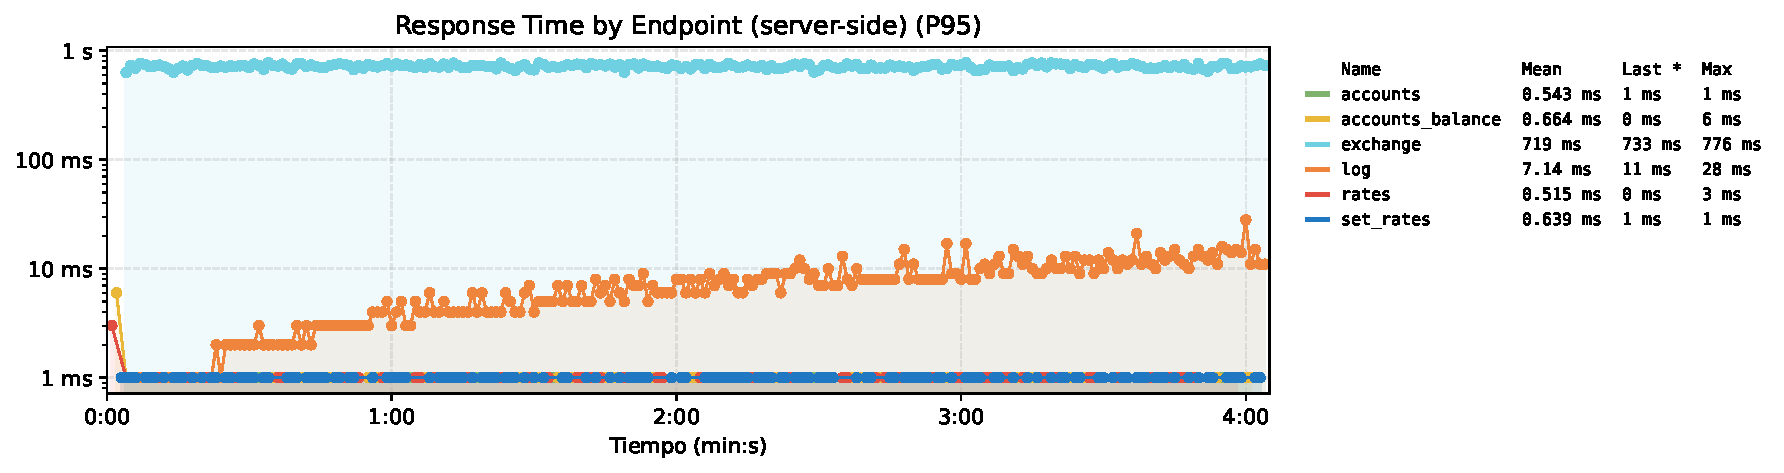
\includegraphics[width=0.8\columnwidth]{figures/propuesta_2/baseline/endpoint_response_time}
            \caption{
                Tiempo de respuesta por endpoint de la propuesta 2.
                El eje tiene una escala logarítmica.
            }
            \label{fig:resultados_completos_propuesta_2_baseline_endpoint_response_time}
        \end{figure}

        \begin{figure}[H]
            \centering
            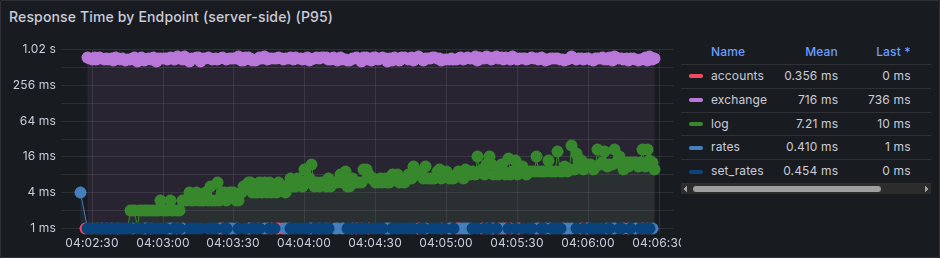
\includegraphics[width=0.8\columnwidth]{figures/propuesta_2/baseline/endpoint_response_time_captura}
            \caption{ Se adjunta la captura correspondiente a la Figura~\ref{fig:resultados_completos_propuesta_2_baseline_endpoint_response_time}. }
            \label{fig:resultados_completos_propuesta_2_baseline_endpoint_response_time_captura}
        \end{figure}

        \begin{figure}[H]
            \centering
            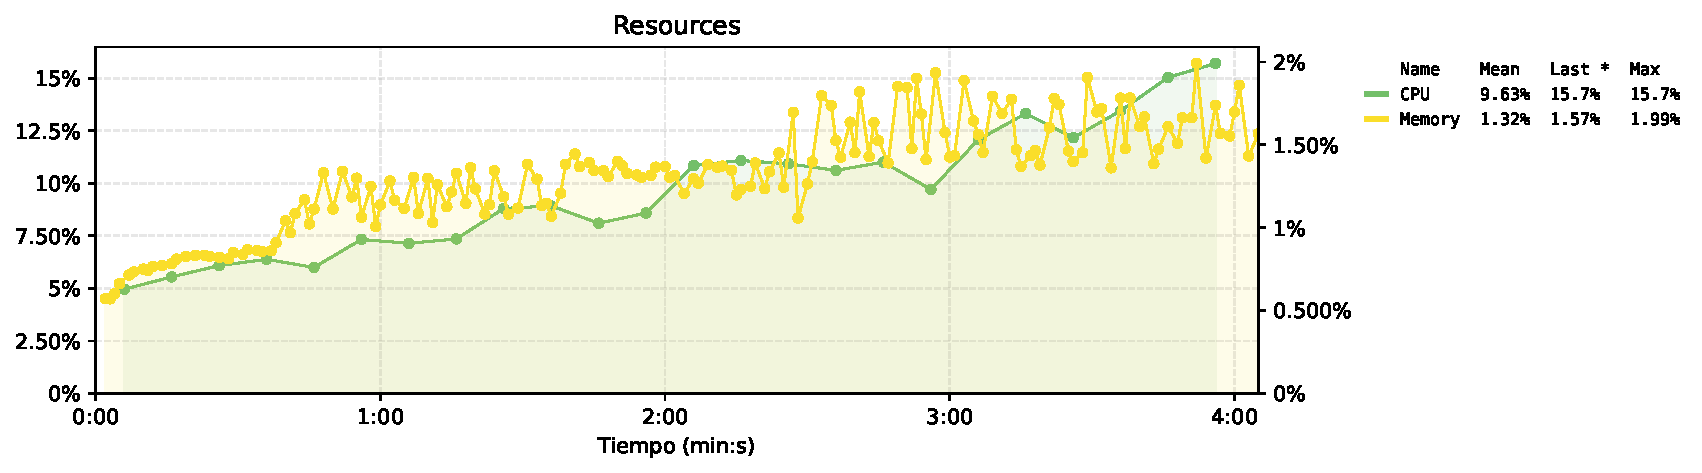
\includegraphics[width=0.8\columnwidth]{figures/propuesta_2/baseline/resources}
            \caption{
                Estado de los recursos de la propuesta 2.
                El eje izquierdo muestra el uso de CPU, el eje derecho muestra el uso de memoria.
            }
            \label{fig:resultados_completos_propuesta_2_baseline_resources}
        \end{figure}

        \begin{figure}[H]
            \centering
            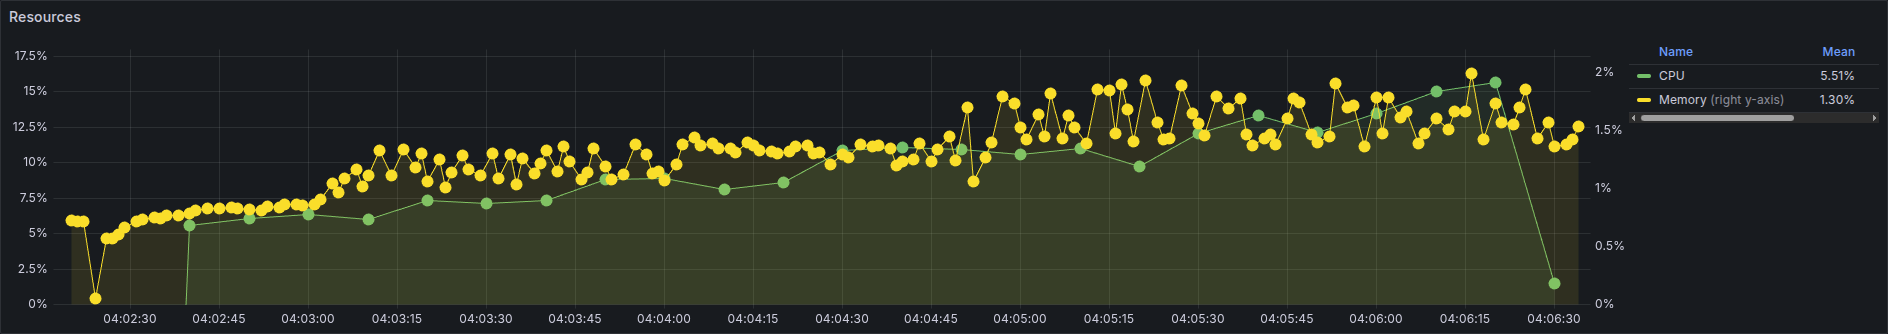
\includegraphics[width=0.8\columnwidth]{figures/propuesta_2/baseline/resources_captura}
            \caption{ Se adjunta la captura correspondiente a la Figura~\ref{fig:resultados_completos_propuesta_2_baseline_resources}. }
            \label{fig:resultados_completos_propuesta_2_baseline_resources_captura}
        \end{figure}

        \begin{figure}[H]
            \centering
            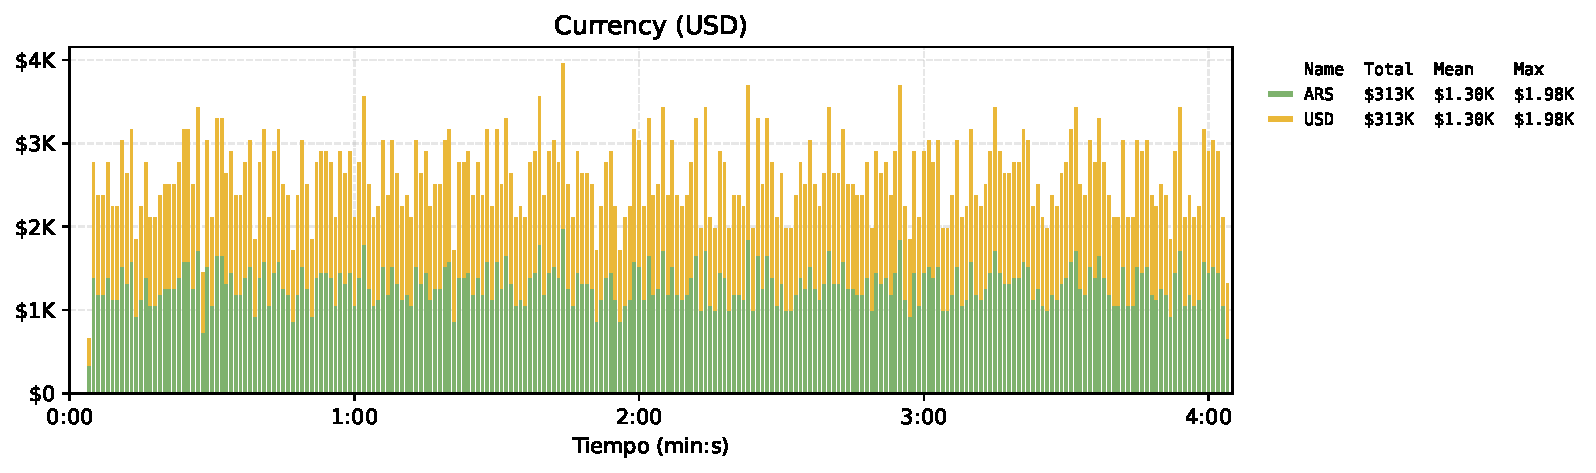
\includegraphics[width=0.8\columnwidth]{figures/propuesta_2/baseline/currency}
            \caption{ Volumen operado en cada moneda en la propuesta 2. }
            \label{fig:resultados_completos_propuesta_2_baseline_currency}
        \end{figure}

        \begin{figure}[H]
            \centering
            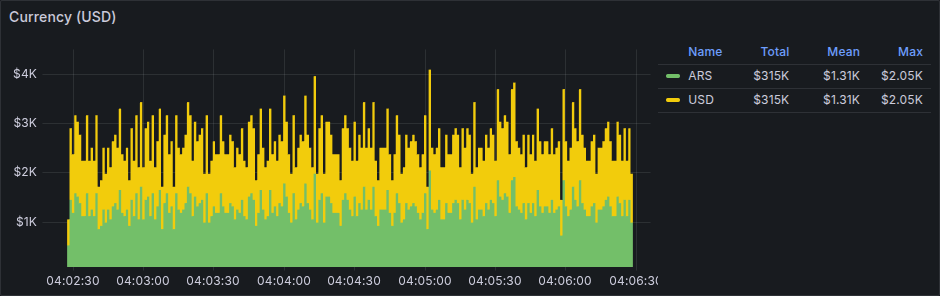
\includegraphics[width=0.8\columnwidth]{figures/propuesta_2/baseline/currency_captura}
            \caption{ Se adjunta la captura correspondiente a la Figura~\ref{fig:resultados_completos_propuesta_2_baseline_currency}. }
            \label{fig:resultados_completos_propuesta_2_baseline_currency_captura}
        \end{figure}

        \begin{figure}[H]
            \centering
            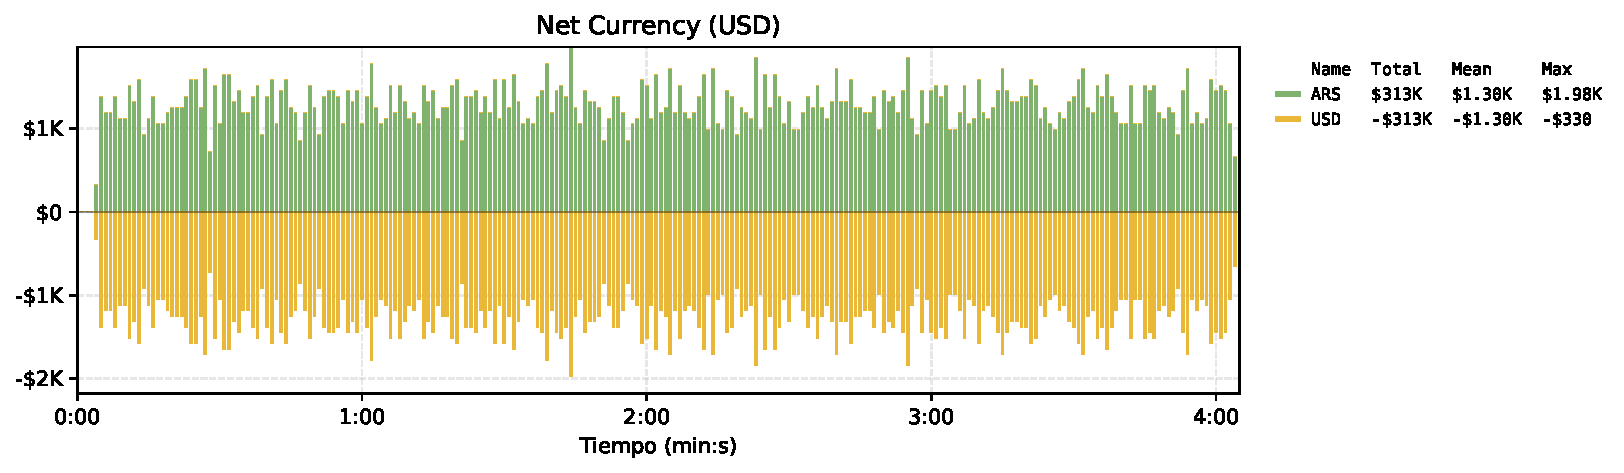
\includegraphics[width=0.8\columnwidth]{figures/propuesta_2/baseline/net_currency}
            \caption{ Neto operado en cada moneda en la propuesta 2. }
            \label{fig:resultados_completos_propuesta_2_baseline_net_currency}
        \end{figure}

        \begin{figure}[H]
            \centering
            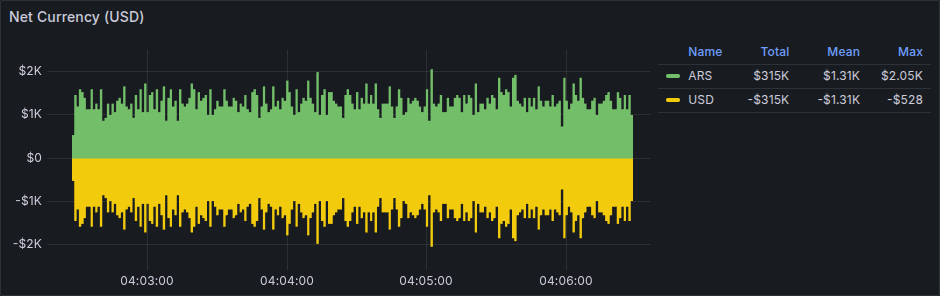
\includegraphics[width=0.8\columnwidth]{figures/propuesta_2/baseline/net_currency_captura}
            \caption{ Se adjunta la captura correspondiente a la Figura~\ref{fig:resultados_completos_propuesta_2_baseline_net_currency}. }
            \label{fig:resultados_completos_propuesta_2_baseline_net_currency_captura}
        \end{figure}

    \clearpage

    \subsection{Resultados completos del escenario de estrés sobre la propuesta 2}
    \label{sec:resultados_completos_propuesta_2_stress}

        \begin{figure}[H]
            \centering
            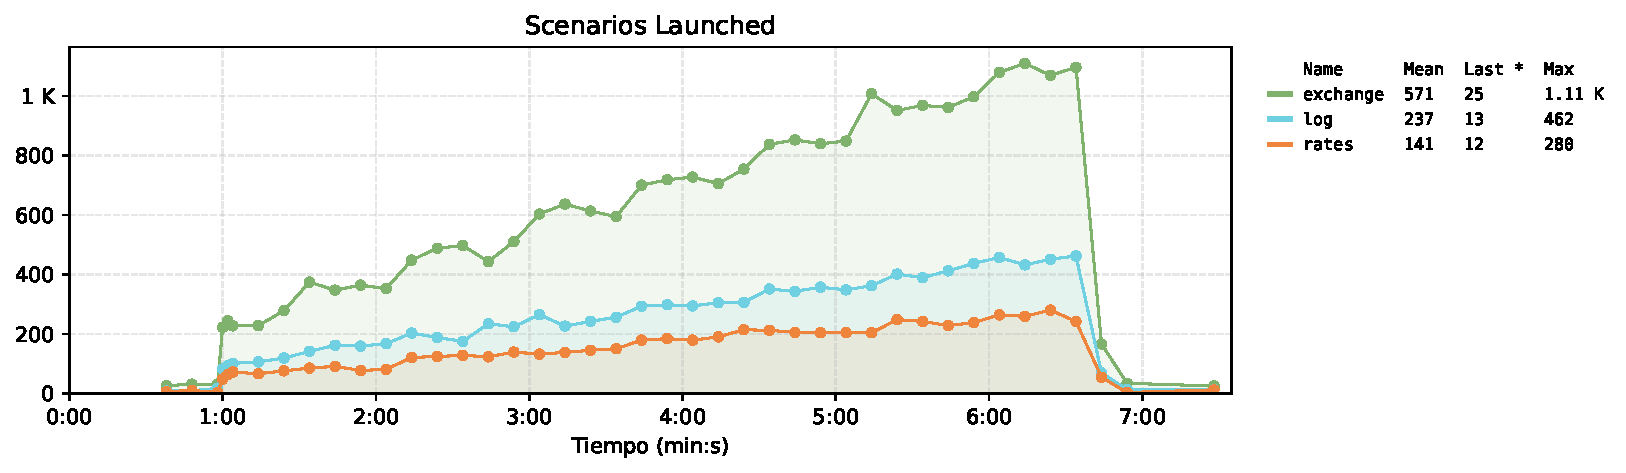
\includegraphics[width=0.8\columnwidth]{figures/propuesta_2/stress/scenarios}
            \caption{ Escenarios de la propuesta 2. }
            \label{fig:resultados_completos_propuesta_2_stress_scenarios}
        \end{figure}

        \begin{figure}[H]
            \centering
            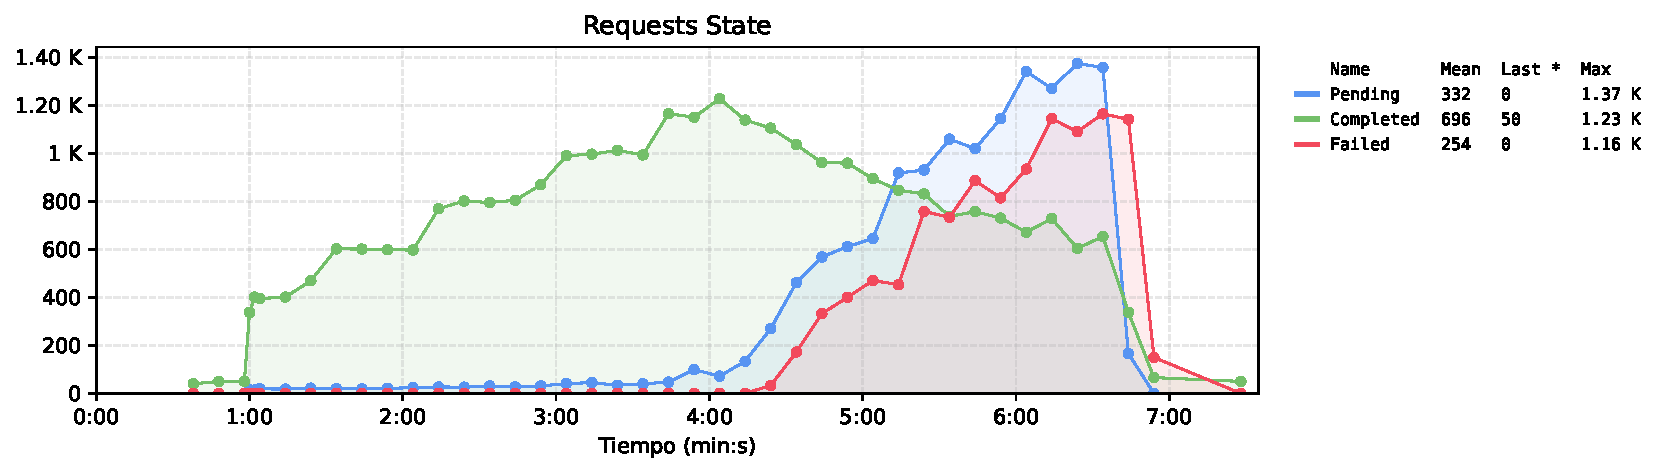
\includegraphics[width=0.8\columnwidth]{figures/propuesta_2/stress/requests_state}
            \caption{ Estado de las requests de la propuesta 2. }
            \label{fig:resultados_completos_propuesta_2_stress_requests_state}
        \end{figure}

        \begin{figure}[H]
            \centering
            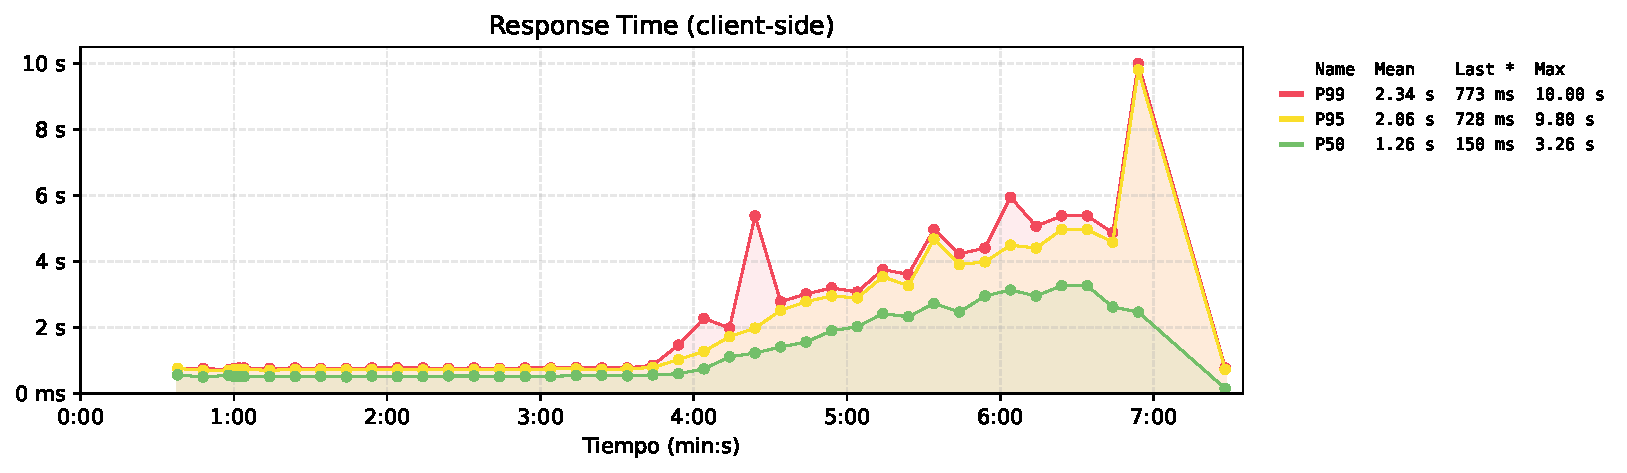
\includegraphics[width=0.8\columnwidth]{figures/propuesta_2/stress/response_time}
            \caption{ Tiempo de respuesta de la propuesta 2. }
            \label{fig:resultados_completos_propuesta_2_stress_response_time}
        \end{figure}

        \begin{figure}[H]
            \centering
            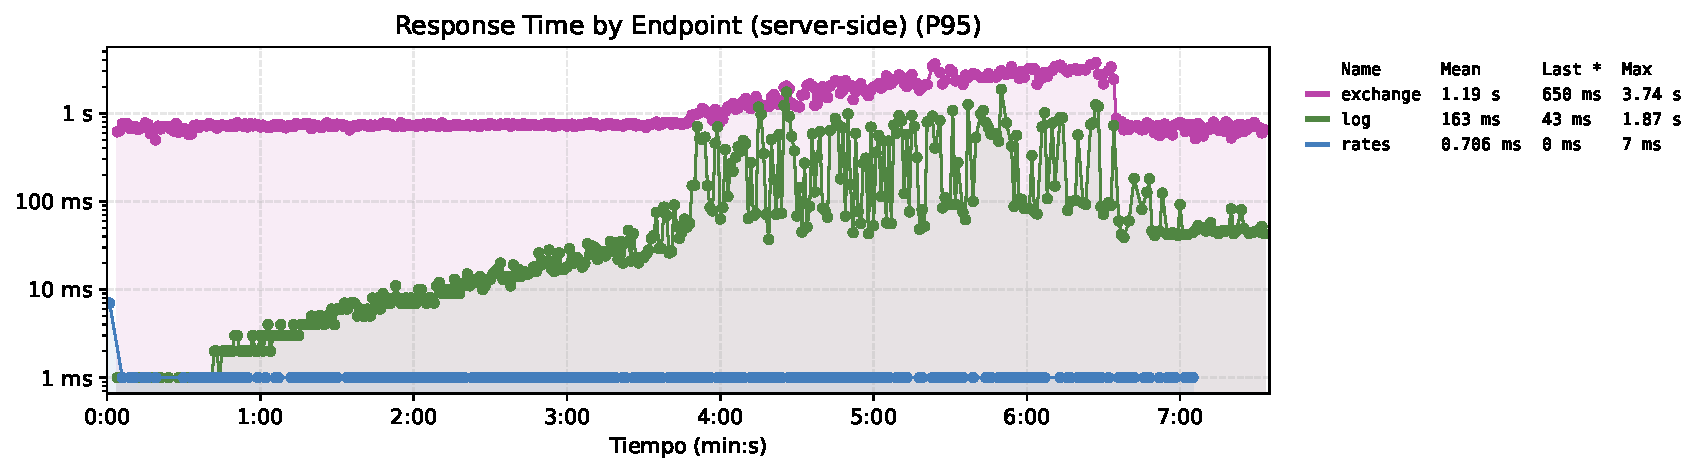
\includegraphics[width=0.8\columnwidth]{figures/propuesta_2/stress/endpoint_response_time}
            \caption{
                Tiempo de respuesta por endpoint de la propuesta 2.
                El eje tiene una escala logarítmica.
            }
            \label{fig:resultados_completos_propuesta_2_stress_endpoint_response_time}
        \end{figure}

        \begin{figure}[H]
            \centering
            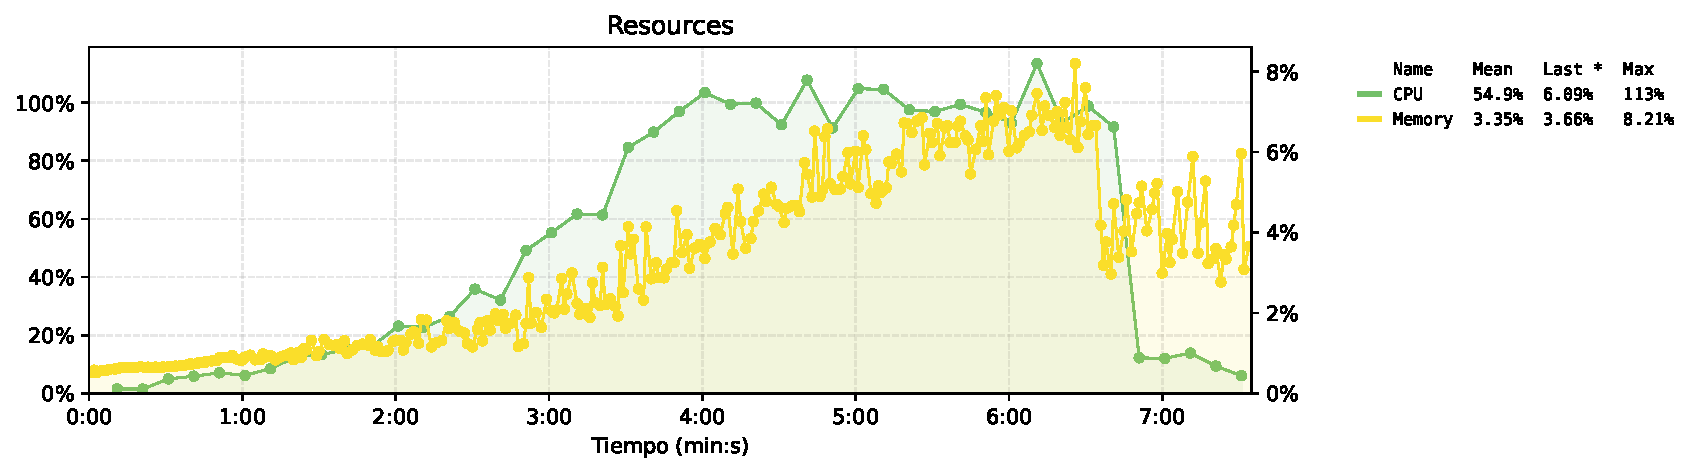
\includegraphics[width=0.8\columnwidth]{figures/propuesta_2/stress/resources}
            \caption{
                Estado de los recursos de la propuesta 2.
                El eje izquierdo muestra el uso de CPU, el eje derecho muestra el uso de memoria.
            }
            \label{fig:resultados_completos_propuesta_2_stress_resources}
        \end{figure}

        \begin{figure}[H]
            \centering
            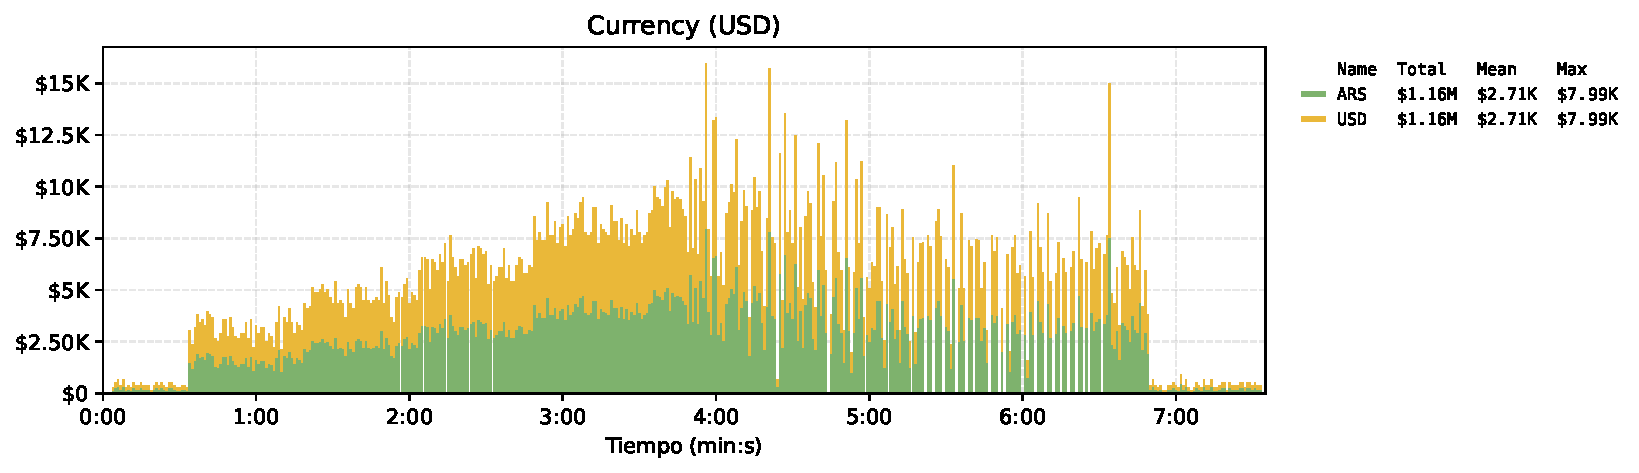
\includegraphics[width=0.8\columnwidth]{figures/propuesta_2/stress/currency}
            \caption{ Volumen operado en cada moneda en la propuesta 2. }
            \label{fig:resultados_completos_propuesta_2_stress_currency}
        \end{figure}

        \begin{figure}[H]
            \centering
            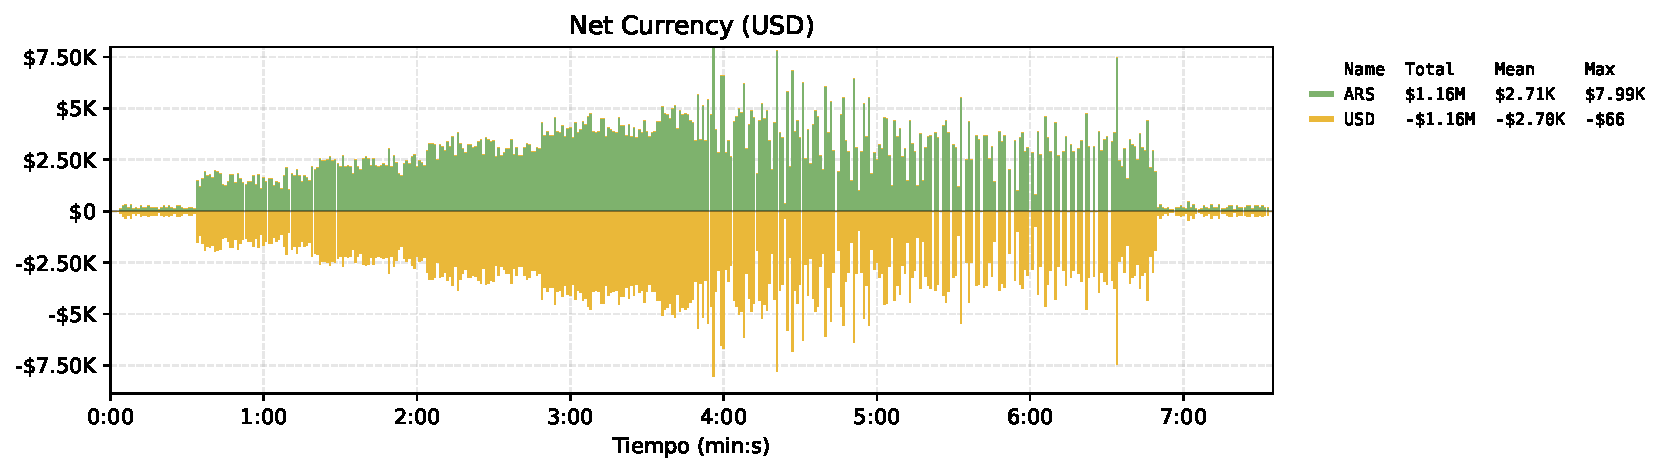
\includegraphics[width=0.8\columnwidth]{figures/propuesta_2/stress/net_currency}
            \caption{ Neto operado en cada moneda en la propuesta 2. }
            \label{fig:resultados_completos_propuesta_2_stress_net_currency}
        \end{figure}

    \clearpage

    \subsection{Resultados completos del escenario de resistencia sobre la propuesta 2}
    \label{sec:resultados_completos_propuesta_2_soak}

        \begin{figure}[H]
            \centering
            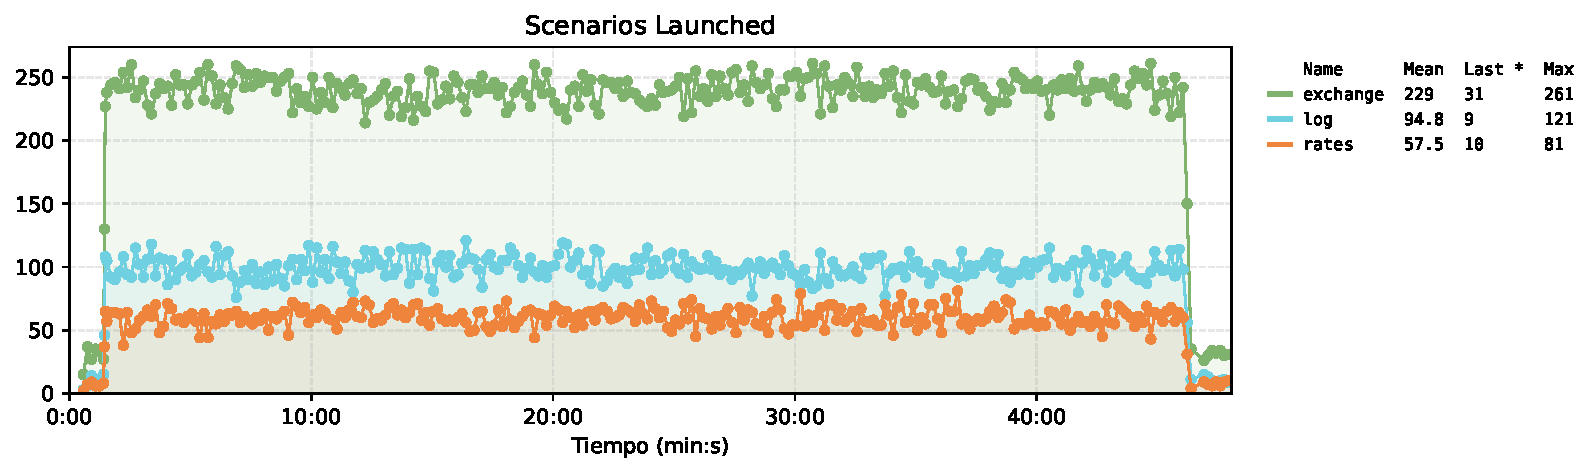
\includegraphics[width=0.8\columnwidth]{figures/propuesta_2/soak/scenarios}
            \caption{ Escenarios de la propuesta 2. }
            \label{fig:resultados_completos_propuesta_2_soak_scenarios}
        \end{figure}

        \begin{figure}[H]
            \centering
            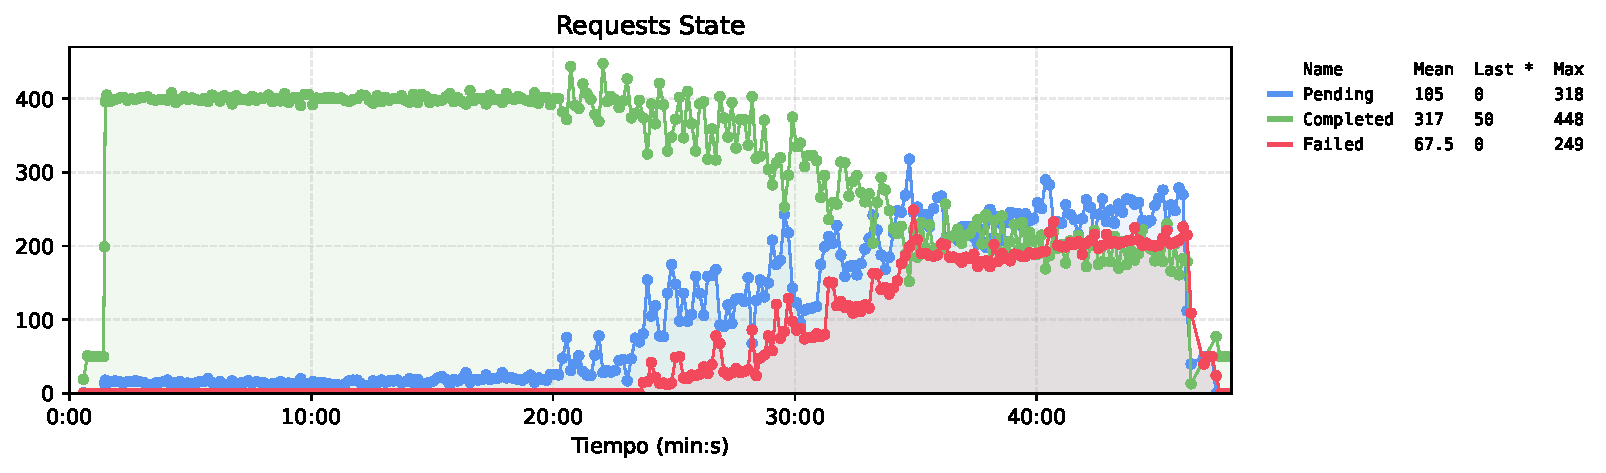
\includegraphics[width=0.8\columnwidth]{figures/propuesta_2/soak/requests_state}
            \caption{ Estado de las requests de la propuesta 2. }
            \label{fig:resultados_completos_propuesta_2_soak_requests_state}
        \end{figure}

        \begin{figure}[H]
            \centering
            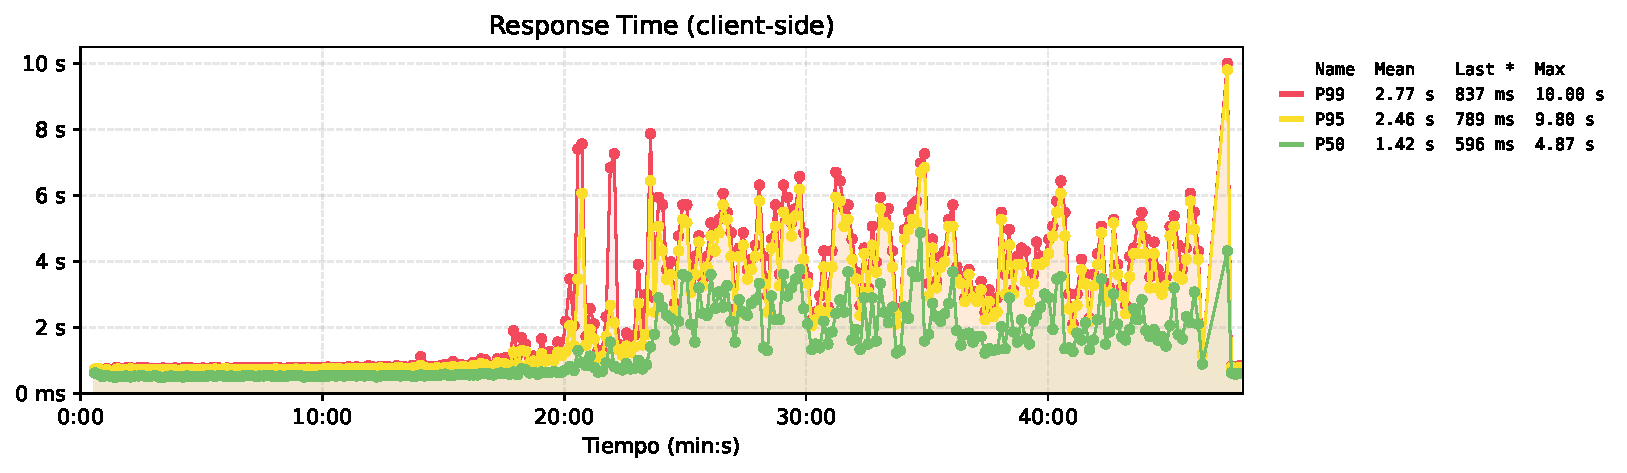
\includegraphics[width=0.8\columnwidth]{figures/propuesta_2/soak/response_time}
            \caption{ Tiempo de respuesta de la propuesta 2. }
            \label{fig:resultados_completos_propuesta_2_soak_response_time}
        \end{figure}

        \begin{figure}[H]
            \centering
            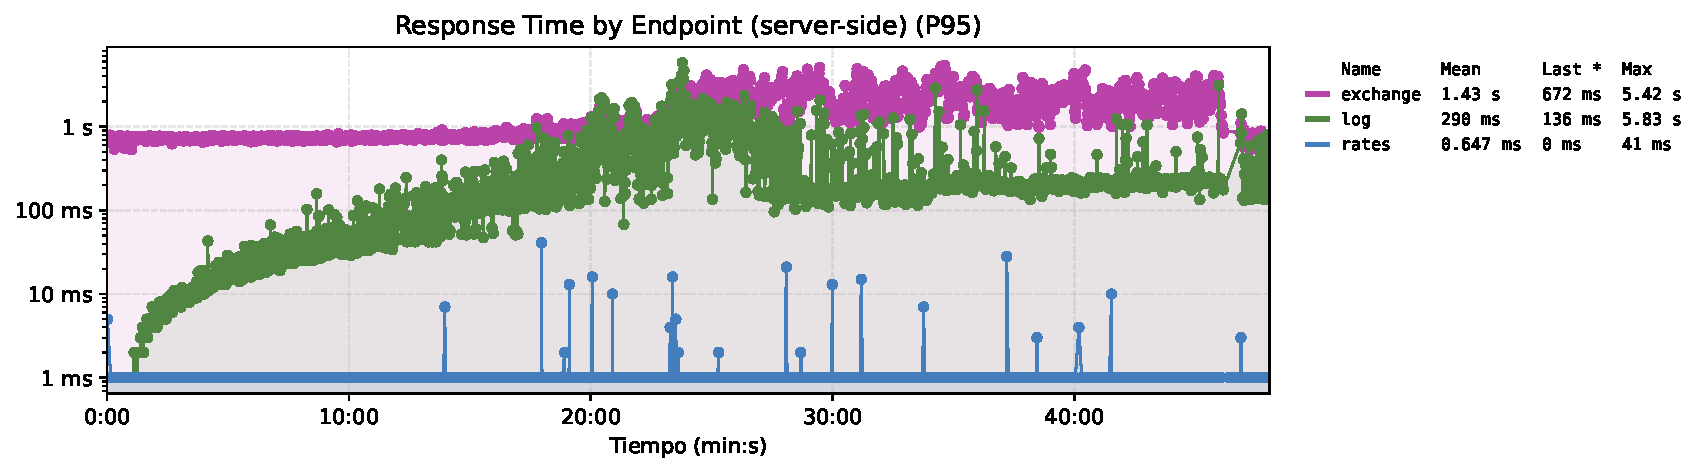
\includegraphics[width=0.8\columnwidth]{figures/propuesta_2/soak/endpoint_response_time}
            \caption{
                Tiempo de respuesta por endpoint de la propuesta 2.
                El eje tiene una escala logarítmica.
            }
            \label{fig:resultados_completos_propuesta_2_soak_endpoint_response_time}
        \end{figure}

        \begin{figure}[H]
            \centering
            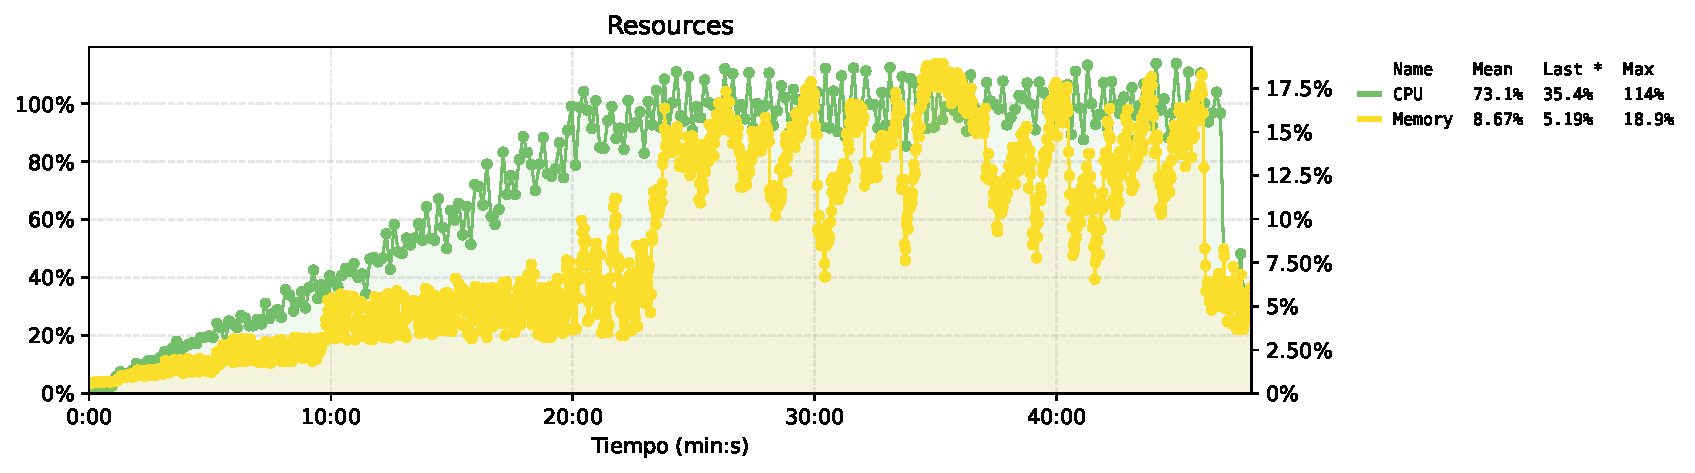
\includegraphics[width=0.8\columnwidth]{figures/propuesta_2/soak/resources}
            \caption{
                Estado de los recursos de la propuesta 2.
                El eje izquierdo muestra el uso de CPU, el eje derecho muestra el uso de memoria.
            }
            \label{fig:resultados_completos_propuesta_2_soak_resources}
        \end{figure}

        \begin{figure}[H]
            \centering
            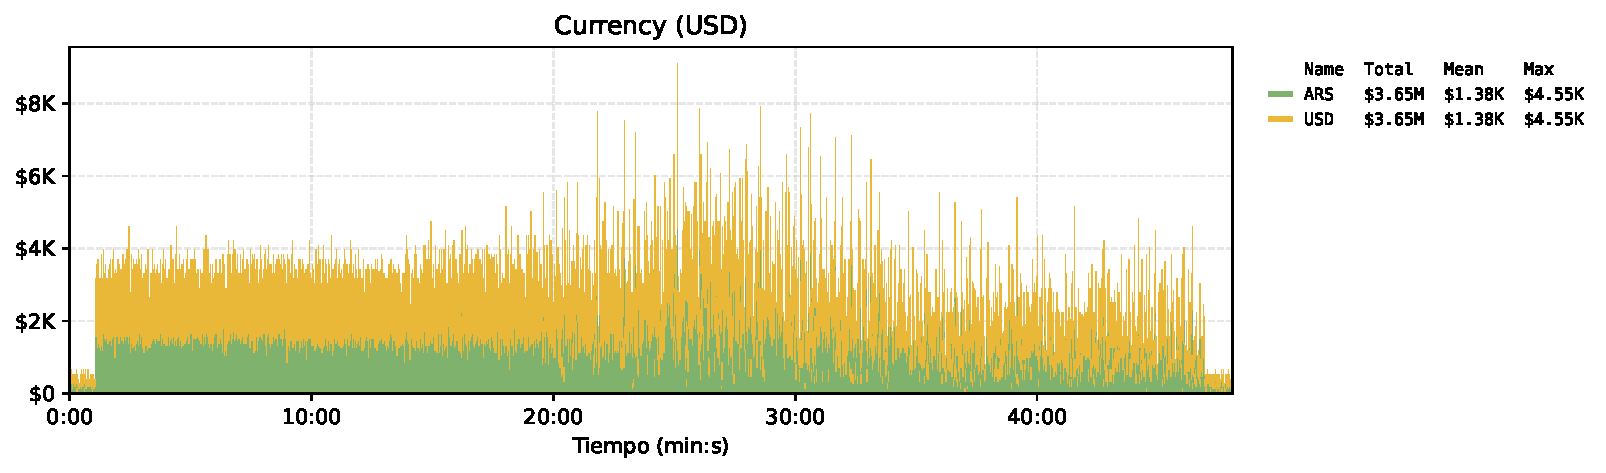
\includegraphics[width=0.8\columnwidth]{figures/propuesta_2/soak/currency}
            \caption{ Volumen operado en cada moneda en la propuesta 2. }
            \label{fig:resultados_completos_propuesta_2_soak_currency}
        \end{figure}

        \begin{figure}[H]
            \centering
            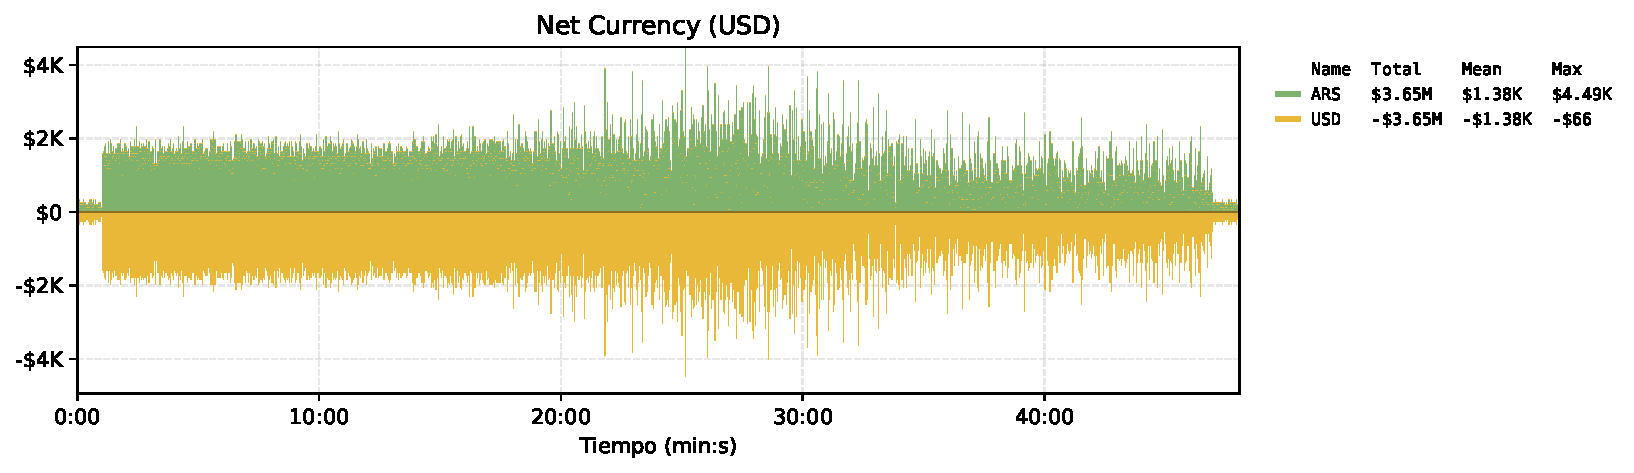
\includegraphics[width=0.8\columnwidth]{figures/propuesta_2/soak/net_currency}
            \caption{ Neto operado en cada moneda en la propuesta 2. }
            \label{fig:resultados_completos_propuesta_2_soak_net_currency}
        \end{figure}

    \clearpage

    \subsection{Resultados completos del escenario de caos sobre la propuesta 2}
    \label{sec:resultados_completos_propuesta_2_chaos}

        \begin{figure}[H]
            \centering
            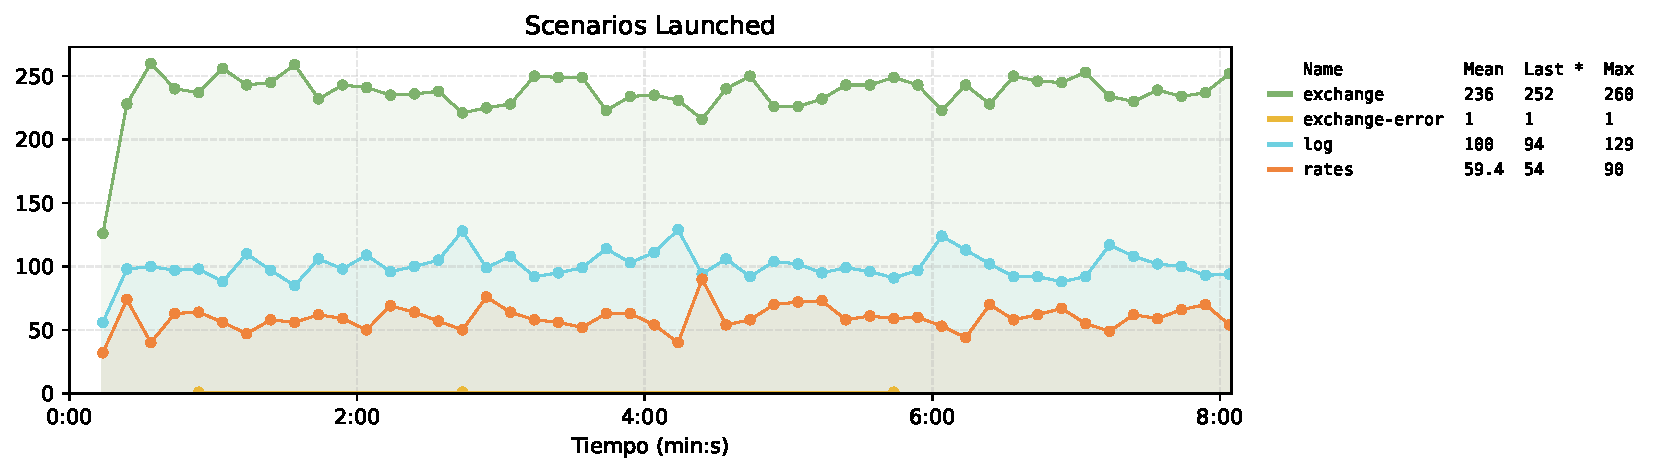
\includegraphics[width=0.8\columnwidth]{figures/propuesta_2/chaos/scenarios}
            \caption{ Escenarios de la propuesta 2. }
            \label{fig:resultados_completos_propuesta_2_chaos_scenarios}
        \end{figure}

        \begin{figure}[H]
            \centering
            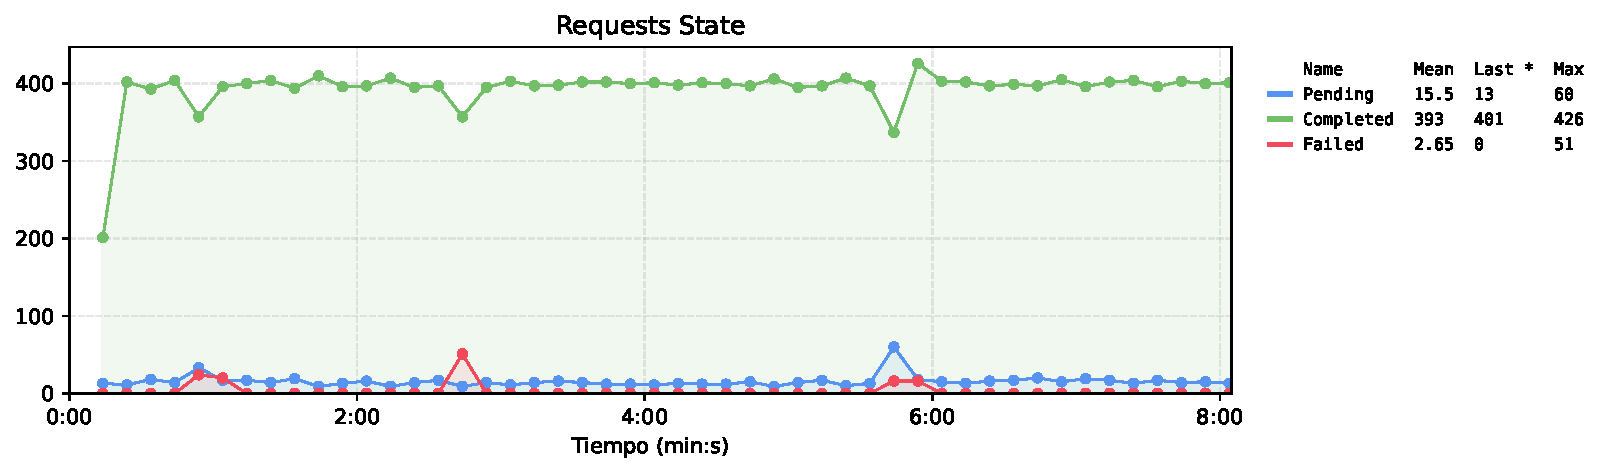
\includegraphics[width=0.8\columnwidth]{figures/propuesta_2/chaos/requests_state}
            \caption{ Estado de las requests de la propuesta 2. }
            \label{fig:resultados_completos_propuesta_2_chaos_requests_state}
        \end{figure}

        \begin{figure}[H]
            \centering
            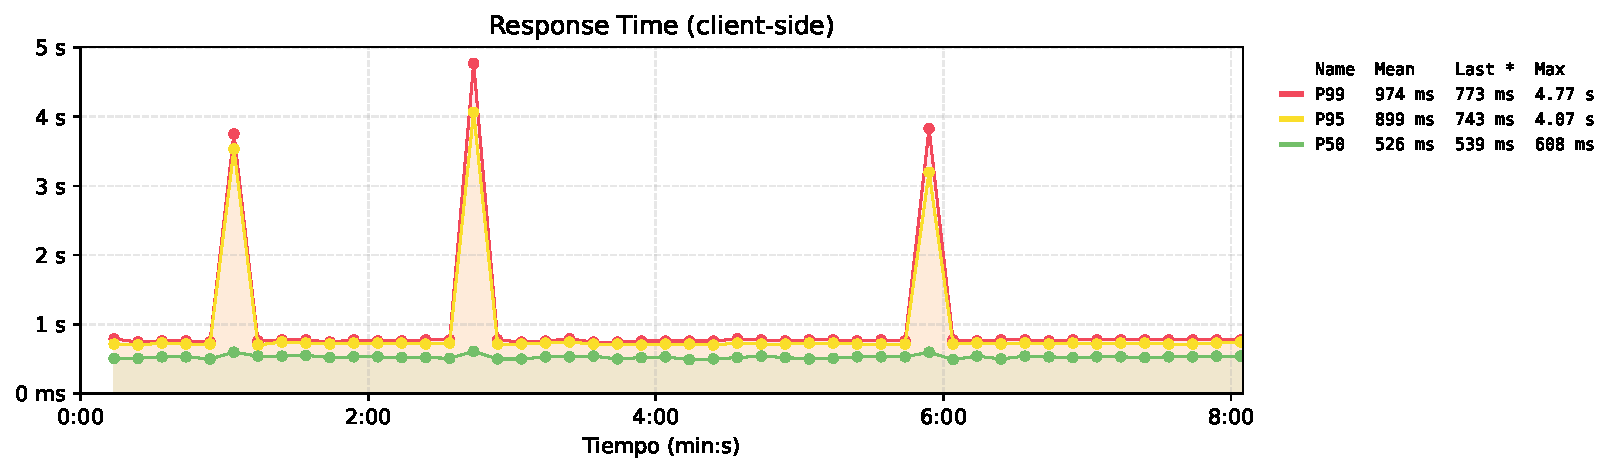
\includegraphics[width=0.8\columnwidth]{figures/propuesta_2/chaos/response_time}
            \caption{ Tiempo de respuesta de la propuesta 2. }
            \label{fig:resultados_completos_propuesta_2_chaos_response_time}
        \end{figure}

        \begin{figure}[H]
            \centering
            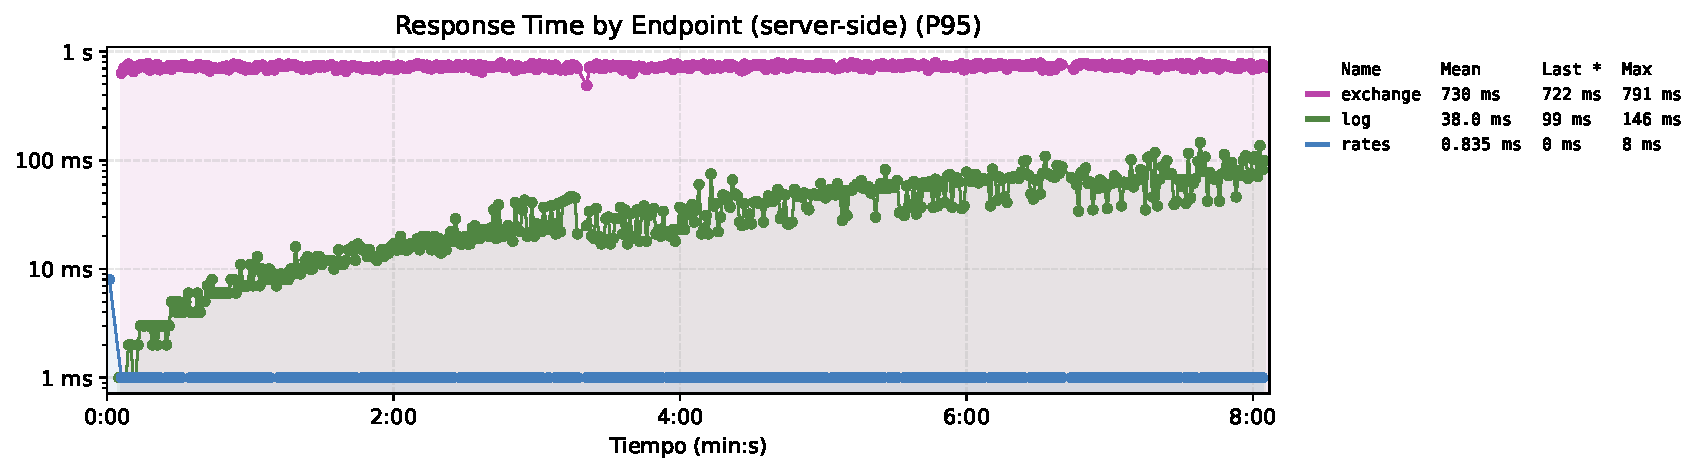
\includegraphics[width=0.8\columnwidth]{figures/propuesta_2/chaos/endpoint_response_time}
            \caption{
                Tiempo de respuesta por endpoint de la propuesta 2.
                El eje tiene una escala logarítmica.
            }
            \label{fig:resultados_completos_propuesta_2_chaos_endpoint_response_time}
        \end{figure}

        \begin{figure}[H]
            \centering
            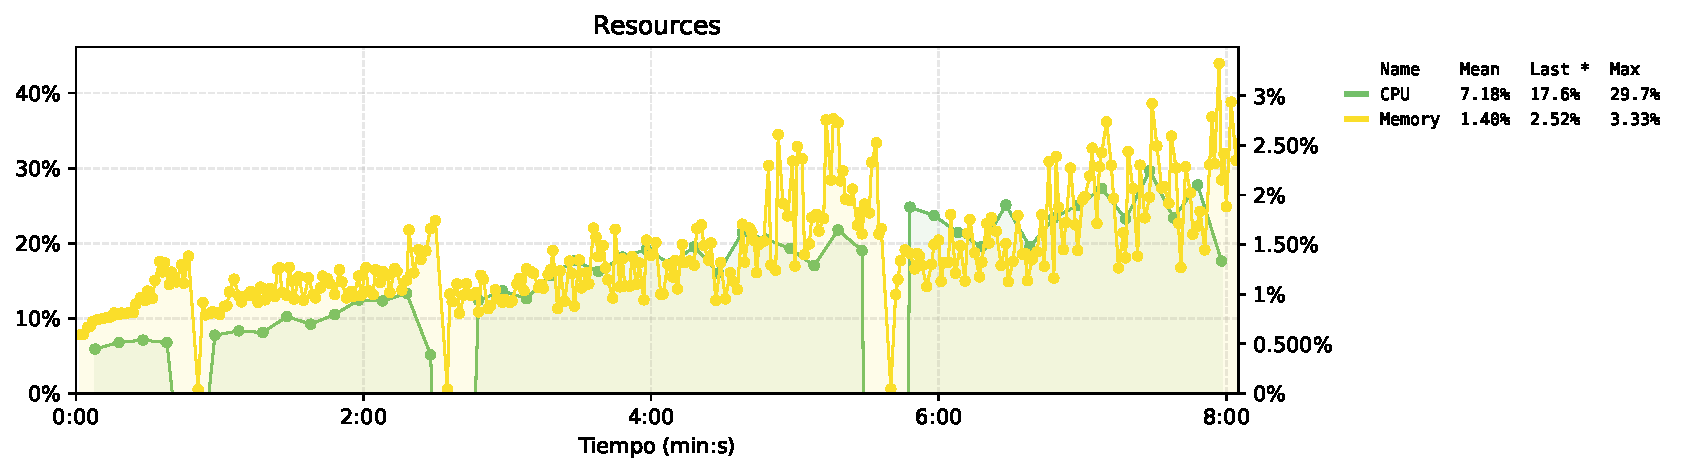
\includegraphics[width=0.8\columnwidth]{figures/propuesta_2/chaos/resources}
            \caption{
                Estado de los recursos de la propuesta 2.
                El eje izquierdo muestra el uso de CPU, el eje derecho muestra el uso de memoria.
            }
            \label{fig:resultados_completos_propuesta_2_chaos_resources}
        \end{figure}

        \begin{figure}[H]
            \centering
            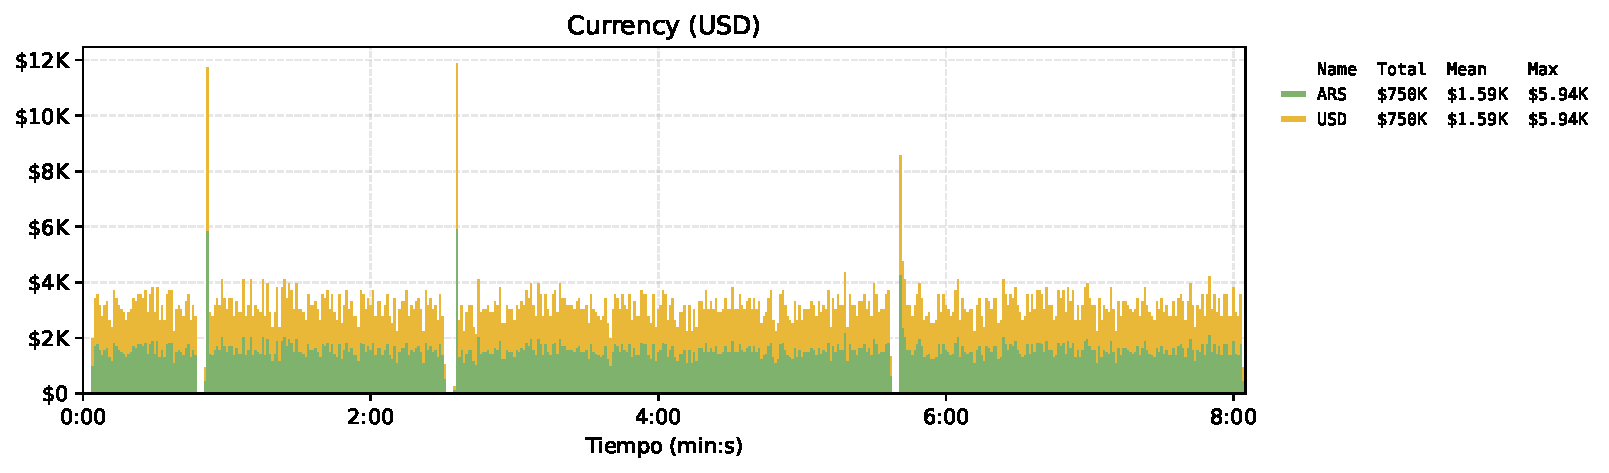
\includegraphics[width=0.8\columnwidth]{figures/propuesta_2/chaos/currency}
            \caption{ Volumen operado en cada moneda en la propuesta 2. }
            \label{fig:resultados_completos_propuesta_2_chaos_currency}
        \end{figure}

        \begin{figure}[H]
            \centering
            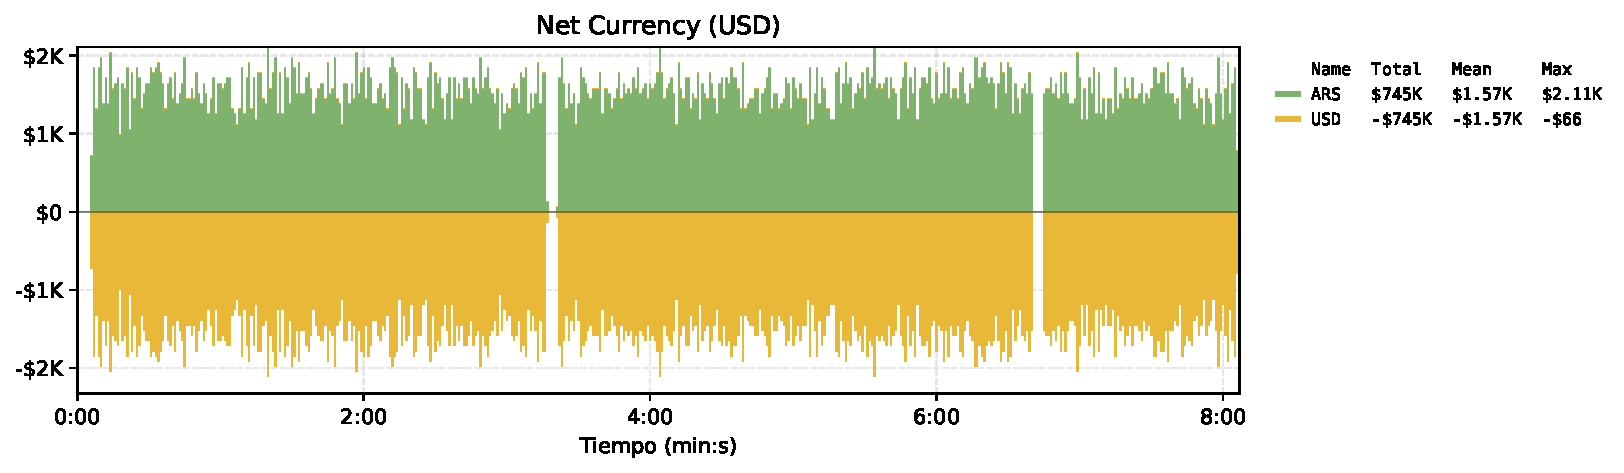
\includegraphics[width=0.8\columnwidth]{figures/propuesta_2/chaos/net_currency}
            \caption{ Neto operado en cada moneda en la propuesta 2. }
            \label{fig:resultados_completos_propuesta_2_chaos_net_currency}
        \end{figure}

    \clearpage

    \subsection{Resultados completos del escenario de estrés sobre la propuesta 3}
    \label{sec:resultados_completos_propuesta_3_stress}

        \begin{figure}[H]
            \centering
            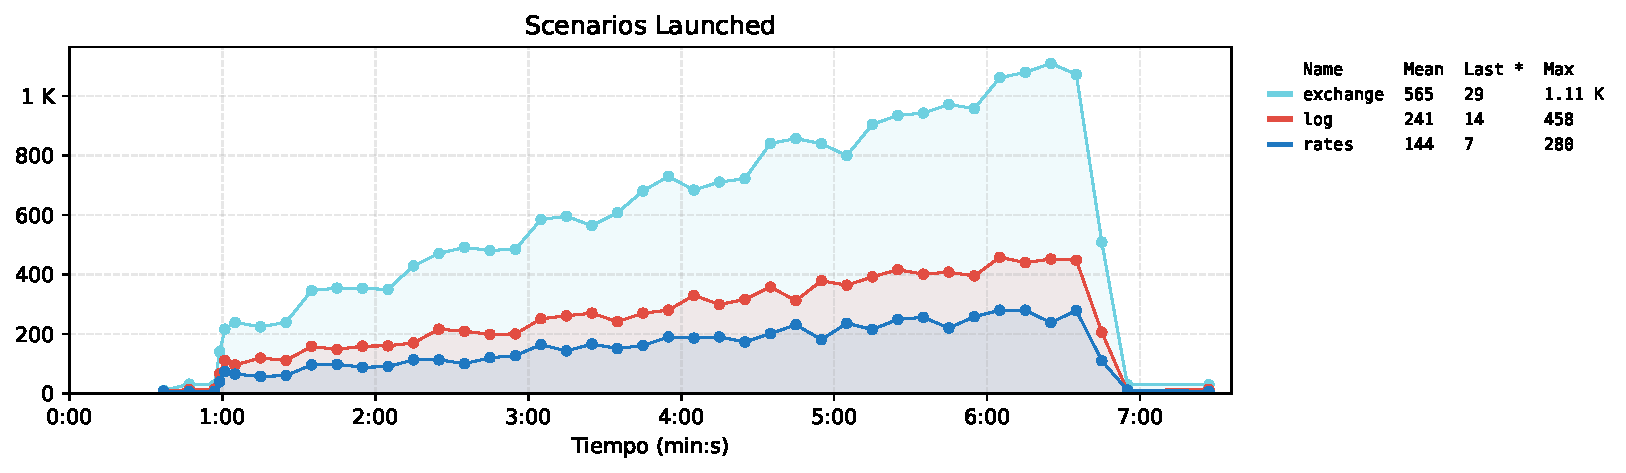
\includegraphics[width=0.8\columnwidth]{figures/propuesta_3/stress/scenarios}
            \caption{ Escenarios de la propuesta 3. }
            \label{fig:resultados_completos_propuesta_3_stress_scenarios}
        \end{figure}

        \begin{figure}[H]
            \centering
            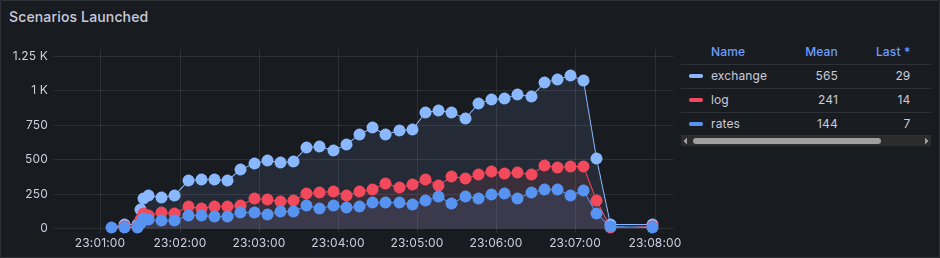
\includegraphics[width=0.8\columnwidth]{figures/propuesta_3/stress/scenarios_captura}
            \caption{ Se adjunta la captura correspondiente a la Figura~\ref{fig:resultados_completos_propuesta_3_stress_scenarios}. }
            \label{fig:resultados_completos_propuesta_3_stress_scenarios_captura}
        \end{figure}

        \begin{figure}[H]
            \centering
            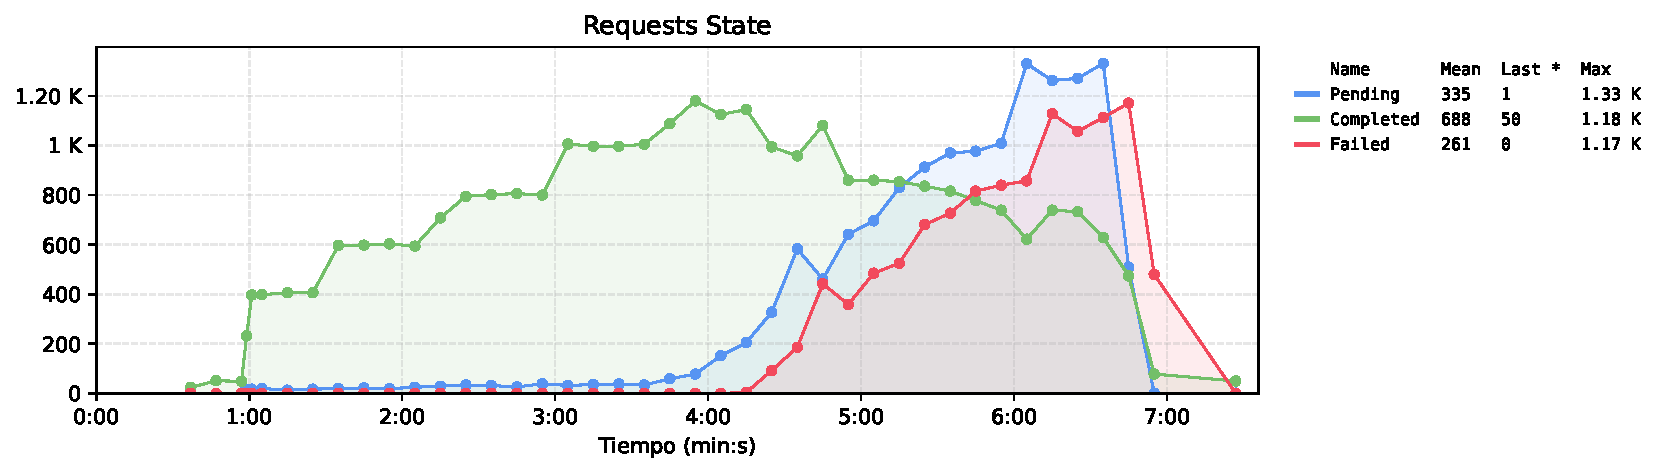
\includegraphics[width=0.8\columnwidth]{figures/propuesta_3/stress/requests_state}
            \caption{ Estado de las requests de la propuesta 3. }
            \label{fig:resultados_completos_propuesta_3_stress_requests_state}
        \end{figure}

        \begin{figure}[H]
            \centering
            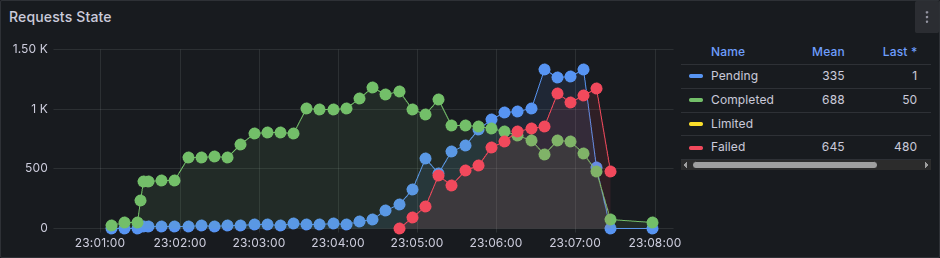
\includegraphics[width=0.8\columnwidth]{figures/propuesta_3/stress/requests_state_captura}
            \caption{ Se adjunta la captura correspondiente a la Figura~\ref{fig:resultados_completos_propuesta_3_stress_requests_state}. }
            \label{fig:resultados_completos_propuesta_3_stress_requests_state_captura}
        \end{figure}

        \begin{figure}[H]
            \centering
            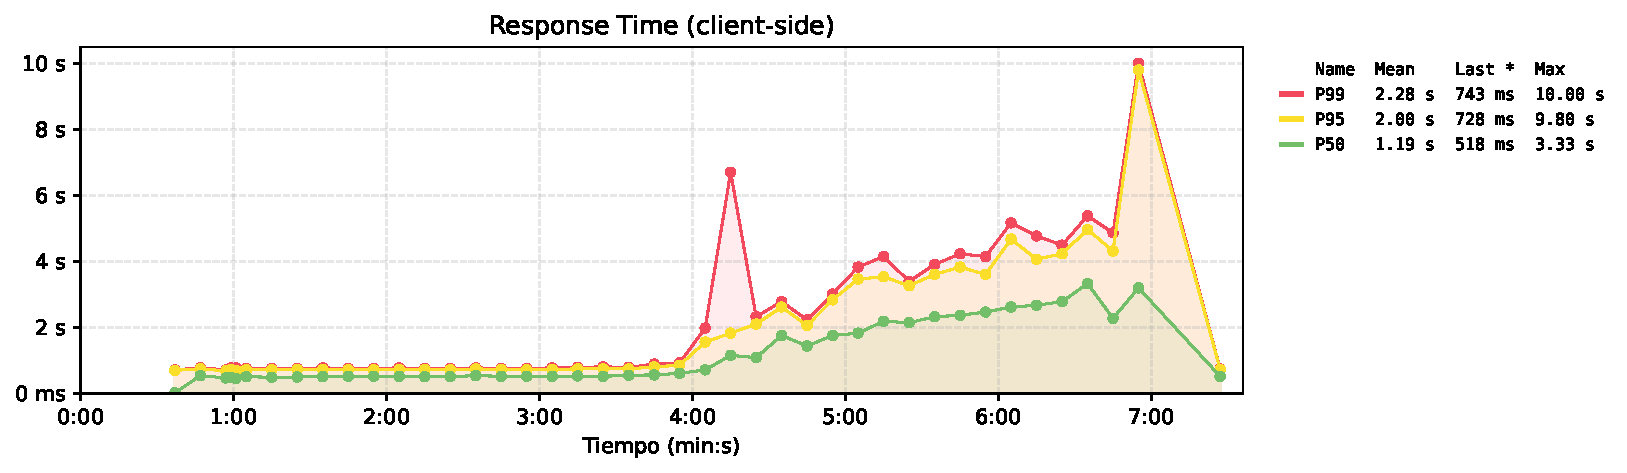
\includegraphics[width=0.8\columnwidth]{figures/propuesta_3/stress/response_time}
            \caption{ Tiempo de respuesta de la propuesta 3. }
            \label{fig:resultados_completos_propuesta_3_stress_response_time}
        \end{figure}

        \begin{figure}[H]
            \centering
            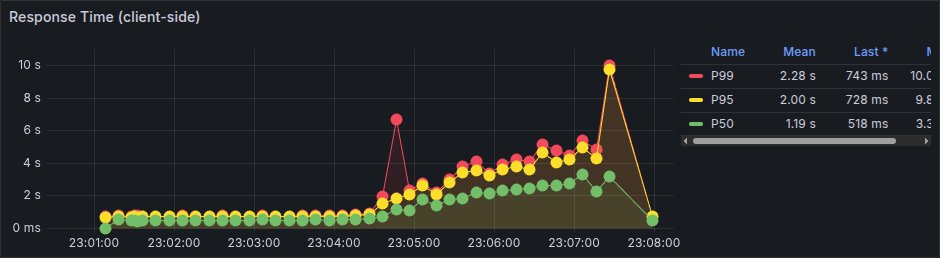
\includegraphics[width=0.8\columnwidth]{figures/propuesta_3/stress/response_time_captura}
            \caption{ Se adjunta la captura correspondiente a la Figura~\ref{fig:resultados_completos_propuesta_3_stress_response_time}. }
            \label{fig:resultados_completos_propuesta_3_stress_response_time_captura}
        \end{figure}

        \begin{figure}[H]
            \centering
            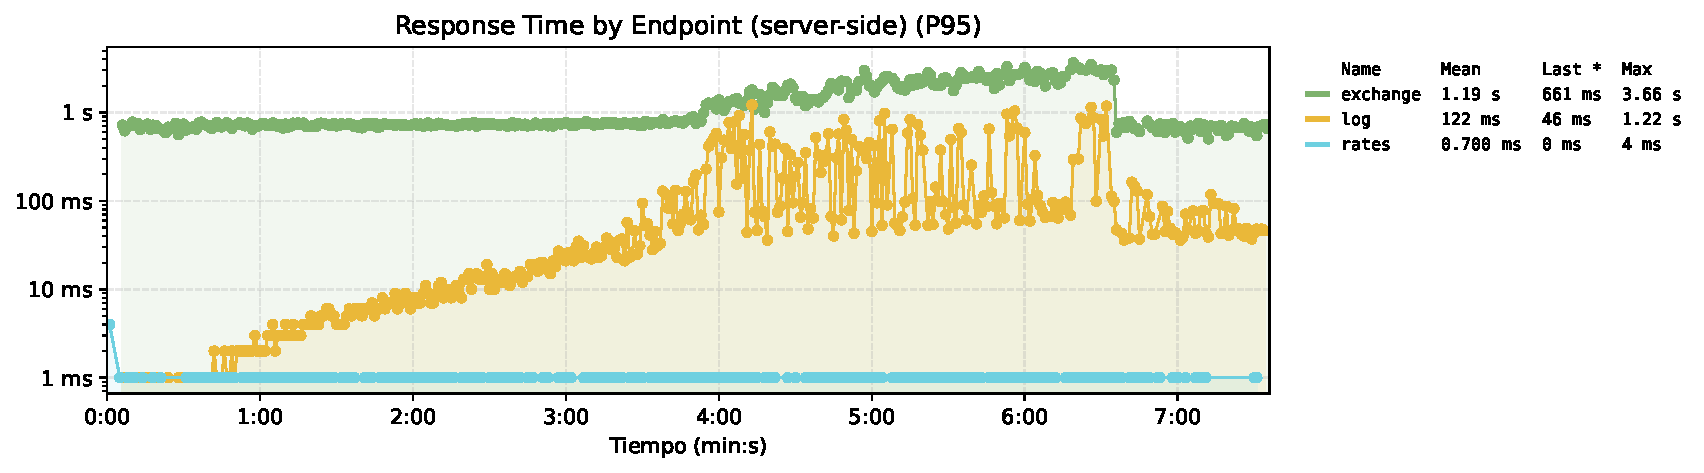
\includegraphics[width=0.8\columnwidth]{figures/propuesta_3/stress/endpoint_response_time}
            \caption{
                Tiempo de respuesta por endpoint de la propuesta 3.
                El eje tiene una escala logarítmica.
            }
            \label{fig:resultados_completos_propuesta_3_stress_endpoint_response_time}
        \end{figure}

        \begin{figure}[H]
            \centering
            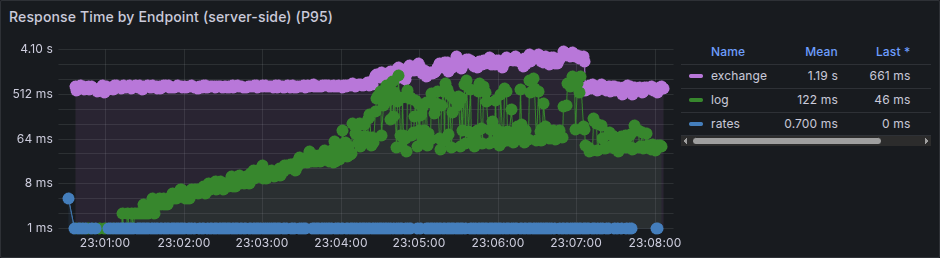
\includegraphics[width=0.8\columnwidth]{figures/propuesta_3/stress/endpoint_response_time_captura}
            \caption{ Se adjunta la captura correspondiente a la Figura~\ref{fig:resultados_completos_propuesta_3_stress_endpoint_response_time}. }
            \label{fig:resultados_completos_propuesta_3_stress_endpoint_response_time_captura}
        \end{figure}

        \begin{figure}[H]
            \centering
            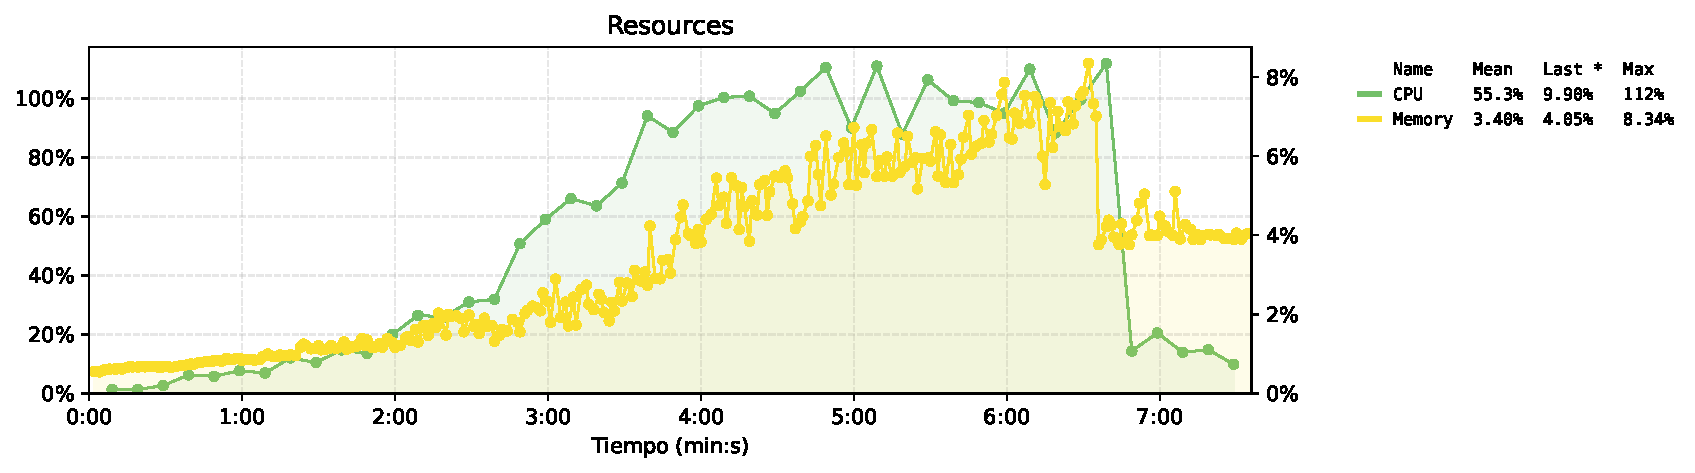
\includegraphics[width=0.8\columnwidth]{figures/propuesta_3/stress/resources}
            \caption{
                Estado de los recursos de la propuesta 3.
                El eje izquierdo muestra el uso de CPU, el eje derecho muestra el uso de memoria.
            }
            \label{fig:resultados_completos_propuesta_3_stress_resources}
        \end{figure}

        \begin{figure}[H]
            \centering
            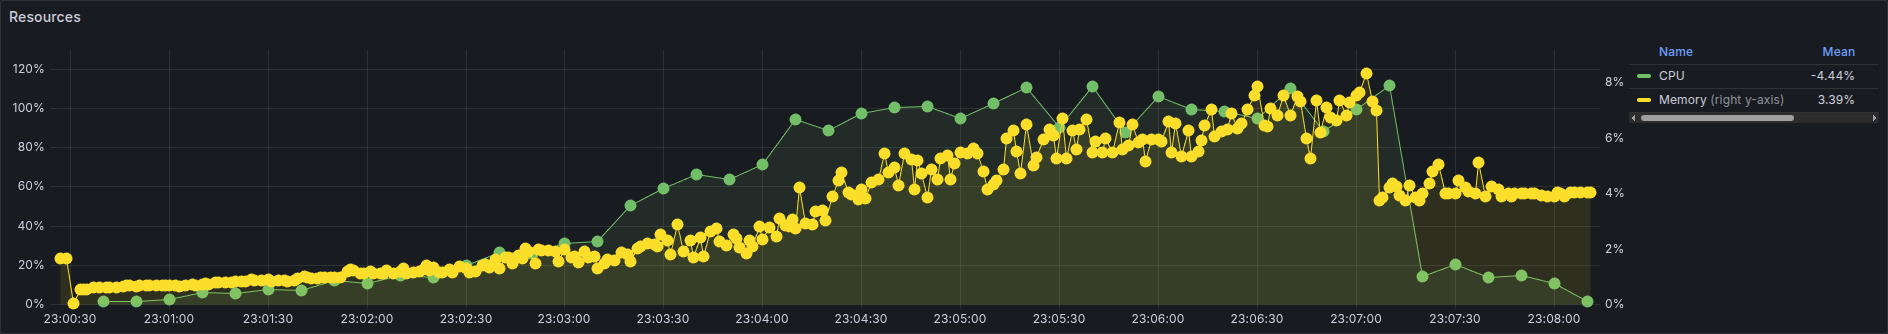
\includegraphics[width=0.8\columnwidth]{figures/propuesta_3/stress/resources_captura}
            \caption{ Se adjunta la captura correspondiente a la Figura~\ref{fig:resultados_completos_propuesta_3_stress_resources}. }
            \label{fig:resultados_completos_propuesta_3_stress_resources_captura}
        \end{figure}

        \begin{figure}[H]
            \centering
            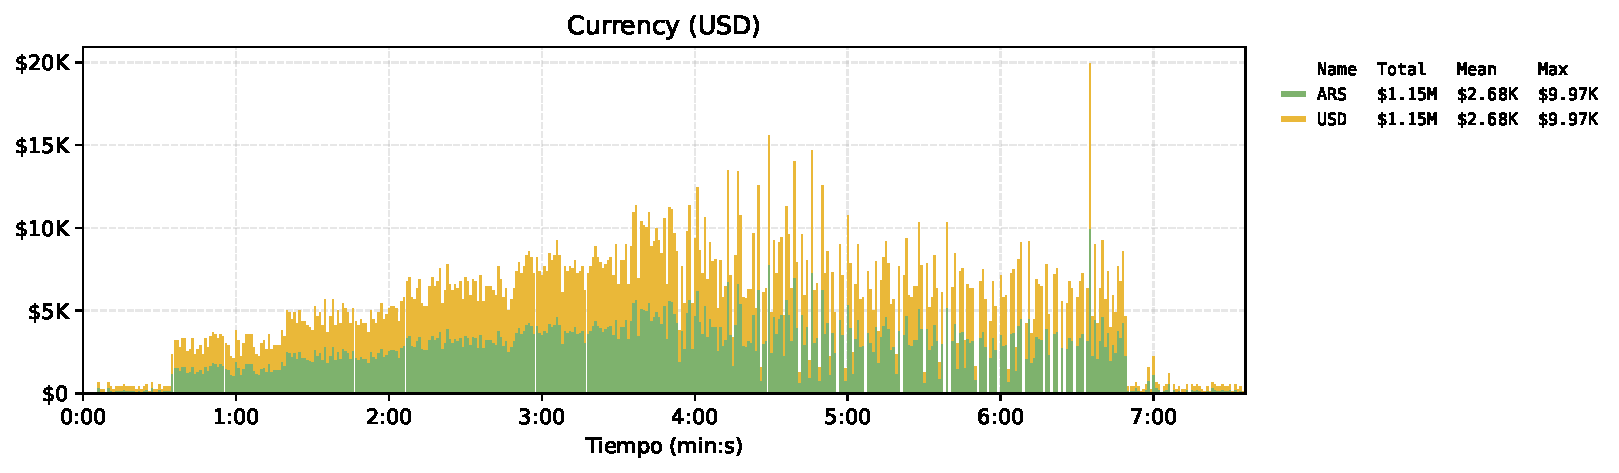
\includegraphics[width=0.8\columnwidth]{figures/propuesta_3/stress/currency}
            \caption{ Volumen operado en cada moneda en la propuesta 3. }
            \label{fig:resultados_completos_propuesta_3_stress_currency}
        \end{figure}

        \begin{figure}[H]
            \centering
            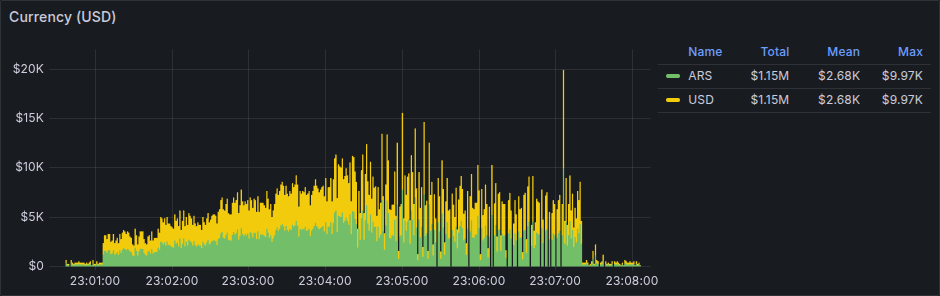
\includegraphics[width=0.8\columnwidth]{figures/propuesta_3/stress/currency_captura}
            \caption{ Se adjunta la captura correspondiente a la Figura~\ref{fig:resultados_completos_propuesta_3_stress_currency}. }
            \label{fig:resultados_completos_propuesta_3_stress_currency_captura}
        \end{figure}

        \begin{figure}[H]
            \centering
            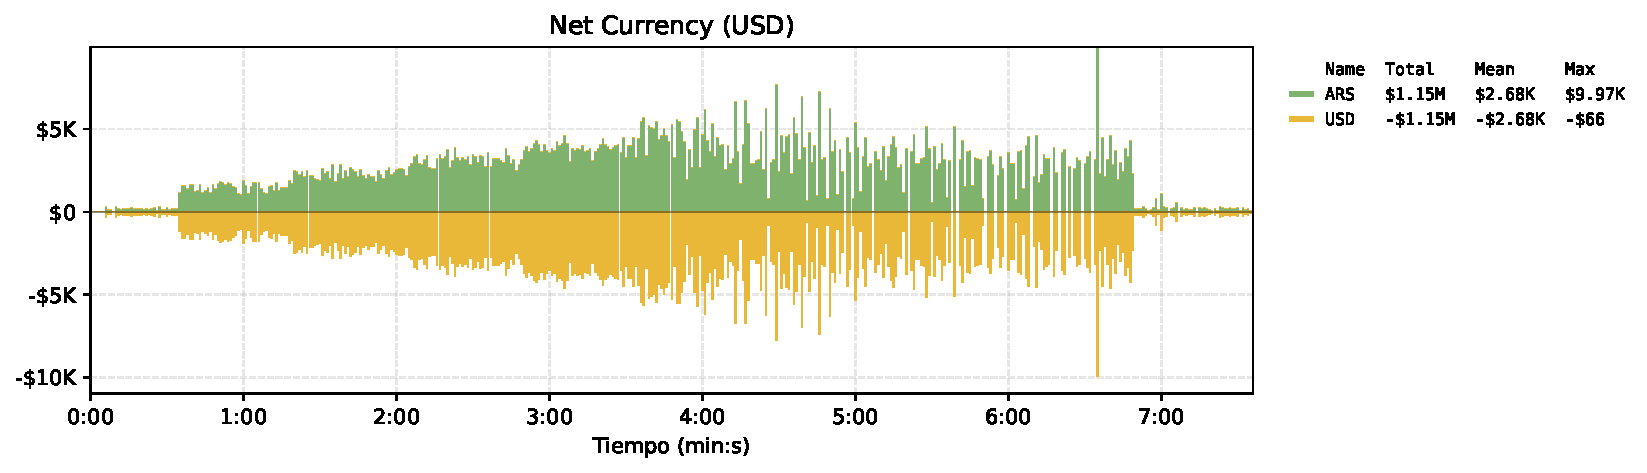
\includegraphics[width=0.8\columnwidth]{figures/propuesta_3/stress/net_currency}
            \caption{ Neto operado en cada moneda en la propuesta 3. }
            \label{fig:resultados_completos_propuesta_3_stress_net_currency}
        \end{figure}

        \begin{figure}[H]
            \centering
            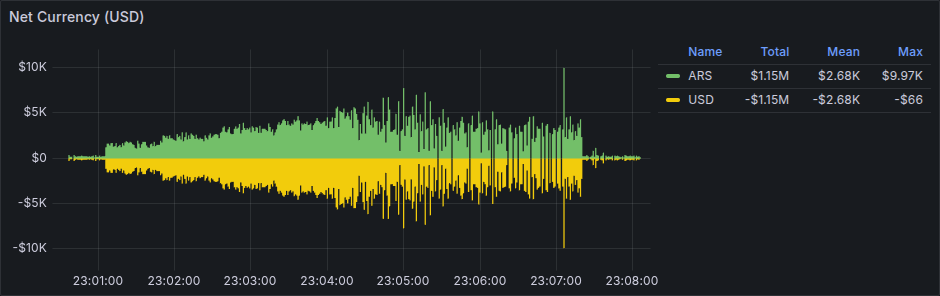
\includegraphics[width=0.8\columnwidth]{figures/propuesta_3/stress/net_currency_captura}
            \caption{ Se adjunta la captura correspondiente a la Figura~\ref{fig:resultados_completos_propuesta_3_stress_net_currency}. }
            \label{fig:resultados_completos_propuesta_3_stress_net_currency_captura}
        \end{figure}

    \clearpage

    \subsection{Resultados completos del escenario de resistencia sobre la propuesta 3}
    \label{sec:resultados_completos_propuesta_3_soak}

        \begin{figure}[H]
            \centering
            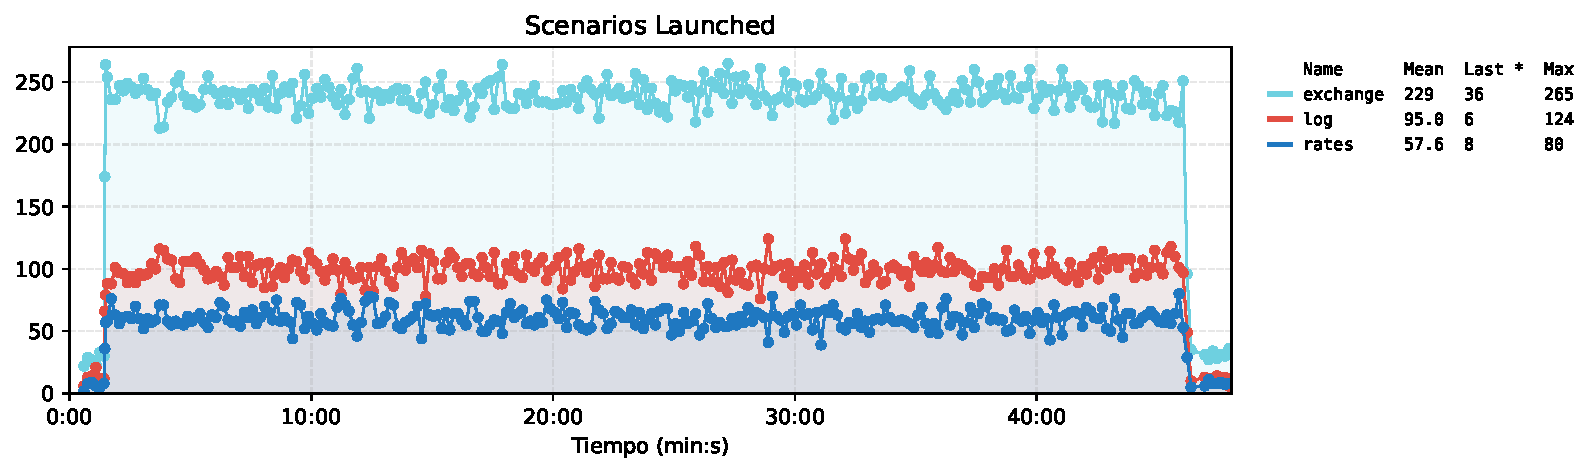
\includegraphics[width=0.8\columnwidth]{figures/propuesta_3/soak/scenarios}
            \caption{ Escenarios de la propuesta 3. }
            \label{fig:resultados_completos_propuesta_3_soak_scenarios}
        \end{figure}

        \begin{figure}[H]
            \centering
            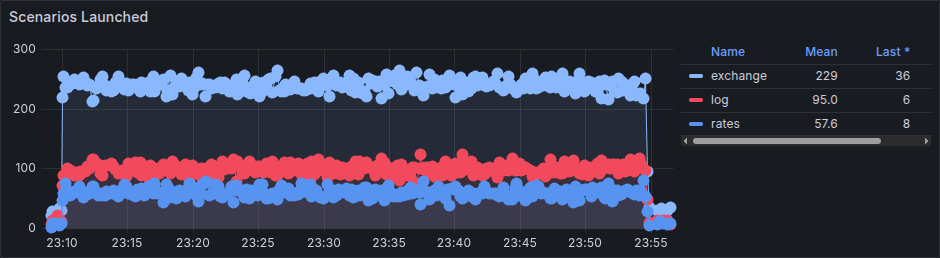
\includegraphics[width=0.8\columnwidth]{figures/propuesta_3/soak/scenarios_captura}
            \caption{ Se adjunta la captura correspondiente a la Figura~\ref{fig:resultados_completos_propuesta_3_soak_scenarios}. }
            \label{fig:resultados_completos_propuesta_3_soak_scenarios_captura}
        \end{figure}

        \begin{figure}[H]
            \centering
            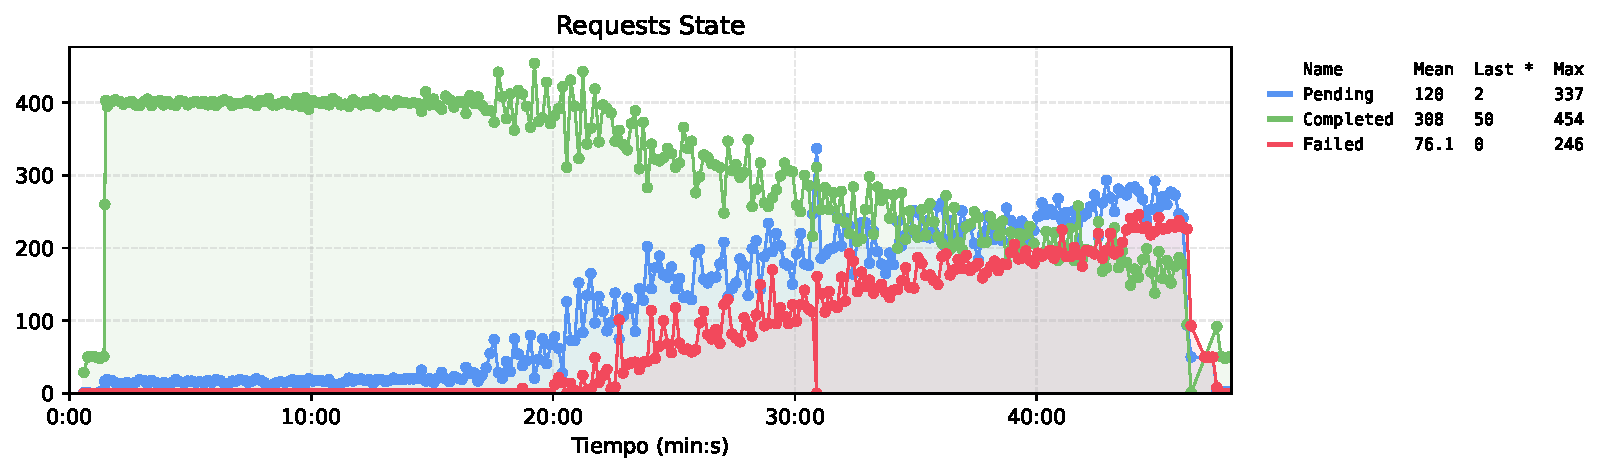
\includegraphics[width=0.8\columnwidth]{figures/propuesta_3/soak/requests_state}
            \caption{ Estado de las requests de la propuesta 3. }
            \label{fig:resultados_completos_propuesta_3_soak_requests_state}
        \end{figure}

        \begin{figure}[H]
            \centering
            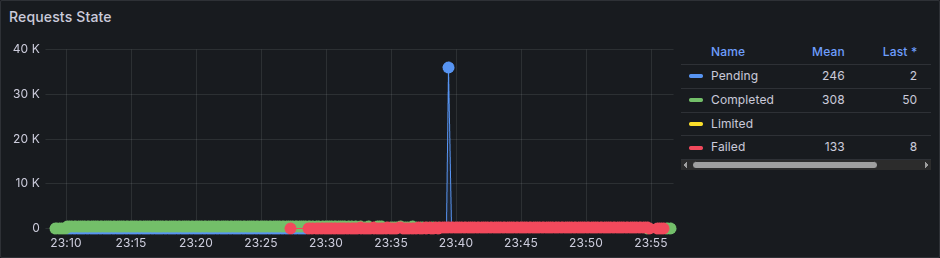
\includegraphics[width=0.8\columnwidth]{figures/propuesta_3/soak/requests_state_captura}
            \caption{ Se adjunta la captura correspondiente a la Figura~\ref{fig:resultados_completos_propuesta_3_soak_requests_state}. }
            \label{fig:resultados_completos_propuesta_3_soak_requests_state_captura}
        \end{figure}

        \begin{figure}[H]
            \centering
            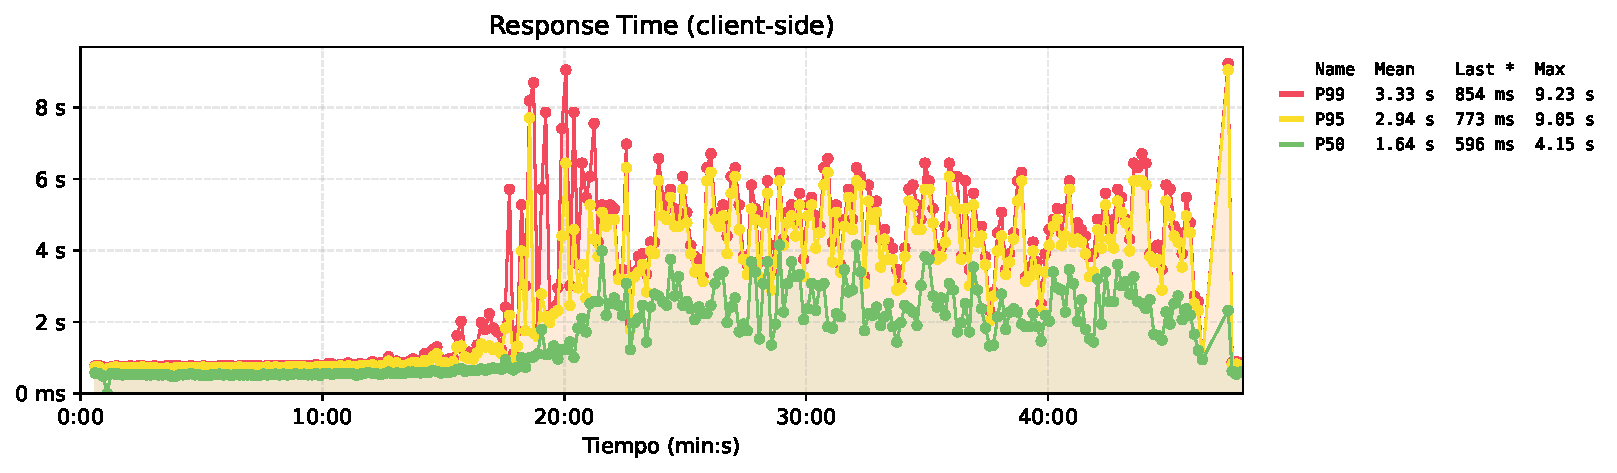
\includegraphics[width=0.8\columnwidth]{figures/propuesta_3/soak/response_time}
            \caption{ Tiempo de respuesta de la propuesta 3. }
            \label{fig:resultados_completos_propuesta_3_soak_response_time}
        \end{figure}

        \begin{figure}[H]
            \centering
            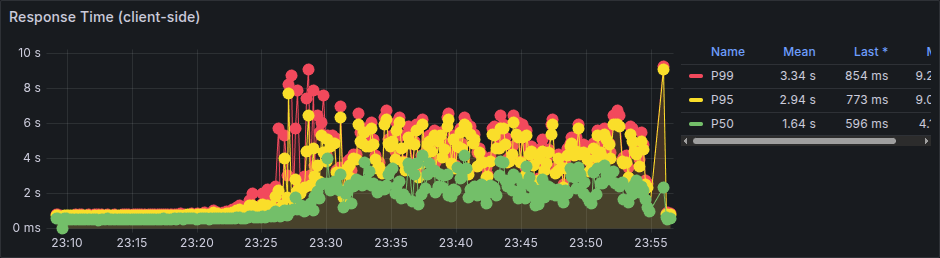
\includegraphics[width=0.8\columnwidth]{figures/propuesta_3/soak/response_time_captura}
            \caption{ Se adjunta la captura correspondiente a la Figura~\ref{fig:resultados_completos_propuesta_3_soak_response_time}. }
            \label{fig:resultados_completos_propuesta_3_soak_response_time_captura}
        \end{figure}

        \begin{figure}[H]
            \centering
            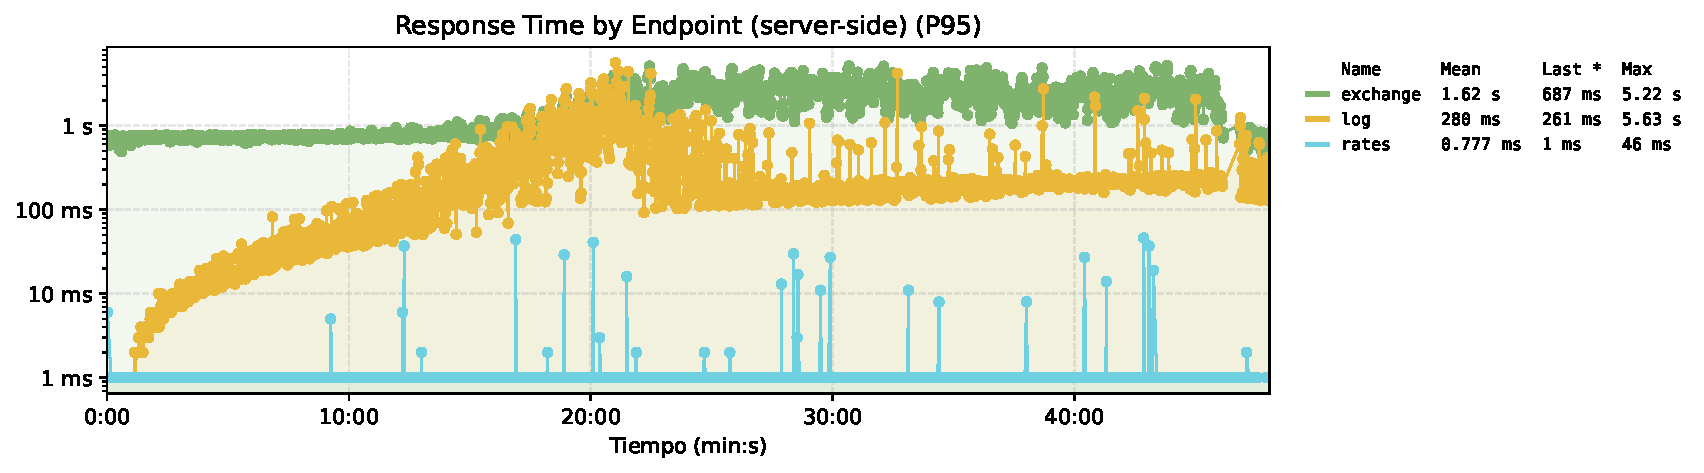
\includegraphics[width=0.8\columnwidth]{figures/propuesta_3/soak/endpoint_response_time}
            \caption{
                Tiempo de respuesta por endpoint de la propuesta 3.
                El eje tiene una escala logarítmica.
            }
            \label{fig:resultados_completos_propuesta_3_soak_endpoint_response_time}
        \end{figure}

        \begin{figure}[H]
            \centering
            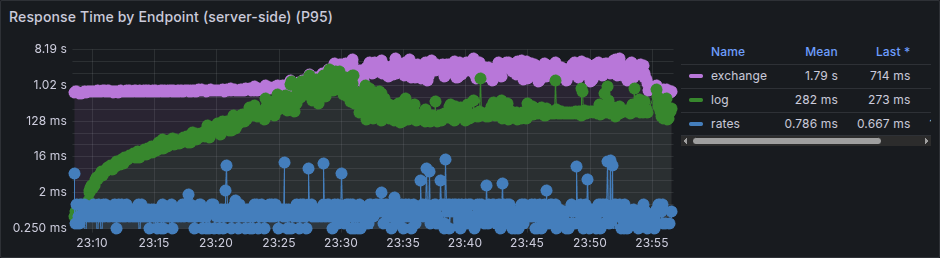
\includegraphics[width=0.8\columnwidth]{figures/propuesta_3/soak/endpoint_response_time_captura}
            \caption{ Se adjunta la captura correspondiente a la Figura~\ref{fig:resultados_completos_propuesta_3_soak_endpoint_response_time}. }
            \label{fig:resultados_completos_propuesta_3_soak_endpoint_response_time_captura}
        \end{figure}

        \begin{figure}[H]
            \centering
            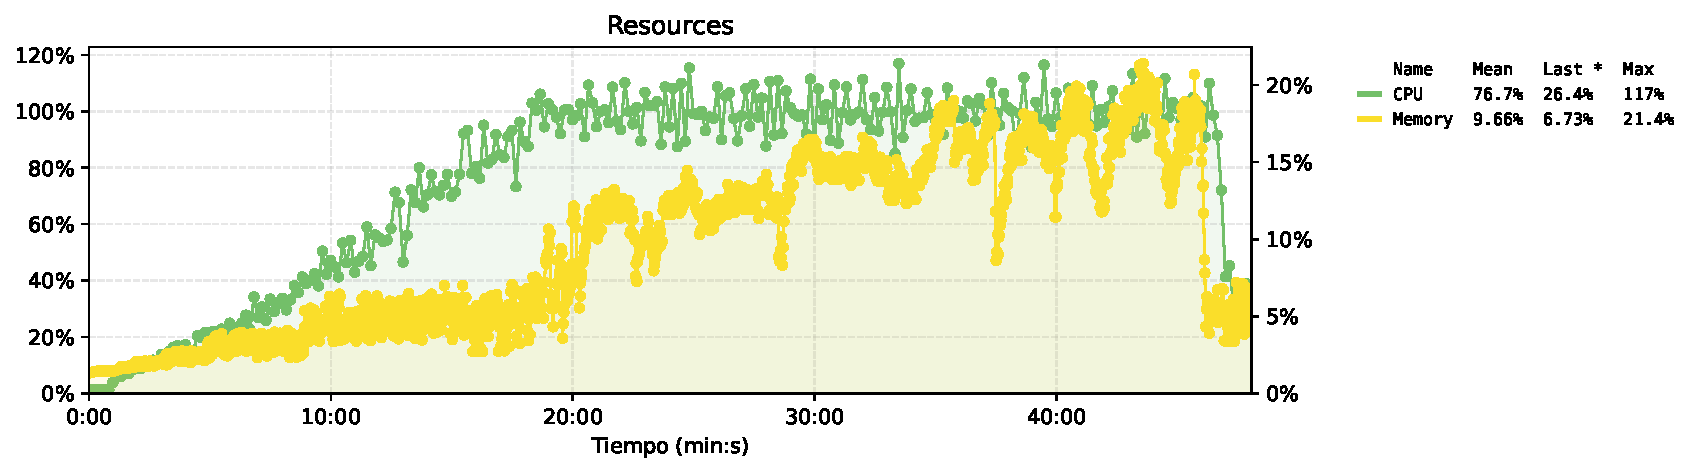
\includegraphics[width=0.8\columnwidth]{figures/propuesta_3/soak/resources}
            \caption{
                Estado de los recursos de la propuesta 3.
                El eje izquierdo muestra el uso de CPU, el eje derecho muestra el uso de memoria.
            }
            \label{fig:resultados_completos_propuesta_3_soak_resources}
        \end{figure}

        \begin{figure}[H]
            \centering
            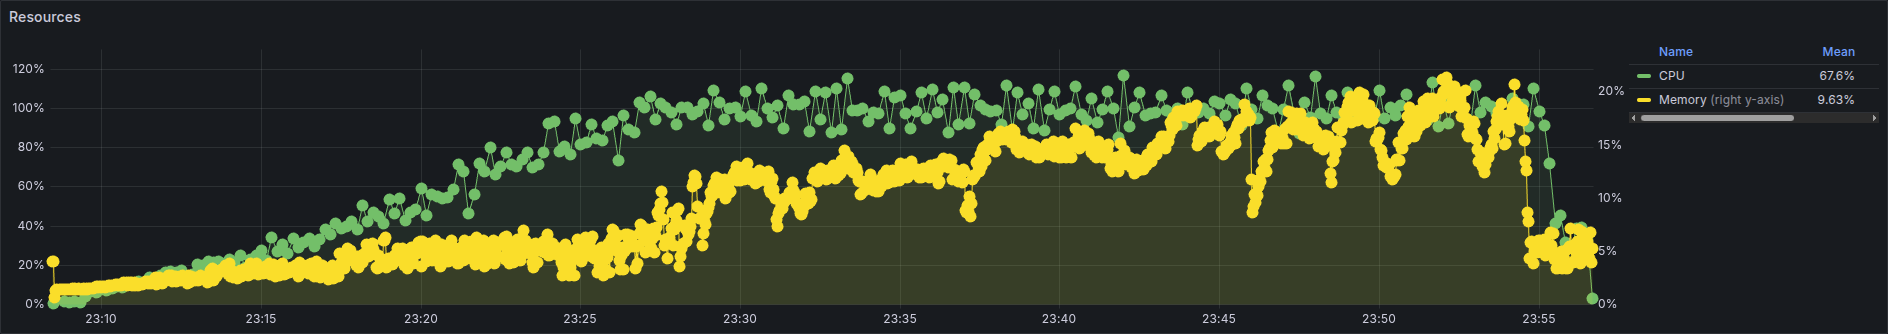
\includegraphics[width=0.8\columnwidth]{figures/propuesta_3/soak/resources_captura}
            \caption{ Se adjunta la captura correspondiente a la Figura~\ref{fig:resultados_completos_propuesta_3_soak_resources}. }
            \label{fig:resultados_completos_propuesta_3_soak_resources_captura}
        \end{figure}

        \begin{figure}[H]
            \centering
            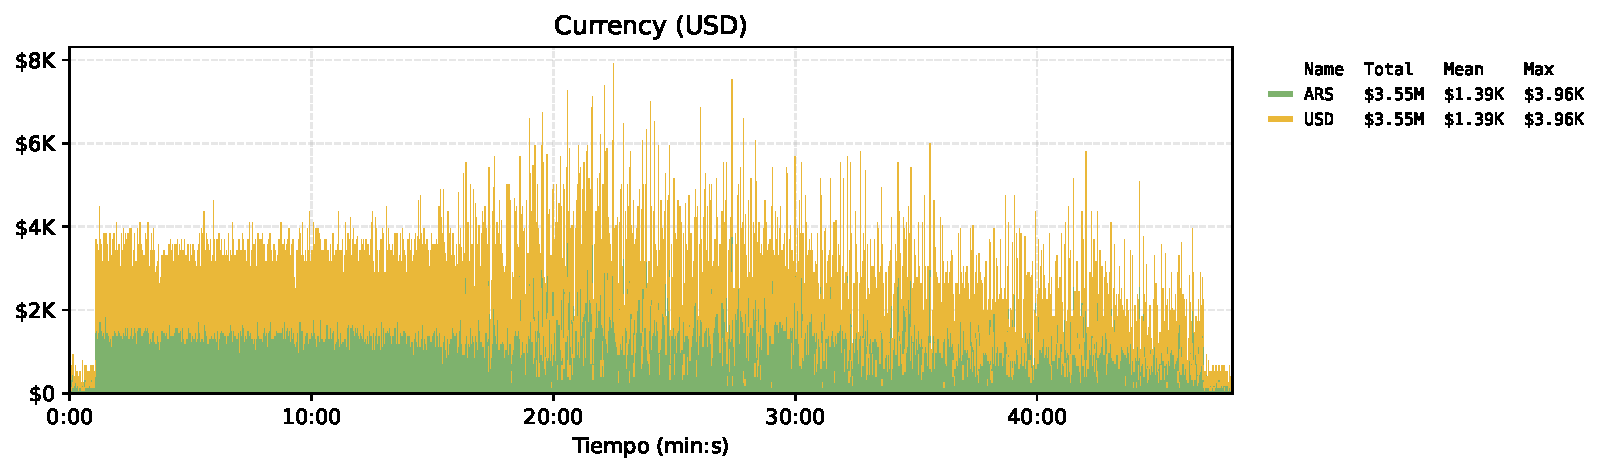
\includegraphics[width=0.8\columnwidth]{figures/propuesta_3/soak/currency}
            \caption{ Volumen operado en cada moneda en la propuesta 3. }
            \label{fig:resultados_completos_propuesta_3_soak_currency}
        \end{figure}

        \begin{figure}[H]
            \centering
            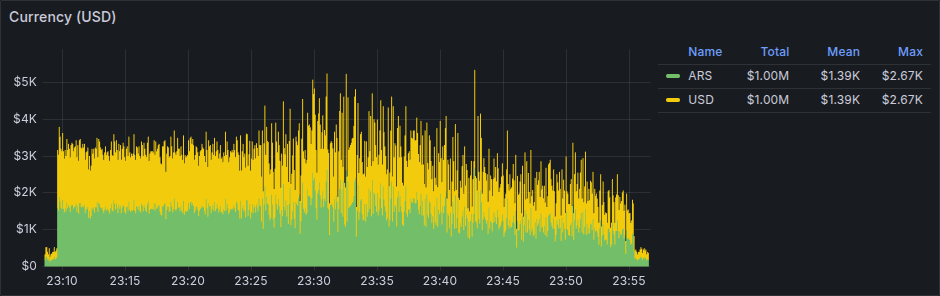
\includegraphics[width=0.8\columnwidth]{figures/propuesta_3/soak/currency_captura}
            \caption{ Se adjunta la captura correspondiente a la Figura~\ref{fig:resultados_completos_propuesta_3_soak_currency}. }
            \label{fig:resultados_completos_propuesta_3_soak_currency_captura}
        \end{figure}

        \begin{figure}[H]
            \centering
            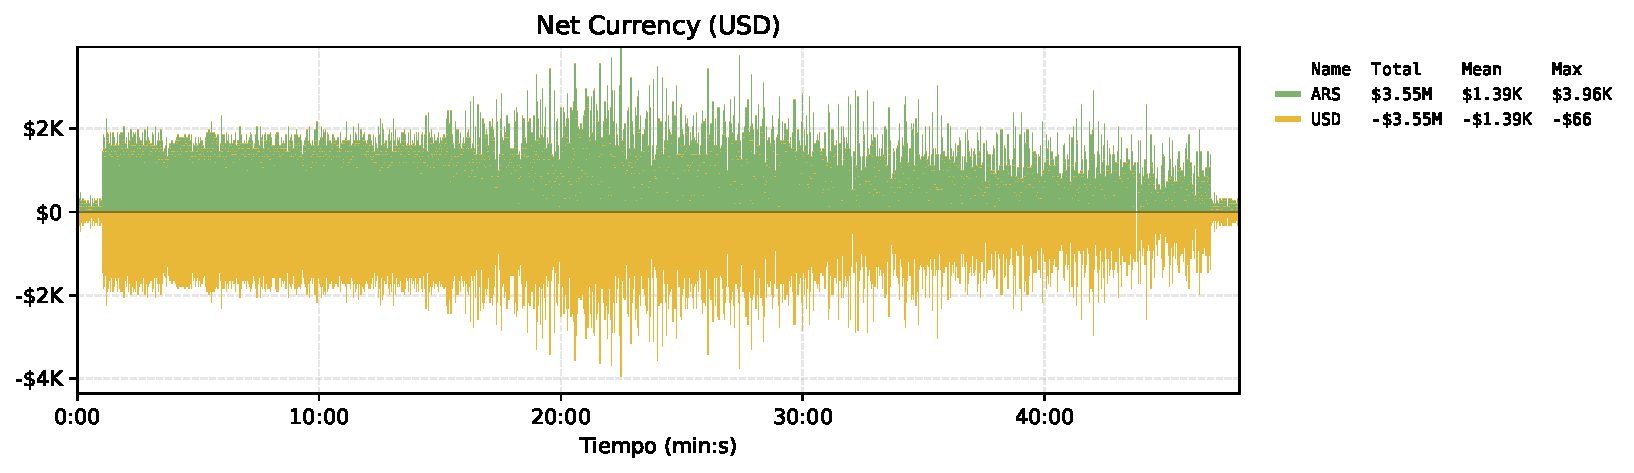
\includegraphics[width=0.8\columnwidth]{figures/propuesta_3/soak/net_currency}
            \caption{ Neto operado en cada moneda en la propuesta 3. }
            \label{fig:resultados_completos_propuesta_3_soak_net_currency}
        \end{figure}

        \begin{figure}[H]
            \centering
            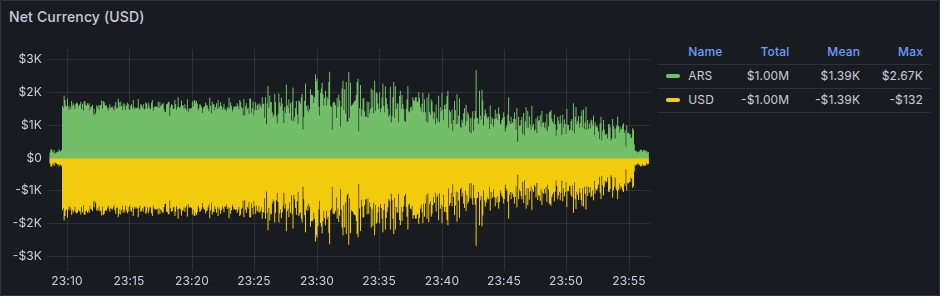
\includegraphics[width=0.8\columnwidth]{figures/propuesta_3/soak/net_currency_captura}
            \caption{ Se adjunta la captura correspondiente a la Figura~\ref{fig:resultados_completos_propuesta_3_soak_net_currency}. }
            \label{fig:resultados_completos_propuesta_3_soak_net_currency_captura}
        \end{figure}

    \clearpage

    \subsection{Resultados completos del escenario de caos sobre la propuesta 3}
    \label{sec:resultados_completos_propuesta_3_chaos}

        \begin{figure}[H]
            \centering
            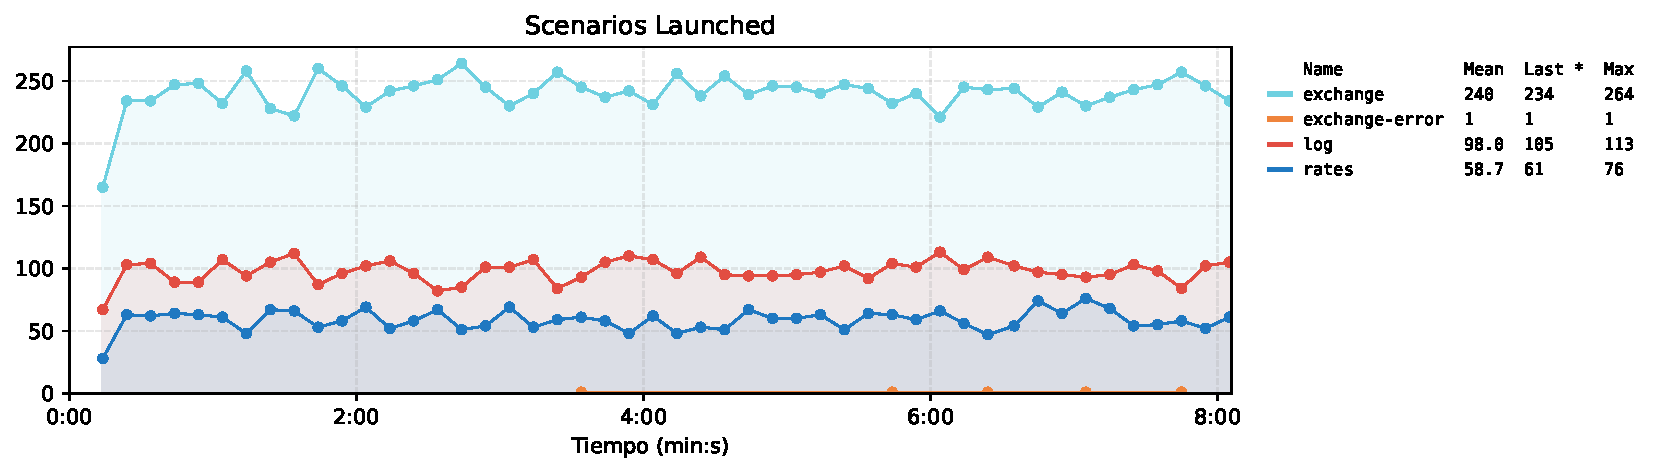
\includegraphics[width=0.8\columnwidth]{figures/propuesta_3/chaos/scenarios}
            \caption{ Escenarios de la propuesta 3. }
            \label{fig:resultados_completos_propuesta_3_chaos_scenarios}
        \end{figure}

        \begin{figure}[H]
            \centering
            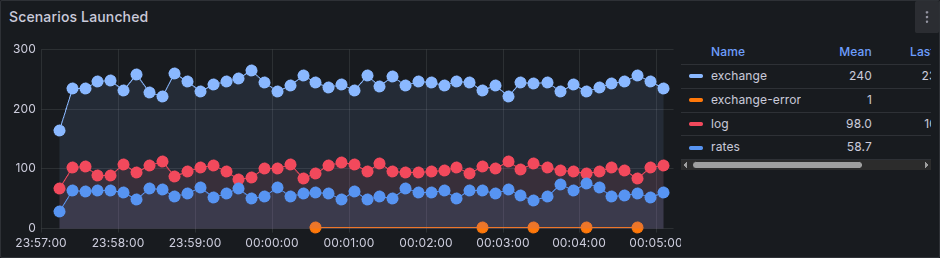
\includegraphics[width=0.8\columnwidth]{figures/propuesta_3/chaos/scenarios_captura}
            \caption{ Se adjunta la captura correspondiente a la Figura~\ref{fig:resultados_completos_propuesta_3_chaos_scenarios}. }
            \label{fig:resultados_completos_propuesta_3_chaos_scenarios_captura}
        \end{figure}

        \begin{figure}[H]
            \centering
            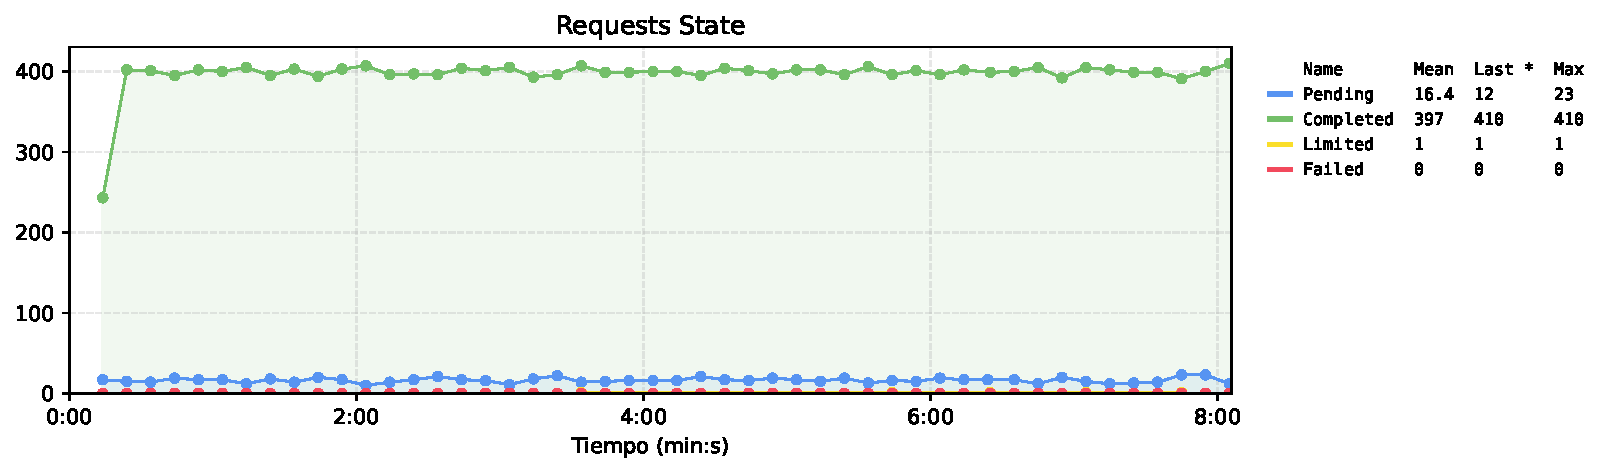
\includegraphics[width=0.8\columnwidth]{figures/propuesta_3/chaos/requests_state}
            \caption{ Estado de las requests de la propuesta 3. }
            \label{fig:resultados_completos_propuesta_3_chaos_requests_state}
        \end{figure}

        \begin{figure}[H]
            \centering
            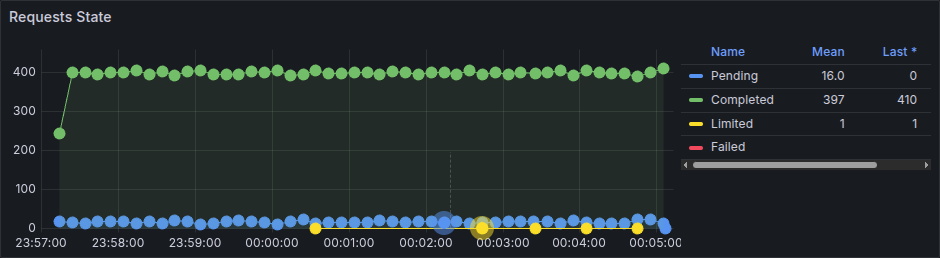
\includegraphics[width=0.8\columnwidth]{figures/propuesta_3/chaos/requests_state_captura}
            \caption{ Se adjunta la captura correspondiente a la Figura~\ref{fig:resultados_completos_propuesta_3_chaos_requests_state}. }
            \label{fig:resultados_completos_propuesta_3_chaos_requests_state_captura}
        \end{figure}

        \begin{figure}[H]
            \centering
            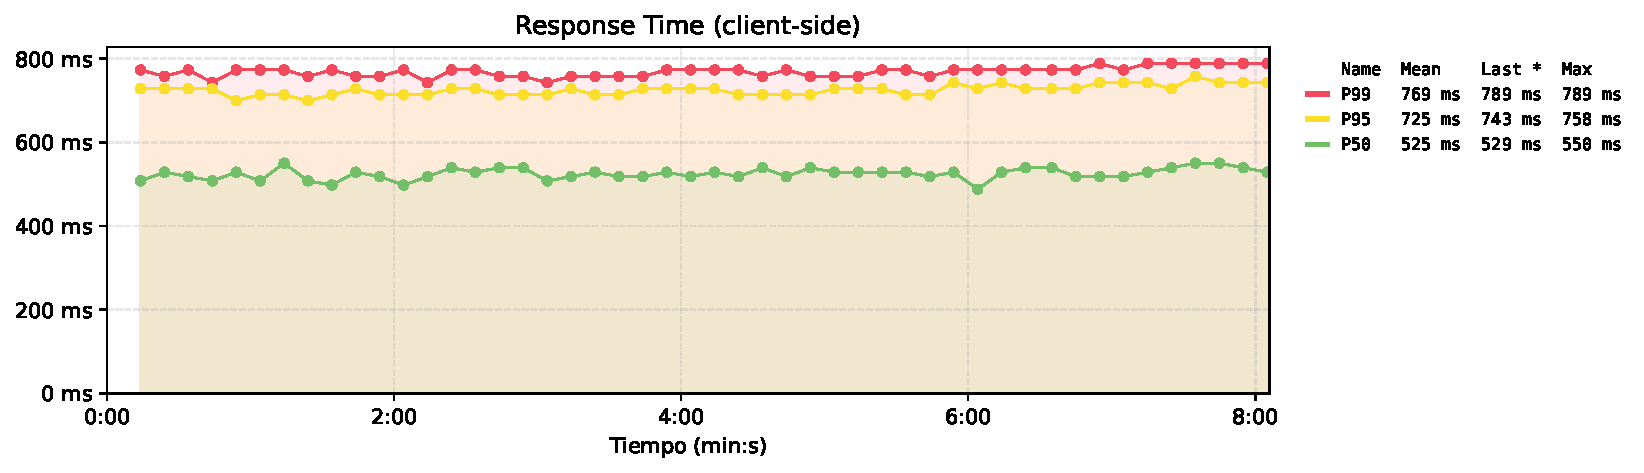
\includegraphics[width=0.8\columnwidth]{figures/propuesta_3/chaos/response_time}
            \caption{ Tiempo de respuesta de la propuesta 3. }
            \label{fig:resultados_completos_propuesta_3_chaos_response_time}
        \end{figure}

        \begin{figure}[H]
            \centering
            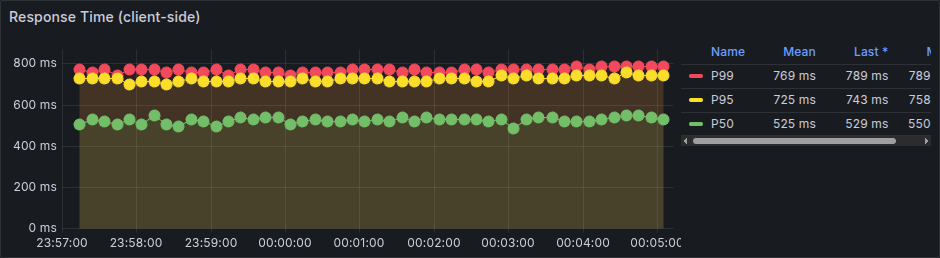
\includegraphics[width=0.8\columnwidth]{figures/propuesta_3/chaos/response_time_captura}
            \caption{ Se adjunta la captura correspondiente a la Figura~\ref{fig:resultados_completos_propuesta_3_chaos_response_time}. }
            \label{fig:resultados_completos_propuesta_3_chaos_response_time_captura}
        \end{figure}

        \begin{figure}[H]
            \centering
            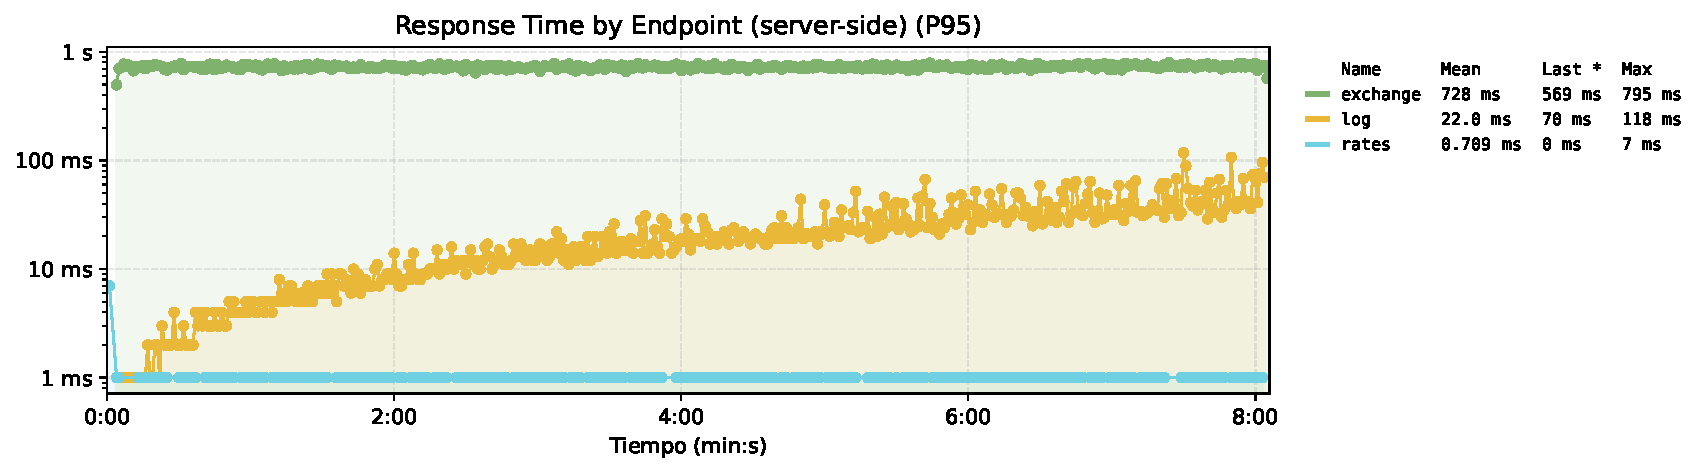
\includegraphics[width=0.8\columnwidth]{figures/propuesta_3/chaos/endpoint_response_time}
            \caption{
                Tiempo de respuesta por endpoint de la propuesta 3.
                El eje tiene una escala logarítmica.
            }
            \label{fig:resultados_completos_propuesta_3_chaos_endpoint_response_time}
        \end{figure}

        \begin{figure}[H]
            \centering
            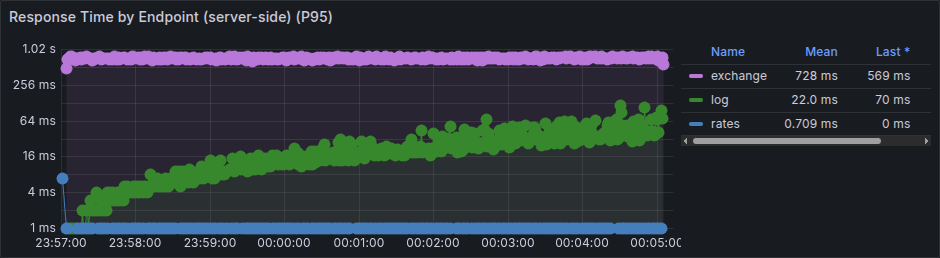
\includegraphics[width=0.8\columnwidth]{figures/propuesta_3/chaos/endpoint_response_time_captura}
            \caption{ Se adjunta la captura correspondiente a la Figura~\ref{fig:resultados_completos_propuesta_3_chaos_endpoint_response_time}. }
            \label{fig:resultados_completos_propuesta_3_chaos_endpoint_response_time_captura}
        \end{figure}

        \begin{figure}[H]
            \centering
            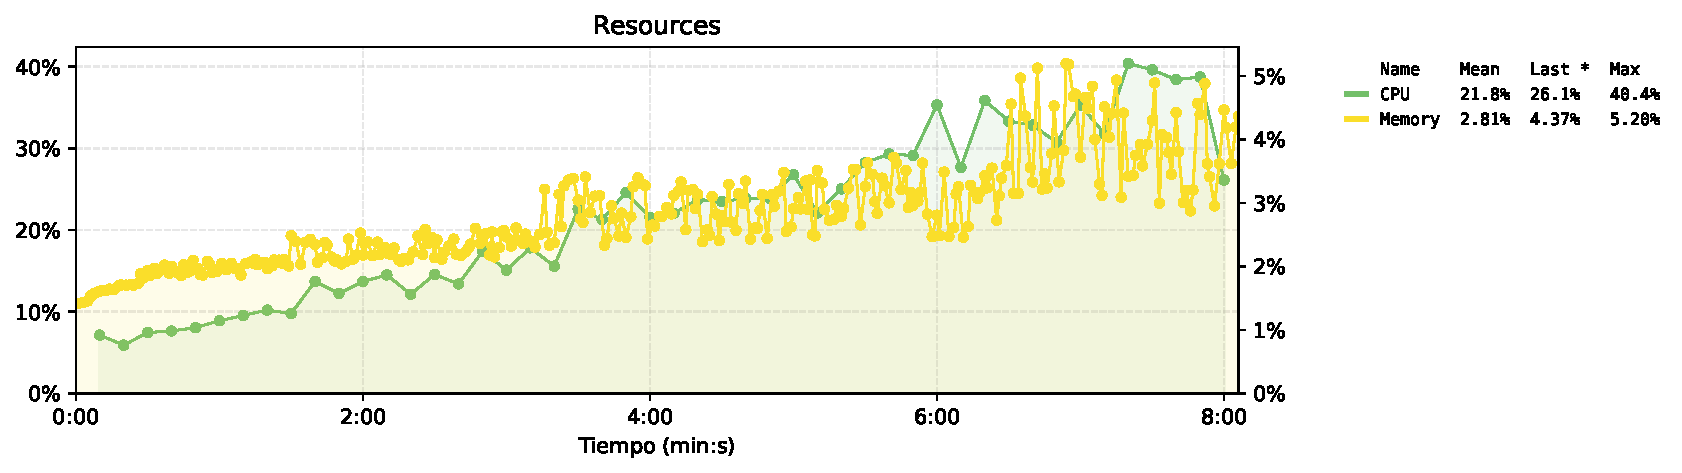
\includegraphics[width=0.8\columnwidth]{figures/propuesta_3/chaos/resources}
            \caption{
                Estado de los recursos de la propuesta 3.
                El eje izquierdo muestra el uso de CPU, el eje derecho muestra el uso de memoria.
            }
            \label{fig:resultados_completos_propuesta_3_chaos_resources}
        \end{figure}

        \begin{figure}[H]
            \centering
            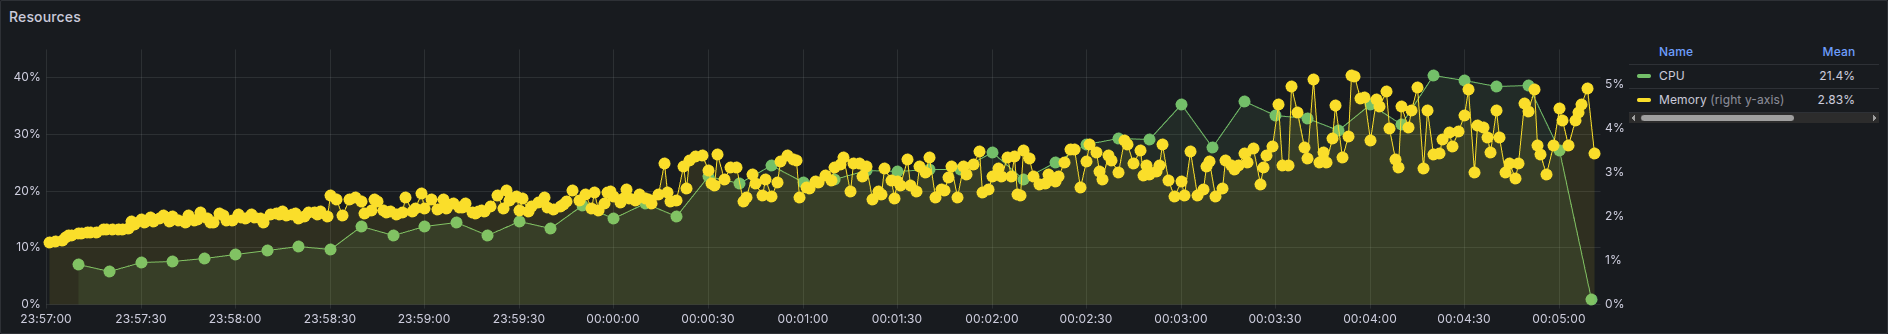
\includegraphics[width=0.8\columnwidth]{figures/propuesta_3/chaos/resources_captura}
            \caption{ Se adjunta la captura correspondiente a la Figura~\ref{fig:resultados_completos_propuesta_3_chaos_resources}. }
            \label{fig:resultados_completos_propuesta_3_chaos_resources_captura}
        \end{figure}

        \begin{figure}[H]
            \centering
            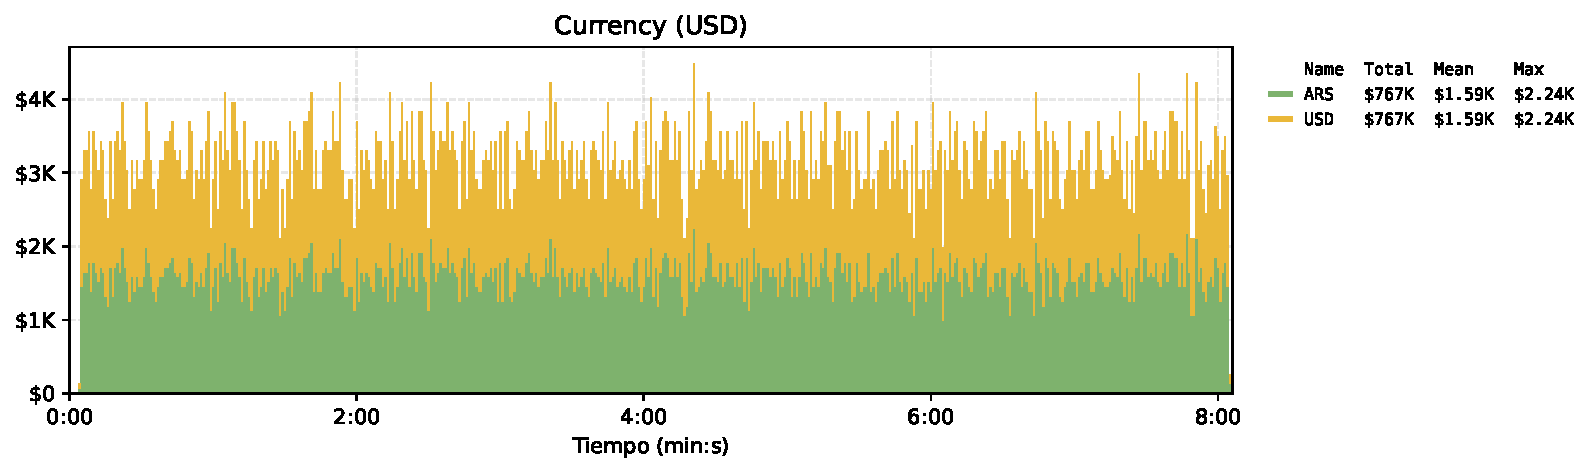
\includegraphics[width=0.8\columnwidth]{figures/propuesta_3/chaos/currency}
            \caption{ Volumen operado en cada moneda en la propuesta 3. }
            \label{fig:resultados_completos_propuesta_3_chaos_currency}
        \end{figure}

        \begin{figure}[H]
            \centering
            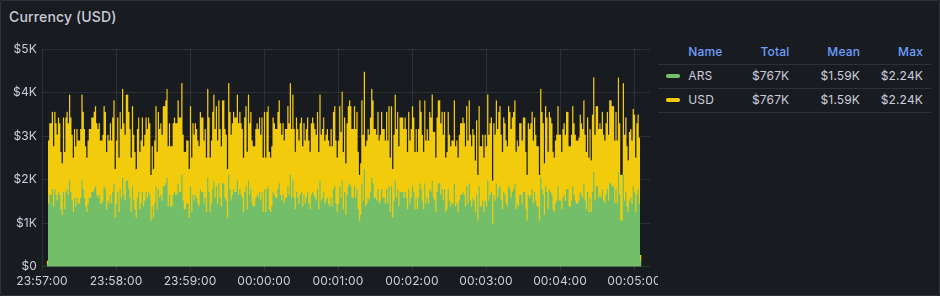
\includegraphics[width=0.8\columnwidth]{figures/propuesta_3/chaos/currency_captura}
            \caption{ Se adjunta la captura correspondiente a la Figura~\ref{fig:resultados_completos_propuesta_3_chaos_currency}. }
            \label{fig:resultados_completos_propuesta_3_chaos_currency_captura}
        \end{figure}

        \begin{figure}[H]
            \centering
            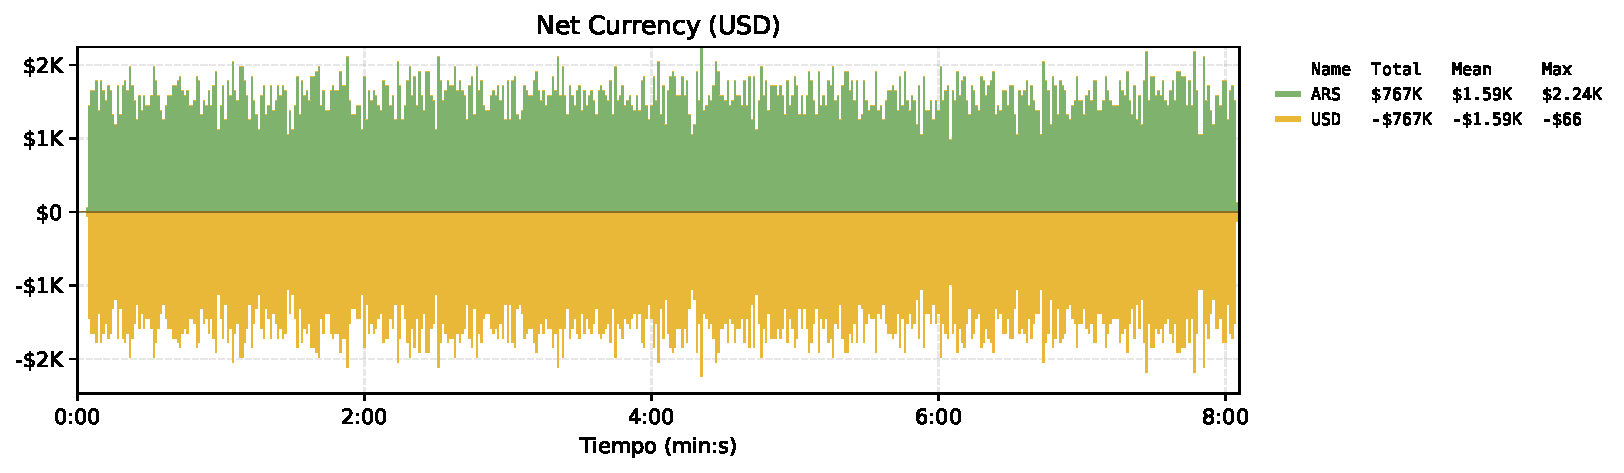
\includegraphics[width=0.8\columnwidth]{figures/propuesta_3/chaos/net_currency}
            \caption{ Neto operado en cada moneda en la propuesta 3. }
            \label{fig:resultados_completos_propuesta_3_chaos_net_currency}
        \end{figure}

        \begin{figure}[H]
            \centering
            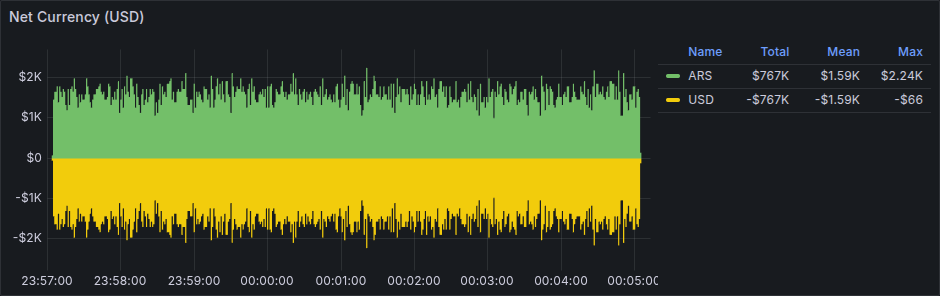
\includegraphics[width=0.8\columnwidth]{figures/propuesta_3/chaos/net_currency_captura}
            \caption{ Se adjunta la captura correspondiente a la Figura~\ref{fig:resultados_completos_propuesta_3_chaos_net_currency}. }
            \label{fig:resultados_completos_propuesta_3_chaos_net_currency_captura}
        \end{figure}

    \clearpage

    \subsection{Resultados completos del escenario de concurrencia sobre la propuesta 3}
    \label{sec:resultados_completos_propuesta_3_race}

        \begin{figure}[H]
            \centering
            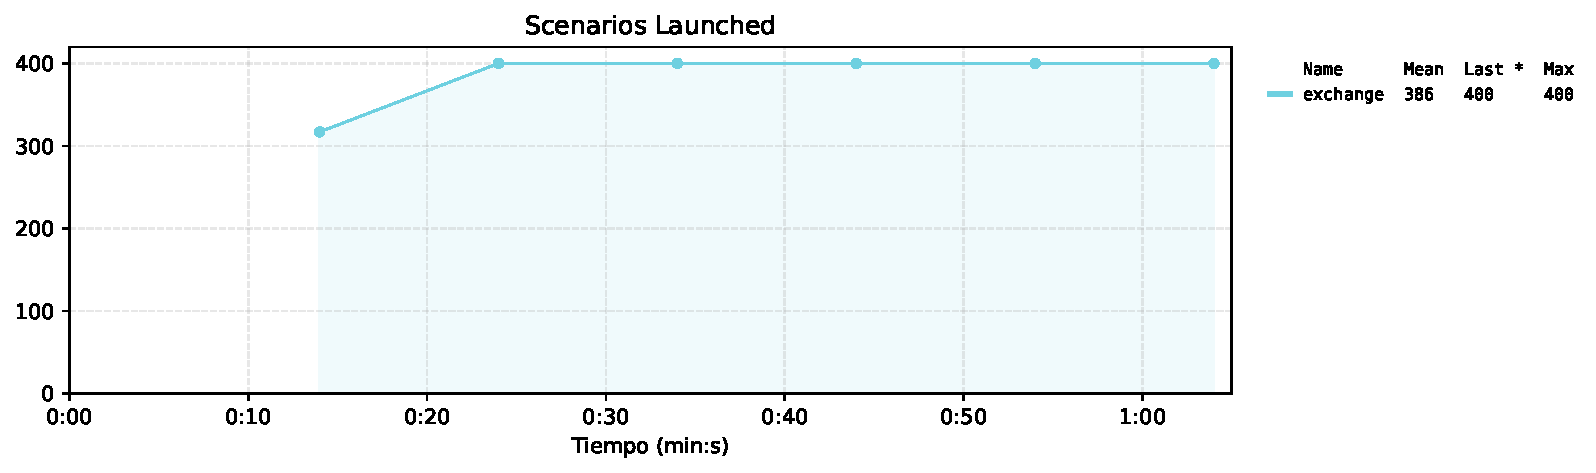
\includegraphics[width=0.8\columnwidth]{figures/propuesta_3/race/scenarios}
            \caption{ Escenarios de la propuesta 3. }
            \label{fig:resultados_completos_propuesta_3_race_scenarios}
        \end{figure}

        \begin{figure}[H]
            \centering
            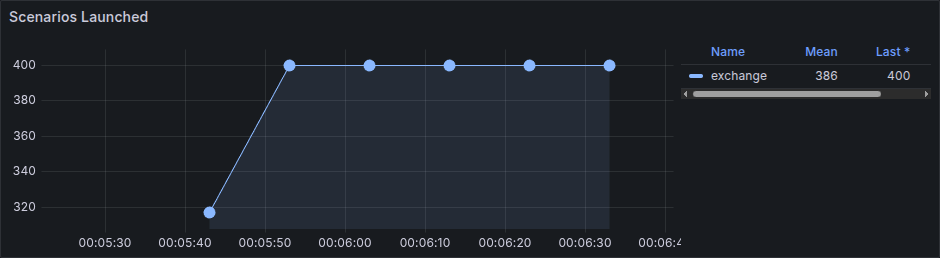
\includegraphics[width=0.8\columnwidth]{figures/propuesta_3/race/scenarios_captura}
            \caption{ Se adjunta la captura correspondiente a la Figura~\ref{fig:resultados_completos_propuesta_3_race_scenarios}. }
            \label{fig:resultados_completos_propuesta_3_race_scenarios_captura}
        \end{figure}

        \begin{figure}[H]
            \centering
            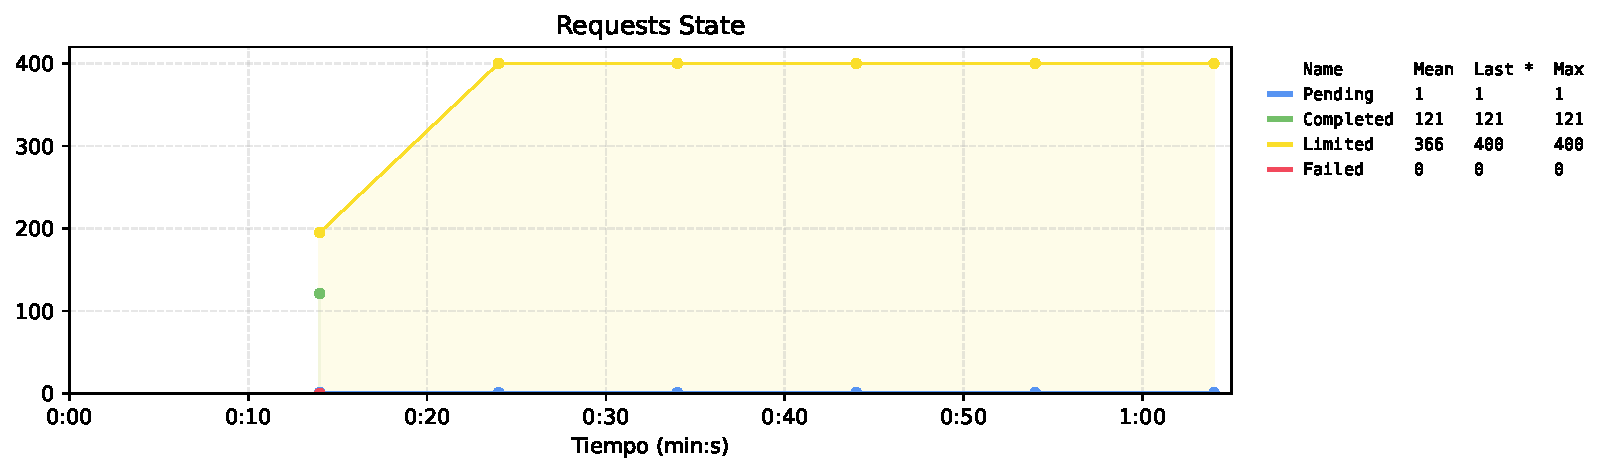
\includegraphics[width=0.8\columnwidth]{figures/propuesta_3/race/requests_state}
            \caption{ Estado de las requests de la propuesta 3. }
            \label{fig:resultados_completos_propuesta_3_race_requests_state}
        \end{figure}

        \begin{figure}[H]
            \centering
            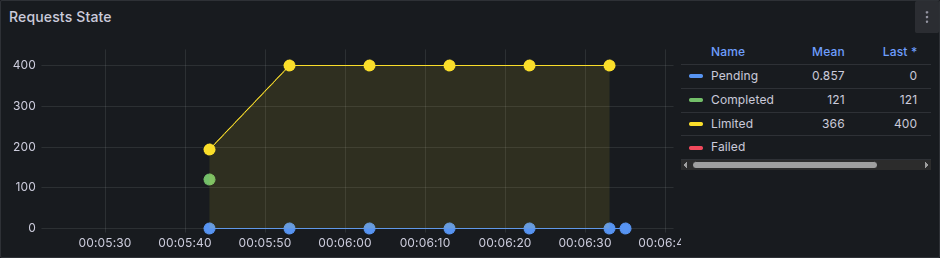
\includegraphics[width=0.8\columnwidth]{figures/propuesta_3/race/requests_state_captura}
            \caption{ Se adjunta la captura correspondiente a la Figura~\ref{fig:resultados_completos_propuesta_3_race_requests_state}. }
            \label{fig:resultados_completos_propuesta_3_race_requests_state_captura}
        \end{figure}

        \begin{figure}[H]
            \centering
            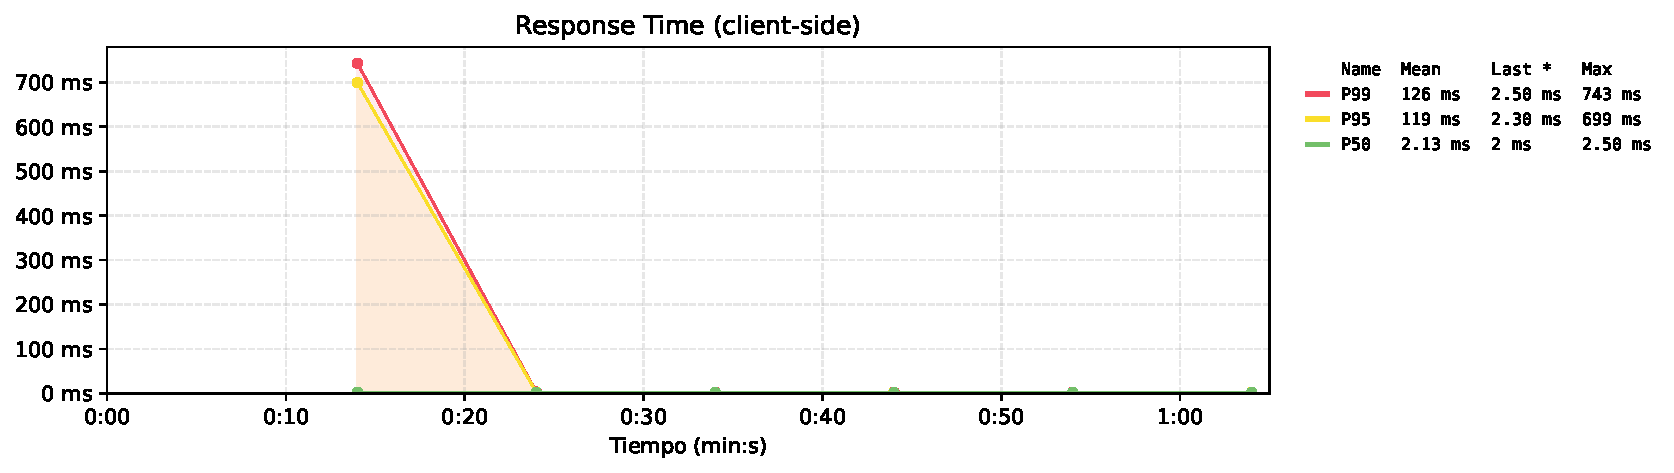
\includegraphics[width=0.8\columnwidth]{figures/propuesta_3/race/response_time}
            \caption{ Tiempo de respuesta de la propuesta 3. }
            \label{fig:resultados_completos_propuesta_3_race_response_time}
        \end{figure}

        \begin{figure}[H]
            \centering
            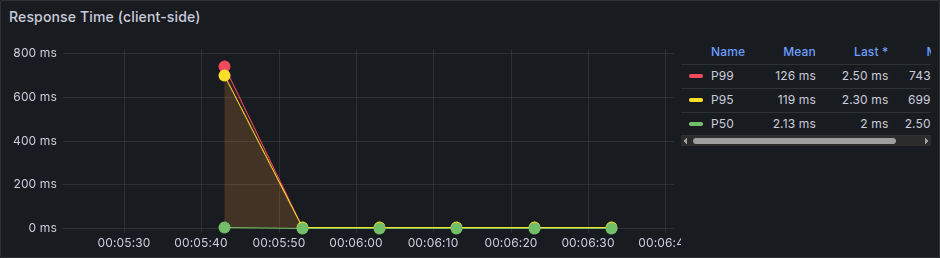
\includegraphics[width=0.8\columnwidth]{figures/propuesta_3/race/response_time_captura}
            \caption{ Se adjunta la captura correspondiente a la Figura~\ref{fig:resultados_completos_propuesta_3_race_response_time}. }
            \label{fig:resultados_completos_propuesta_3_race_response_time_captura}
        \end{figure}

        \begin{figure}[H]
            \centering
            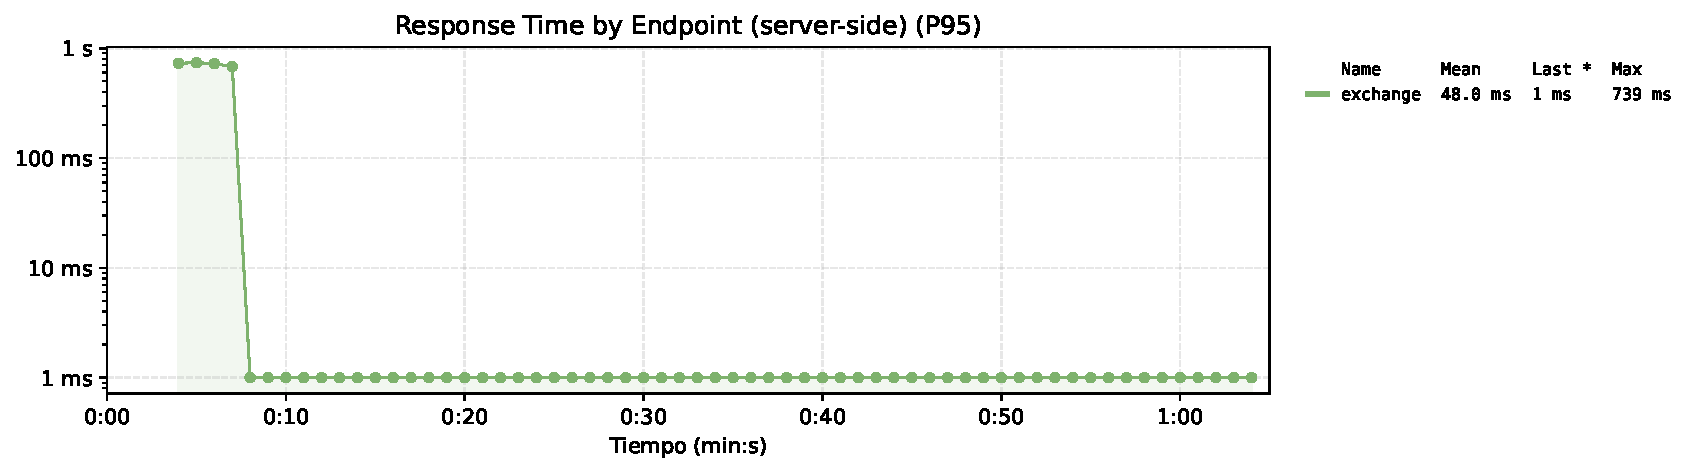
\includegraphics[width=0.8\columnwidth]{figures/propuesta_3/race/endpoint_response_time}
            \caption{
                Tiempo de respuesta por endpoint de la propuesta 3.
                El eje tiene una escala logarítmica.
            }
            \label{fig:resultados_completos_propuesta_3_race_endpoint_response_time}
        \end{figure}

        \begin{figure}[H]
            \centering
            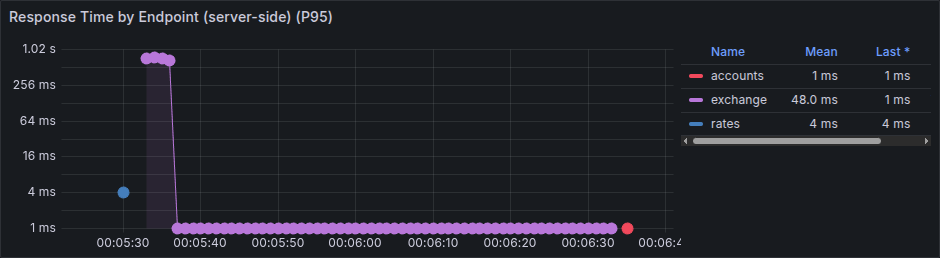
\includegraphics[width=0.8\columnwidth]{figures/propuesta_3/race/endpoint_response_time_captura}
            \caption{ Se adjunta la captura correspondiente a la Figura~\ref{fig:resultados_completos_propuesta_3_race_endpoint_response_time}. }
            \label{fig:resultados_completos_propuesta_3_race_endpoint_response_time_captura}
        \end{figure}

        \begin{figure}[H]
            \centering
            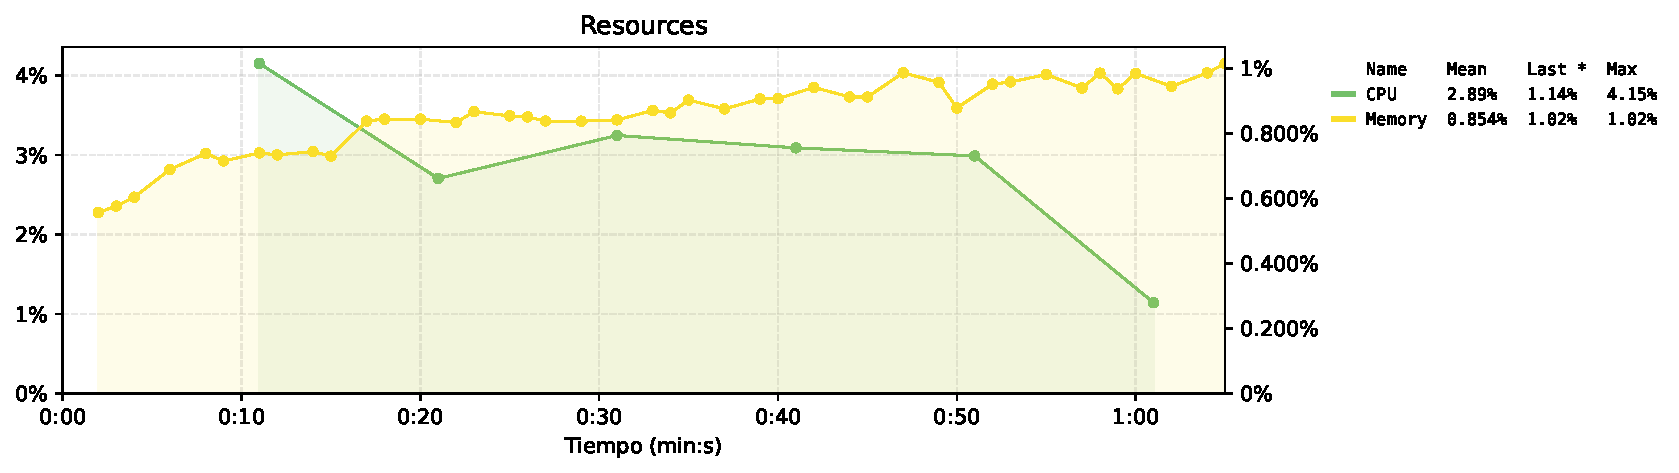
\includegraphics[width=0.8\columnwidth]{figures/propuesta_3/race/resources}
            \caption{
                Estado de los recursos de la propuesta 3.
                El eje izquierdo muestra el uso de CPU, el eje derecho muestra el uso de memoria.
            }
            \label{fig:resultados_completos_propuesta_3_race_resources}
        \end{figure}

        \begin{figure}[H]
            \centering
            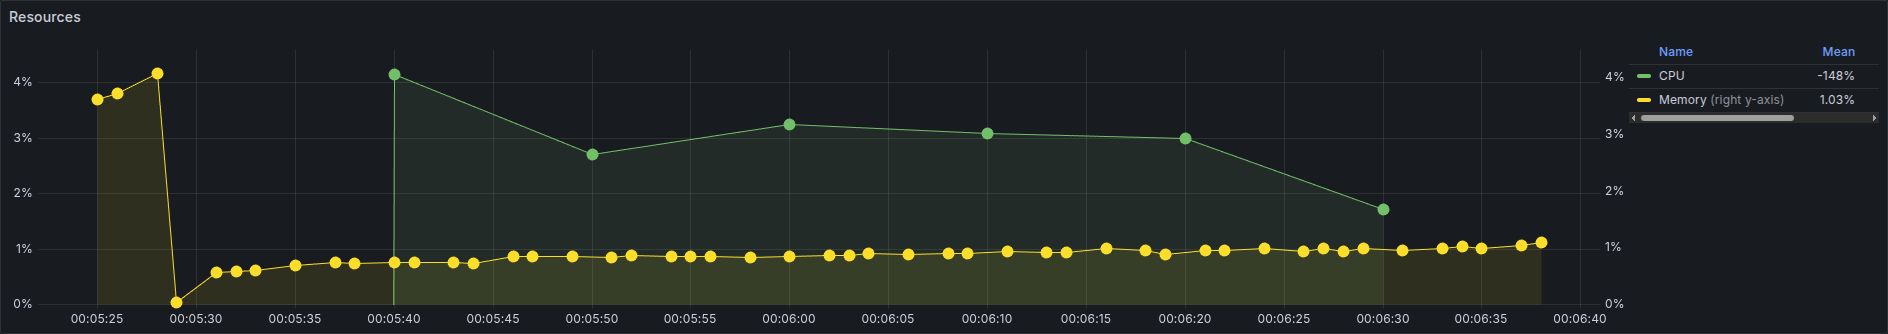
\includegraphics[width=0.8\columnwidth]{figures/propuesta_3/race/resources_captura}
            \caption{ Se adjunta la captura correspondiente a la Figura~\ref{fig:resultados_completos_propuesta_3_race_resources}. }
            \label{fig:resultados_completos_propuesta_3_race_resources_captura}
        \end{figure}

        \begin{figure}[H]
            \centering
            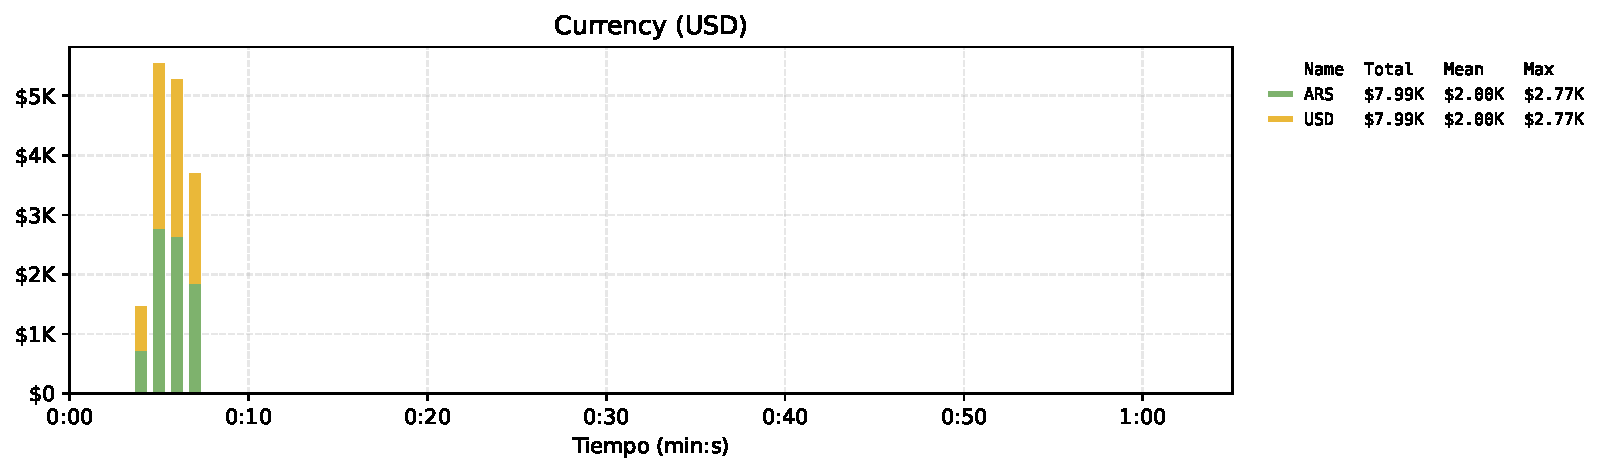
\includegraphics[width=0.8\columnwidth]{figures/propuesta_3/race/currency}
            \caption{ Volumen operado en cada moneda en la propuesta 3. }
            \label{fig:resultados_completos_propuesta_3_race_currency}
        \end{figure}

        \begin{figure}[H]
            \centering
            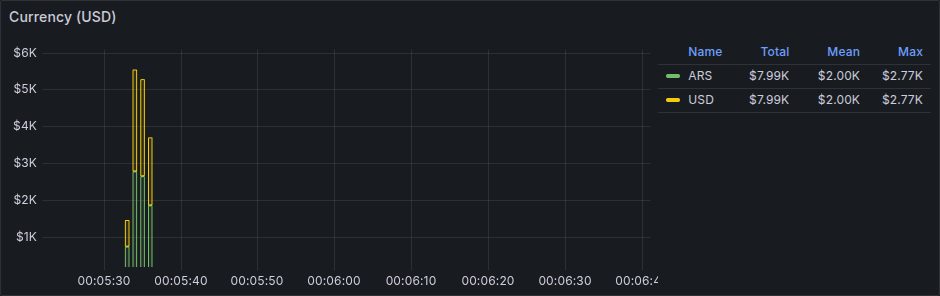
\includegraphics[width=0.8\columnwidth]{figures/propuesta_3/race/currency_captura}
            \caption{ Se adjunta la captura correspondiente a la Figura~\ref{fig:resultados_completos_propuesta_3_race_currency}. }
            \label{fig:resultados_completos_propuesta_3_race_currency_captura}
        \end{figure}

        \begin{figure}[H]
            \centering
            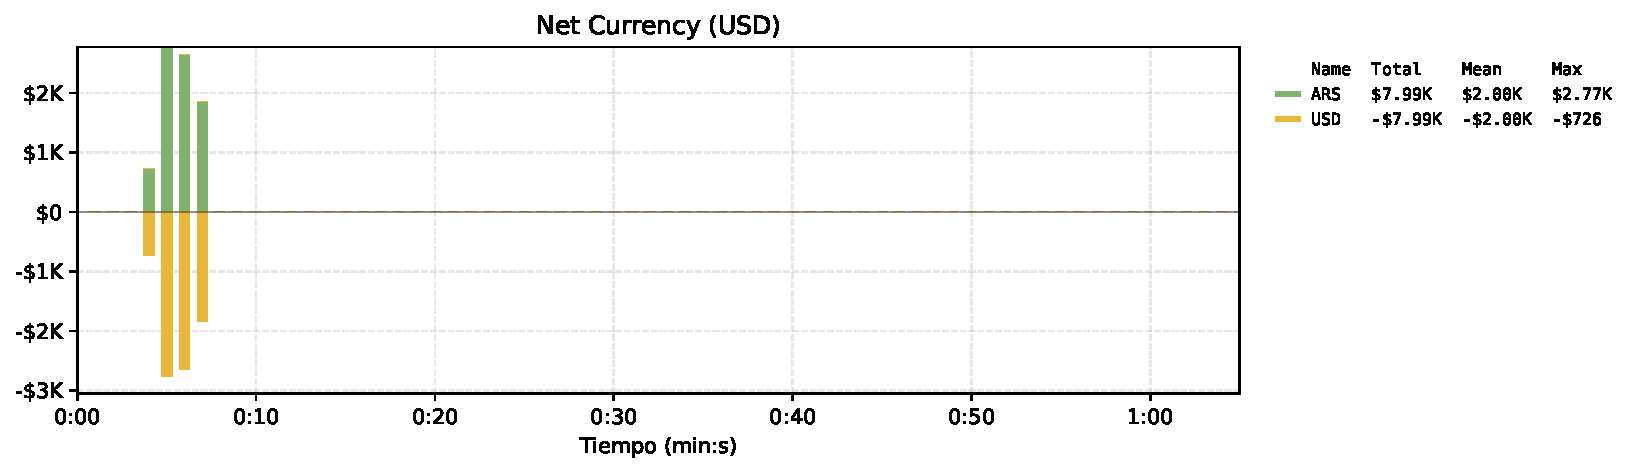
\includegraphics[width=0.8\columnwidth]{figures/propuesta_3/race/net_currency}
            \caption{ Neto operado en cada moneda en la propuesta 3. }
            \label{fig:resultados_completos_propuesta_3_race_net_currency}
        \end{figure}

        \begin{figure}[H]
            \centering
            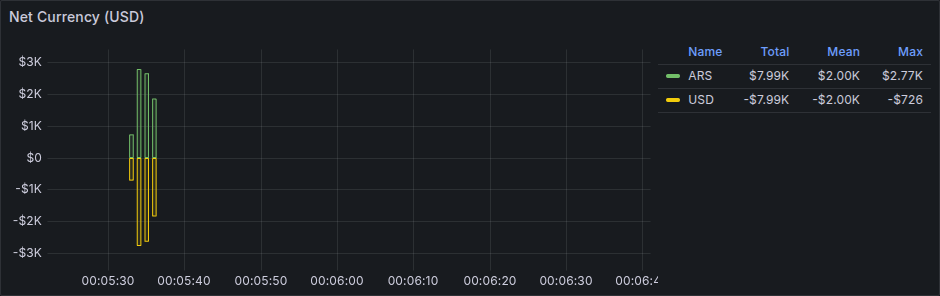
\includegraphics[width=0.8\columnwidth]{figures/propuesta_3/race/net_currency_captura}
            \caption{ Se adjunta la captura correspondiente a la Figura~\ref{fig:resultados_completos_propuesta_3_race_net_currency}. }
            \label{fig:resultados_completos_propuesta_3_race_net_currency_captura}
        \end{figure}
